\documentclass[a4paper]{amsbook}

% AMSMath-packages
\usepackage{amsthm}
\usepackage{amssymb}
\usepackage{amsrefs}
\usepackage{textcmds}

% ISO Latin 1 input encoding
\usepackage{t1enc}
\usepackage[latin1]{inputenc}
\usepackage[T1]{fontenc}

% Vector fonts for PDF
\usepackage{ae}

% Graphics for figures
\usepackage{graphicx}

% Correct font scaling in formulas
\usepackage{exscale}

% Use "makeindex" package
%\usepackage{makeidx}

% My own math commands
\usepackage{jkmath}

\usepackage{subfigure}

\theoremstyle{plain}
\newtheorem{theorem}{Theorem}[chapter]
\newtheorem{corollary}[theorem]{Corollary}
\newtheorem{lemma}[theorem]{Lemma}
\newtheorem{proposition}[theorem]{Proposition}
\theoremstyle{definition}
\newtheorem{definition}[theorem]{Definition}
\newtheorem{example}[theorem]{Example}
\theoremstyle{remark}
\newtheorem{remark}[theorem]{Remark}

\numberwithin{figure}{chapter} 
\numberwithin{table}{chapter} 
\numberwithin{equation}{chapter} 

\makeindex

\begin{document}

\frontmatter

\title{Fast Spherical Fourier Transform}
\author{Jens Keiner}
\email{keiner@math.uni-luebeck.de}
\address{M�hlenstra�e 22-24 \\ 23552 L�beck \\ Germany}
\subjclass{12J32A32}

\maketitle

\tableofcontents

\mainmatter

%\begin{savequote}[8cm]
%  ``Confession: I played golf. Confession: I hired a cleaning lady. Confession: I am owner of the Turbo nose-hair trimmer with optional ear-hair accessory.''
%  \qauthor{Dan Zevin}
%\end{savequote}
%\makeatletter

\chapter*{Introduction}
\label{Introduction}

The \emph{fast Fourier transform (FFT)} has become one of the most important 
and widely used algorithms today. In 1965, Cooley and Tukey (\cite{cotu}) published
and publicized the first description of a fast algorithm for computing certain
trigonometric sums, generally referred to as the \emph{discrete} or 
\emph{finite Fourier transform}. In fact, developments since then, now
let us speak of a whole class of algorithms. The original Culey-Tukey FFT
used a recursive scheme to split one large transform successively into
smaller transforms achieving an asymptotical complexity of 
$\bigo{N \log N}$ \emph{floating point operations (flops)} instead of
$\bigo{N^2}$ for a direct computation, where $N$ is the transform length. 
Efficient and highly optimized implementations also for the
multidimensional case are available (\cite{fftw}).
Surprisingly, the idea of Cooley and Tukey was already described by Gauss around
1805 (\cite{hejobu}) interpolating the trajectories of the asteroids Pallas 
and Juno. But his work was not widely recognized and only published posthumously.
The wide areas of applications nowadays using FFT-techniques, including, for example, 
time-frequency analysis, signal-processing and the numerical solution of 
partial differential equations, underline the great importance and impact of fast
DFT algorithms.
Recently, algorithms have been developed for a more general type of discrete 
transform, namely the \emph{nonuniform discrete Fourier transform (NDFT)}. 
While the DFT is a bijective and easily invertible linear mapping of $N$ 
ingoing coefficients to $N$ outgoing coefficients, corresponding to
uniformly distributed nodes on an interval, the NDFT generalizes
discrete Fourier sums for arbitrary node distributions, hence the name
'nonuniform'. Fast algorithms have been described in several papers 
(\cite{bey95},\cite{duro93},\cite{fesu02},\cite{four},\cite{Ja},\cite{Pe},\cite{scsc},\cite{ware98}) and a C subroutine library is available 
(\cite{kupo02C}).
A different line of generalization leaves the 'classical' setting of 
Fourier series on a multidimensional torus and describes analogously
Fourier series on different geometries like the surface of a
multidimensional sphere. Particularly, the unit sphere $\twosphere$ 
embedded into $\R^3$ has practical relevance in quite a wide range of 
applications, in many cases due to its correspondence to the surface 
of the earth. Fields of interest are numerical analysis in
geo-sciences, for example in the computation of climate models for
weather forecasts, or regarding the gravitational potential of the 
earth. Moreover, data distributed on the surface of a sphere arise
in many other applications in a natural way. Examples are
molecular dynamics for protein docking problems and 
gamma-cameras for applications in computed tomography.
Unfortunately, the spherical setting differs from the 'classical' 
one in that the numerical treatment of many computational problems
is quite more challenging. Also there exists a rich theory for 
analysis on the sphere, fast algorithms allowing for efficient and
reliable discrete transforms in terms of the so-called 
\emph{spherical harmonics}, the spherical counterpart of the 
Fourier basis $\set{e^{\im k x}}_{k \in \Z}$ on the interval,
haven't been developed until a first paper by Driscoll and Healy. 
During the past years, major progress has been made and several 
different techniques have been developed. The common idea is to
transform the spherical discrete Fourier transformation into a
'classical' two-dimensional discrete Fourier transform. The
different proposed algorithms mainly differ in the ansatz chosen
to compute the transformation efficiently. A careful analysis
of numerical instabilities involved has proven to be of major 
importance.

The aim of this text is to describe particular algorithms for fast discrete
spherical Fourier transforms. Chapter \ref{Basics} gives a brief 
introduction to Fourier analysis on the sphere $\twosphere$ and 
provides fundamental facts and results.
In Chapter \ref{DSFT}, algorithms for the computation of discrete
spherical Fourier transforms are derived. We describe the
so-called 'direct' algorithms and the 'fast' algorithms based on
the \emph{fast Legendre function transform (FLFT)}. We also mention
how spherical Fourier coefficients might be computed by certain 
quadrature formulae. Chapter \ref{Applications} finally presents 
two applications of the proposed algorithms along with numerical
test computations.

\chapter{Basics}
\label{Basics}

\section{Notational Conventions}
\label{Basics:Notation}

Every point $\V{\xi} \in \R^3 \setminus \set{\V{0}}$ given in Cartesian coordinates by the vector 
$\paren{x_1,x_2,x_3}^{\transp}$ can be uniquely described in spherical coordinates by a vector
$\paren{r,\vtheta,\vphi}^{\transp}$ with $r \in \Rp$, $\vtheta \in \interv{[}{0}{\pi}{]}$ and 
$\vphi \in \interv{[}{0}{2\pi}{)}$.
It holds 
\begin{eqnarray*}
  \paren{x_1,x_2,x_3}^{\transp} & = & \paren{r \sin \vtheta \cos \vphi, r \sin \vtheta \sin \vphi, r \cos \vtheta}^{\transp}\\
  r & = & \sqrt{x_1^2+x_2^2+x_3^2} = \norm{\V{\xi}}_2.
\end{eqnarray*} 
We denote by $\twosphere$ the $2$-nd unit sphere embedded into $\R^3$, i.e. 
$$\twosphere := \pset{\V{\xi} \in \R^{3}}{|}{\norm{\V{\xi}}_2=1}$$ 
and identify $\V{\xi} \in \twosphere$ with the vector $\paren{\vtheta,\vphi}^{\transp}$. The 
spherical coordinate system is illustrated in Figure \ref{sphere}.

Now let $\V{\xi} = \paren{\vtheta,\vphi}^{\transp}$, $\V{\eta} = \paren{\vtheta',\vphi'}^{\transp} \in
\twosphere$ and $\alpha$ be the angle spanned by the origin, $\V{\xi}$ and $\V{\eta}$.
Then the standard scalar product
$\scalarproduct{\V{\xi}}{\V{\eta}}_{2} = \cos\left(\alpha\right)$ is given by
\begin{equation}
  \nonumber
  \fun{\cos}{\alpha} = \cos\vtheta\cos\vtheta' +
  \sin\vtheta\sin\vtheta'\fun{\cos}{\vphi-\vphi'}.
\end{equation}

The space of \emph{homogeneous polynomials} of degree $n \in \NZ$ in $\R^3$ is denoted by
$\fun{\text{Hom}_n}{\R^3}$, comprising all polynomials $Q_n \in \Pol_{n}\paren{\R}$ fulfilling 
$\fun{Q_n}{\alpha\:\V{\xi}} = \alpha^n \fun{Q_n}{\V{\xi}}$ for arbitrary $\alpha \in \R$ and $\V{\xi}
\in \R^3$. The proper subspace of \emph{harmonic homogeneous polynomials} of
degree $n$ is defined by
\begin{equation}
  \nonumber
  \fun{\text{Harm}_n}{\R^3} = \pset{Q_n \in \fun{\text{Hom}_n}{\R^3}}{|}{\Delta_x Q \equiv 0},
\end{equation}
where $\Delta_x$ is the Laplace-operator
\begin{equation}
  \nonumber
  \Delta_x = \frac{\partial^2}{\partial x_1^2} + \frac{\partial^2}{\partial x_2^2} +
  \frac{\partial^2}{\partial x_3^2}.
\end{equation}
Furthermore, the relations
\begin{equation}
  \fun{\dim}{\fun{\text{Hom}_n}{\R^3}} = \frac{(n+1)(n+2)}{2},\ 
  \fun{\dim}{\fun{\text{Harm}_n}{\R^3}} = 2n+1
\end{equation}
hold. We write $\fun{\text{Harm}_n}{\twosphere}$ instead of 
$\left.\fun{\text{Harm}_n}{\R^3}\right|_{\twosphere}$.

\begin{figure}[htb]
  \centering
  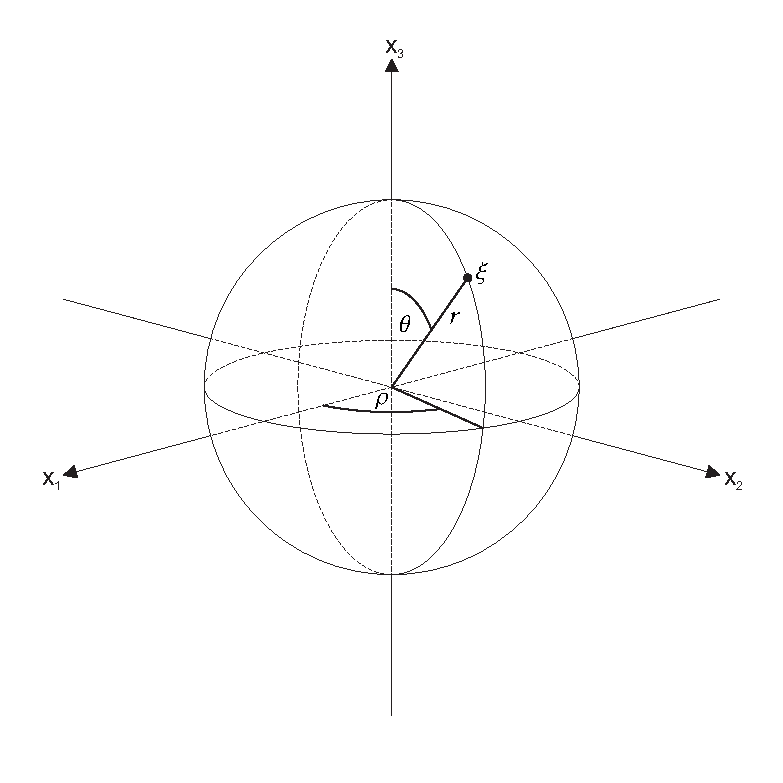
\includegraphics[height=12cm,width=12cm]{images/sphere}
  \caption{The spherical coordinate system in $\R^3$. Every point $\xi$ on a
  sphere with radius $r$ around the origin can be uniquely described by angles 
  $\vtheta$, $\vphi$ and the radius $r$. For $\vtheta = 0$ or
  $\vtheta = \pi$ the point $\xi$ coincides with the North or the South
  pole, respectively.}
  \label{sphere}
\end{figure}

\section{Legendre-type functions}
\label{Basics:LegendreTypeFunctions}
In this section we shortly define \emph{Legendre Polynomials}, \emph{associated Legendre functions} 
and \emph{associated Legendre polynomials} and collect some basic properties. These functions play 
a major role in Fourier analysis on the sphere and are key for the algorithms related to Fourier 
expansions developed in this text.

The Legendre polynomials $P_k : \interv{[}{-1}{1}{]} \rightarrow \R$, $k \in \N_{0}$ 
as classical orthogonal polynomials are given by their corresponding 
\emph{Rodrigues-formula}
\begin{equation}
  \nonumber
  \fun{P_k}{x} = \frac{1}{2^k k!} \frac{\dx^k}{\dx x^k} \paren{x^2-1}^k.
\end{equation}
The corresponding three-term recurrence relation is
\begin{equation}
  \nonumber
  \paren{k+1}\fun{P_{k+1}}{x} = \paren{2k+1}x\fun{P_{k}}{x} -
  k\fun{P_{k-1}}{x},\ k \in \N.
\end{equation}

Furthermore one defines the associated Legendre functions $P_k^n : \interv{[}{-1}{1}{]} \rightarrow \R$, 
$n \in \NZ$, $k=n,n+1,\ldots$ as 
\begin{equation}
  \nonumber
  \fun{P_k^n}{x} := \paren{\frac{\paren{k-n}!}{\paren{k+n}!}}^{1/2}
  \paren{1-x^2}^{n/2} \frac{\dx^n}{\dx x^n} \fun{P_k}{x}.
\end{equation}
For fixed $n$ the functions $\set{P_{k}^n}_{k=n,n+1,\ldots}$ form a complete set of orthogonal functions 
for $\Ln{2}{\interv{[}{-1}{1}{]}}$ with
$$ \frac{1}{2} \int_{-1}^{1} \fun{P_{k}^n}{x} \fun{P_{l}^n}{x} \dx x = \frac{1}{2k+1} \delta_{k,l}.$$
Furthermore, associated Legendre functions fulfill the recurrence relation
\begin{eqnarray*}
  & & \fun{P_{n-1}^n}{x} := 0,\qquad \fun{P_{n}^n}{x} = \frac{((2n)!)}{2^n n!}^{1/2} \paren{1-x^2}^{n/2},\\
  & & \fun{P_{k+1}^n}{x} = v_{k}^n x \fun{P_{k}^n}{x} + w_{k}^n \fun{P_{k-1}^n}{x} \quad (k = n,n+1,\ldots),
\end{eqnarray*}
where
$$ v_{k}^n := \frac{2k+1}{((k-n+1)(k+n+1))^{1/2}}\; ,\qquad w_{k}^n := - \frac{((k-n)(k+n))^{1/2}}{((k-n+1)(k+n+1))^{1/2}}\; .$$
A simple but at the same time very important idea is to define the associated Legendre functions also for 
$k < n$ by means of the three-term recurrence relation
$$ \fun{P_{k+1}^n}{x} = \paren{\alpha_{k}^n x \beta_{k}^n} \fun{P_{k}^n}{x} + \gamma_{k}^n \fun{P_{k-1}^n}{x} $$
with
\begin{eqnarray*}
  \alpha_{k}^n & := & \left\{
    \begin{array}{ll}
      (-1)^{k+1} & \text{for}\ k < n,\\
      v_{k}^n    & \text{otherwise},
    \end{array}\right.\\
  \beta_{k}^n & := & \left\{
    \begin{array}{lll}
      1 & \text{for}\ k < n,\\
      0 & \text{otherwise},
    \end{array}\right.\\
  \gamma_{k}^n & := & \left\{
    \begin{array}{lll}
      0       & \text{for}\ k \leq n,\\
      w_{k}^n & \text{otherwise.}
    \end{array}\right.\\
\end{eqnarray*}
For even $n$ one sets 
$$ \fun{P_{-1}^n}{x} := 0,\ \fun{P_{0}^n}{x} := \sqrt{\frac{(2n)!}{2^n n!}}$$
and for odd $n$
$$ \fun{P_{0}^n}{x} := \fun{P_{1}^n}{x} := \sqrt{\frac{(2n)!}{2^n n!}} \paren{1-x^2}^{1/2}$$
respectively. For $k >= n$ these functions coincide with the associated Legendre functions as defined above. 
As a matter of fact, $P_{k}^n$ is a polynomial of degree $k$ for even $n$ while $\paren{1-x^2}^{-1/2}P_{k}^n$
is a polynomial of degree $k-1$ for odd $n$.

Based on the recurrence coefficients from Equation \eqref{} and introducing a shift parameter $c \in \NZ$, one 
defines the associated Legendre polynomials $\fun{P_{k}^n}{\cdot,c}$ by
\begin{eqnarray*}
  & & \fun{P_{-1}^n}{x,c} := 0,\ \fun{P_{0}^n}{x,c} := 1,\\
  & & \fun{P_{k+1}^n}{x,c} = \paren{\alpha_{k+c}^n x + \beta_{k+c}^n} \fun{P_{k}^n}{x,c} + \gamma_{k+c}^n \fun{P_{k-1}^n}{x,c}
\end{eqnarray*}
By induction one verifies the relation between associated Legendre functions and polynomials in the following lemma.
\begin{lemma}
  Let the functions $P_{k}^n$ and $\fun{P_{k}^n}{\cdot,c}$ be given as in Equation \eqref{} and 
  Equation \eqref{} respectively. Then it holds
  $$ \fun{P_{c+k}^n}{x} = \fun{P_{k}^n}{x,c} \fun{P_{c}^n}{x} + \gamma_{c}^n \fun{P_{k-1}^n}{x,c+1} \fun{P_{c-1}^n}{x}. $$
\end{lemma}

\newpage

They can be characterized in ways similar
to those for Legendre polynomials, for instance by the
corresponding Rodrigues-formula or a differential equation. They
play an important role in the definition of spherical harmonics.
Note that for $k = 0$, the associated Legendre functions coincide with 
the Legendre polynomials.
Now let $k,m,n \in \N_0$, $k \le \min\encl{\{}{m,n}{\}}$. Then the associated
Legendre functions fulfill the orthogonality condition
\begin{equation}
\nonumber
  \int_{-1}^{1} \fun{P_{m}^{k}}{t} \fun{P_{n}^{k}}{t}\;dt =
  \frac{2}{2n+1}\delta_{m,n}.
\end{equation}


\section{Spherical Harmonics}
\label{Basics:SphericalHarmonics}

Spherical Harmonics on the sphere $\twosphere$ arise the same way as complex exponentials 
$e^{i k x}$ on the circle $\mathbb{S}^1$ and form a complete orthogonal system for $\Ln{2}{\twosphere}$.
Speaking of Fourier analysis with respect to the sphere, one refers to Spherical Harmonics as the Fourier 
Basis on $\twosphere$. In this section, we shortly introduce these basis functions mentioning basic properties.

From Laplace's differential equation $\Delta f = 0$ in $\R^3$, one obtains in spherical coordinates
\begin{equation}
  \label{SphericalHarmonics.LaplaceEquation.SphericalCoordinates}
  \Delta f = \frac{\partial^2 f}{\partial r^2} + \frac{2}{r}\frac{\partial f}{\partial
  r} + \frac{1}{r^2 \sin \vtheta}\frac{\partial}{\partial \vtheta}\paren{\sin \vtheta \cdot \frac{\partial f}{\partial
  \vtheta}} + \frac{1}{r^2 \sin \vtheta}\frac{\partial^2}{\partial \vphi^2} = 0.
\end{equation}
Using an ansatz based on separation of variables and taking into account that $r = 1$ when restricting the 
equation to $\twosphere$, one obtains the solutions
\begin{eqnarray*}
    & & Y_{k}^n: \interv{[}{0}{\pi}{]}\times\interv{[}{0}{2\pi}{)} \rightarrow
    \C,\ n \in \NZ,\; k = -n,-n+1,\ldots,n,\\
    & & \fun{Y_{k}^n}{\vtheta,\vphi} := \sqrt{\frac{2n+1}{4\pi}} 
    \fun{P_{k}^{\abs{n}}}{\cos \vtheta} e^{in\vphi}.
\end{eqnarray*}
Figure \ref{Basics:SphericalHarmonics} shows the absolute value of some of the 
functions $Y_{k}^{n}$. An important result is that these functions all are contained in $\fun{\text{Harm}_n}{\twosphere}$.
Due to the separability one proves easily that they also fulfill the orthogonality condition with respect 
to the standard scalar product on $\twosphere$:
\begin{equation}
  \nonumber
  \scalarproduct{Y_{k}^n}{Y_{l}^m}_{\twosphere} = \delta_{k,k} \delta_{n,m}
\end{equation}
No let $\mathcal{H}_k$ denote
$\text{Harm}_k\paren{\twosphere}$, then
for every $k \in \NZ$, the set
\begin{equation}
  \nonumber
  \pset{Y_{k}^n}{|}{n = -k,-k1+1,\ldots,k}
\end{equation}
forms an orthonormal basis of $\mathcal{H}_k$, since $\dim \mathcal{H}_k =
2k+1$. Moreover, the spaces $\mathcal{H}_k$ are orthogonal
to each other and the set 
$$\pset{Y_{k}^n}{|}{k = 0,1,\ldots,K,\ n = -k,-k+1,\ldots,k},\ K \in \NZ$$ 
provides an orthonormal basis for the space $\bigoplus_{k=0}^{K}\mathcal{H}_k$ called
the space of \emph{spherical harmonics} of degree $K$.

At first glance, the restriction to homogeneous and harmonic polynomials
might exclude various functions from being as well representable
as in $\fun{\Pol_K}{\twosphere}$. But as a matter of fact these
spaces are identical, i.e. 
\begin{equation}
  \nonumber
    \fun{\Pol_K}{\twosphere} = \bigoplus_{k=0}^{K}\mathcal{H}_k.
\end{equation}

\begin{figure}[htbp]
  \label{Basics:SphericalHarmonics}
  \centering
   \subfigure[$\abs{Y_{0}^{0}}$]
     {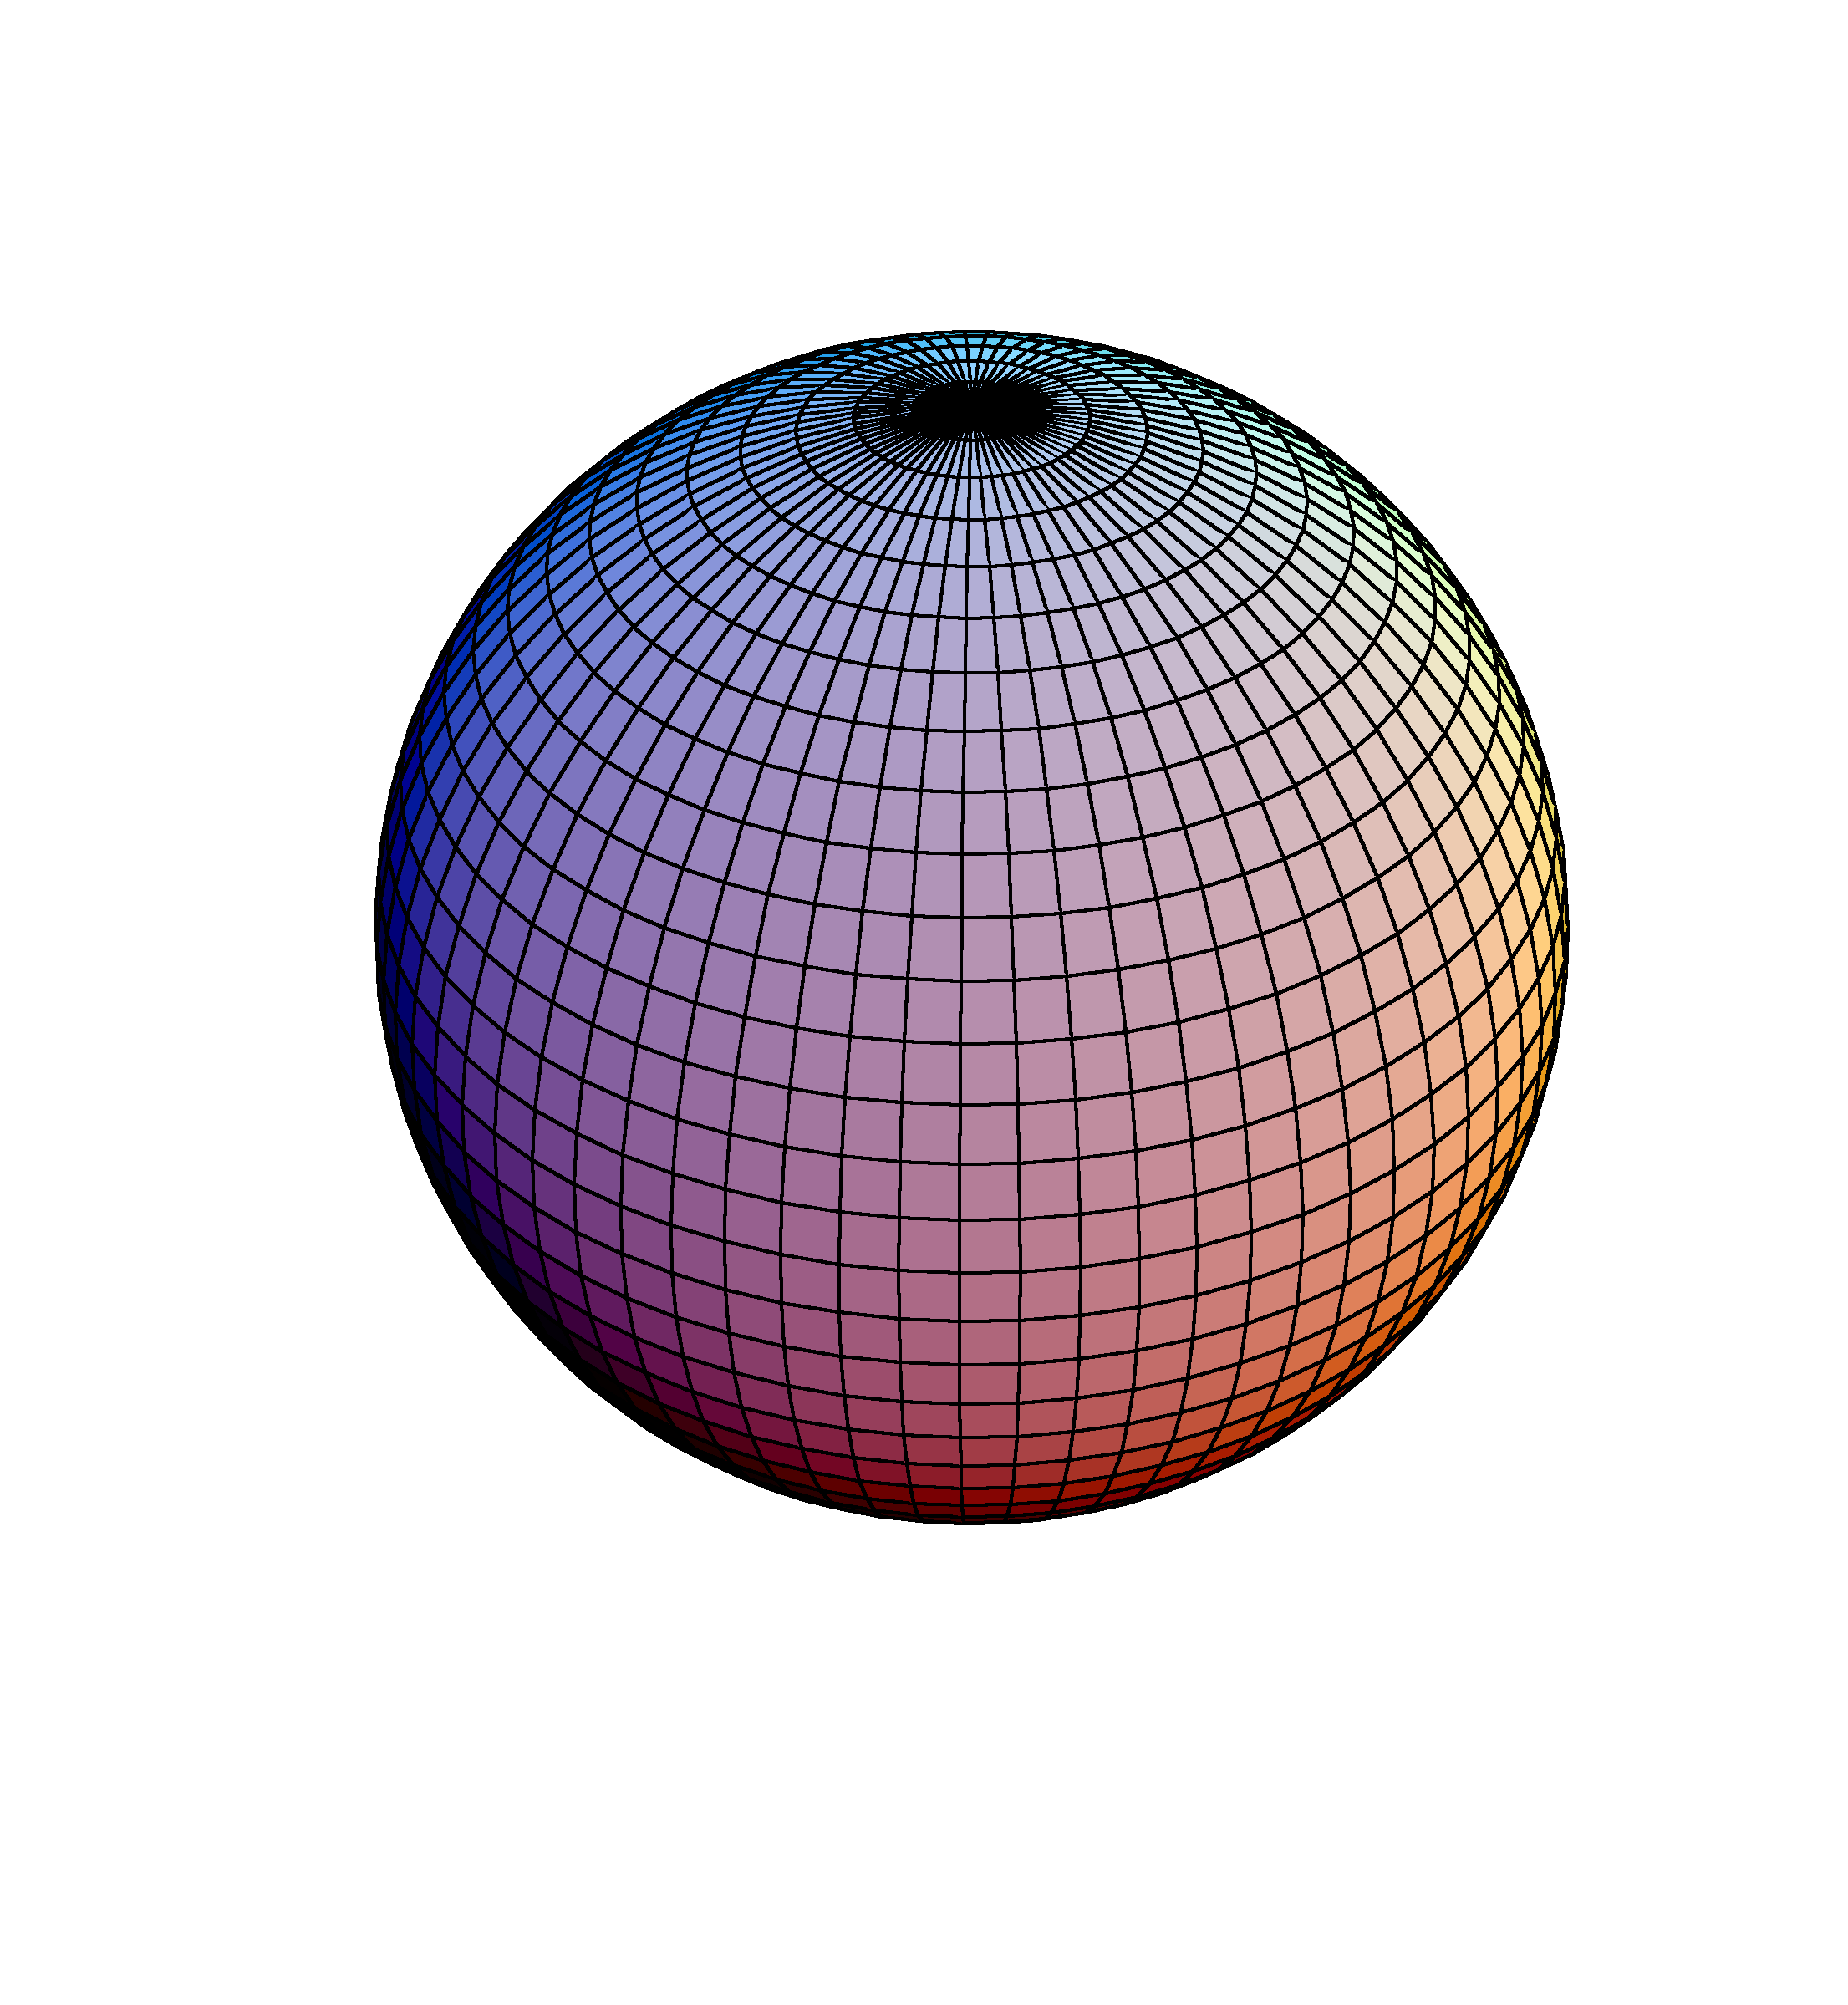
\includegraphics[width=0.3\textwidth]{images/sh_0_0.png}}\hfill
   \subfigure[$\abs{Y_{1}^{-1}}$]
     {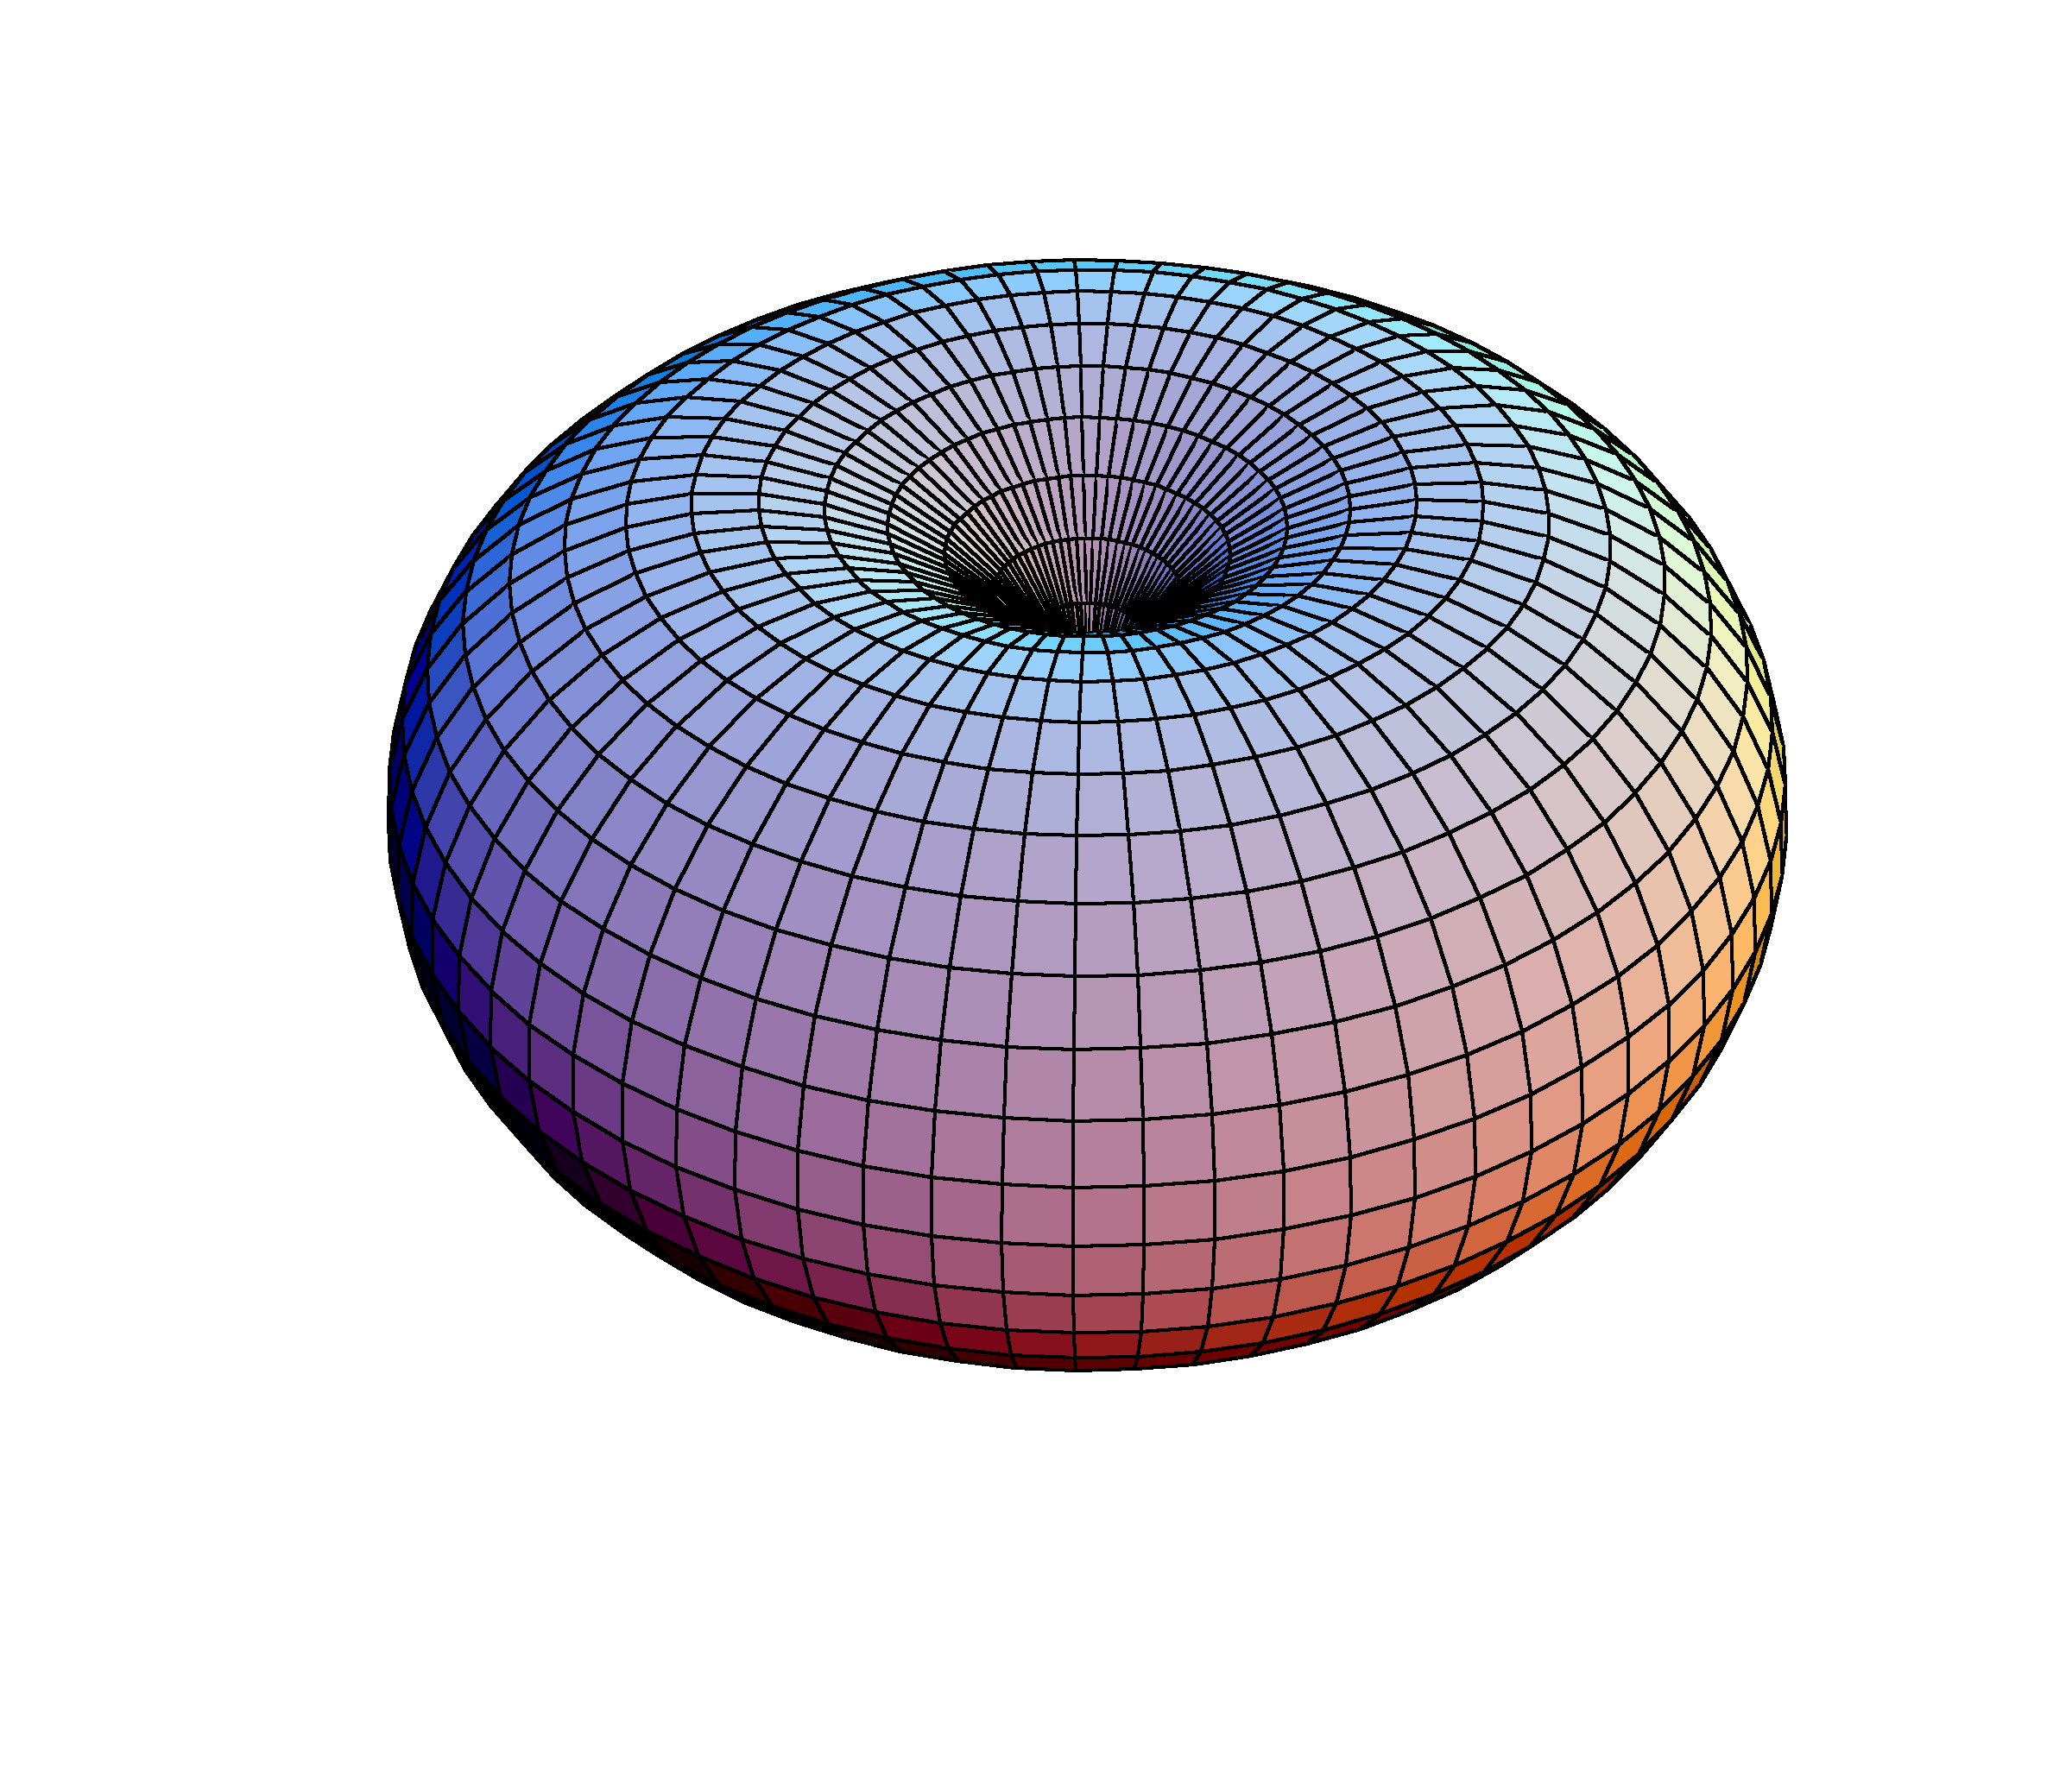
\includegraphics[width=0.3\textwidth]{images/sh_1_-1.png}}\hfill
   \subfigure[$\abs{Y_{1}^{0}}$]
     {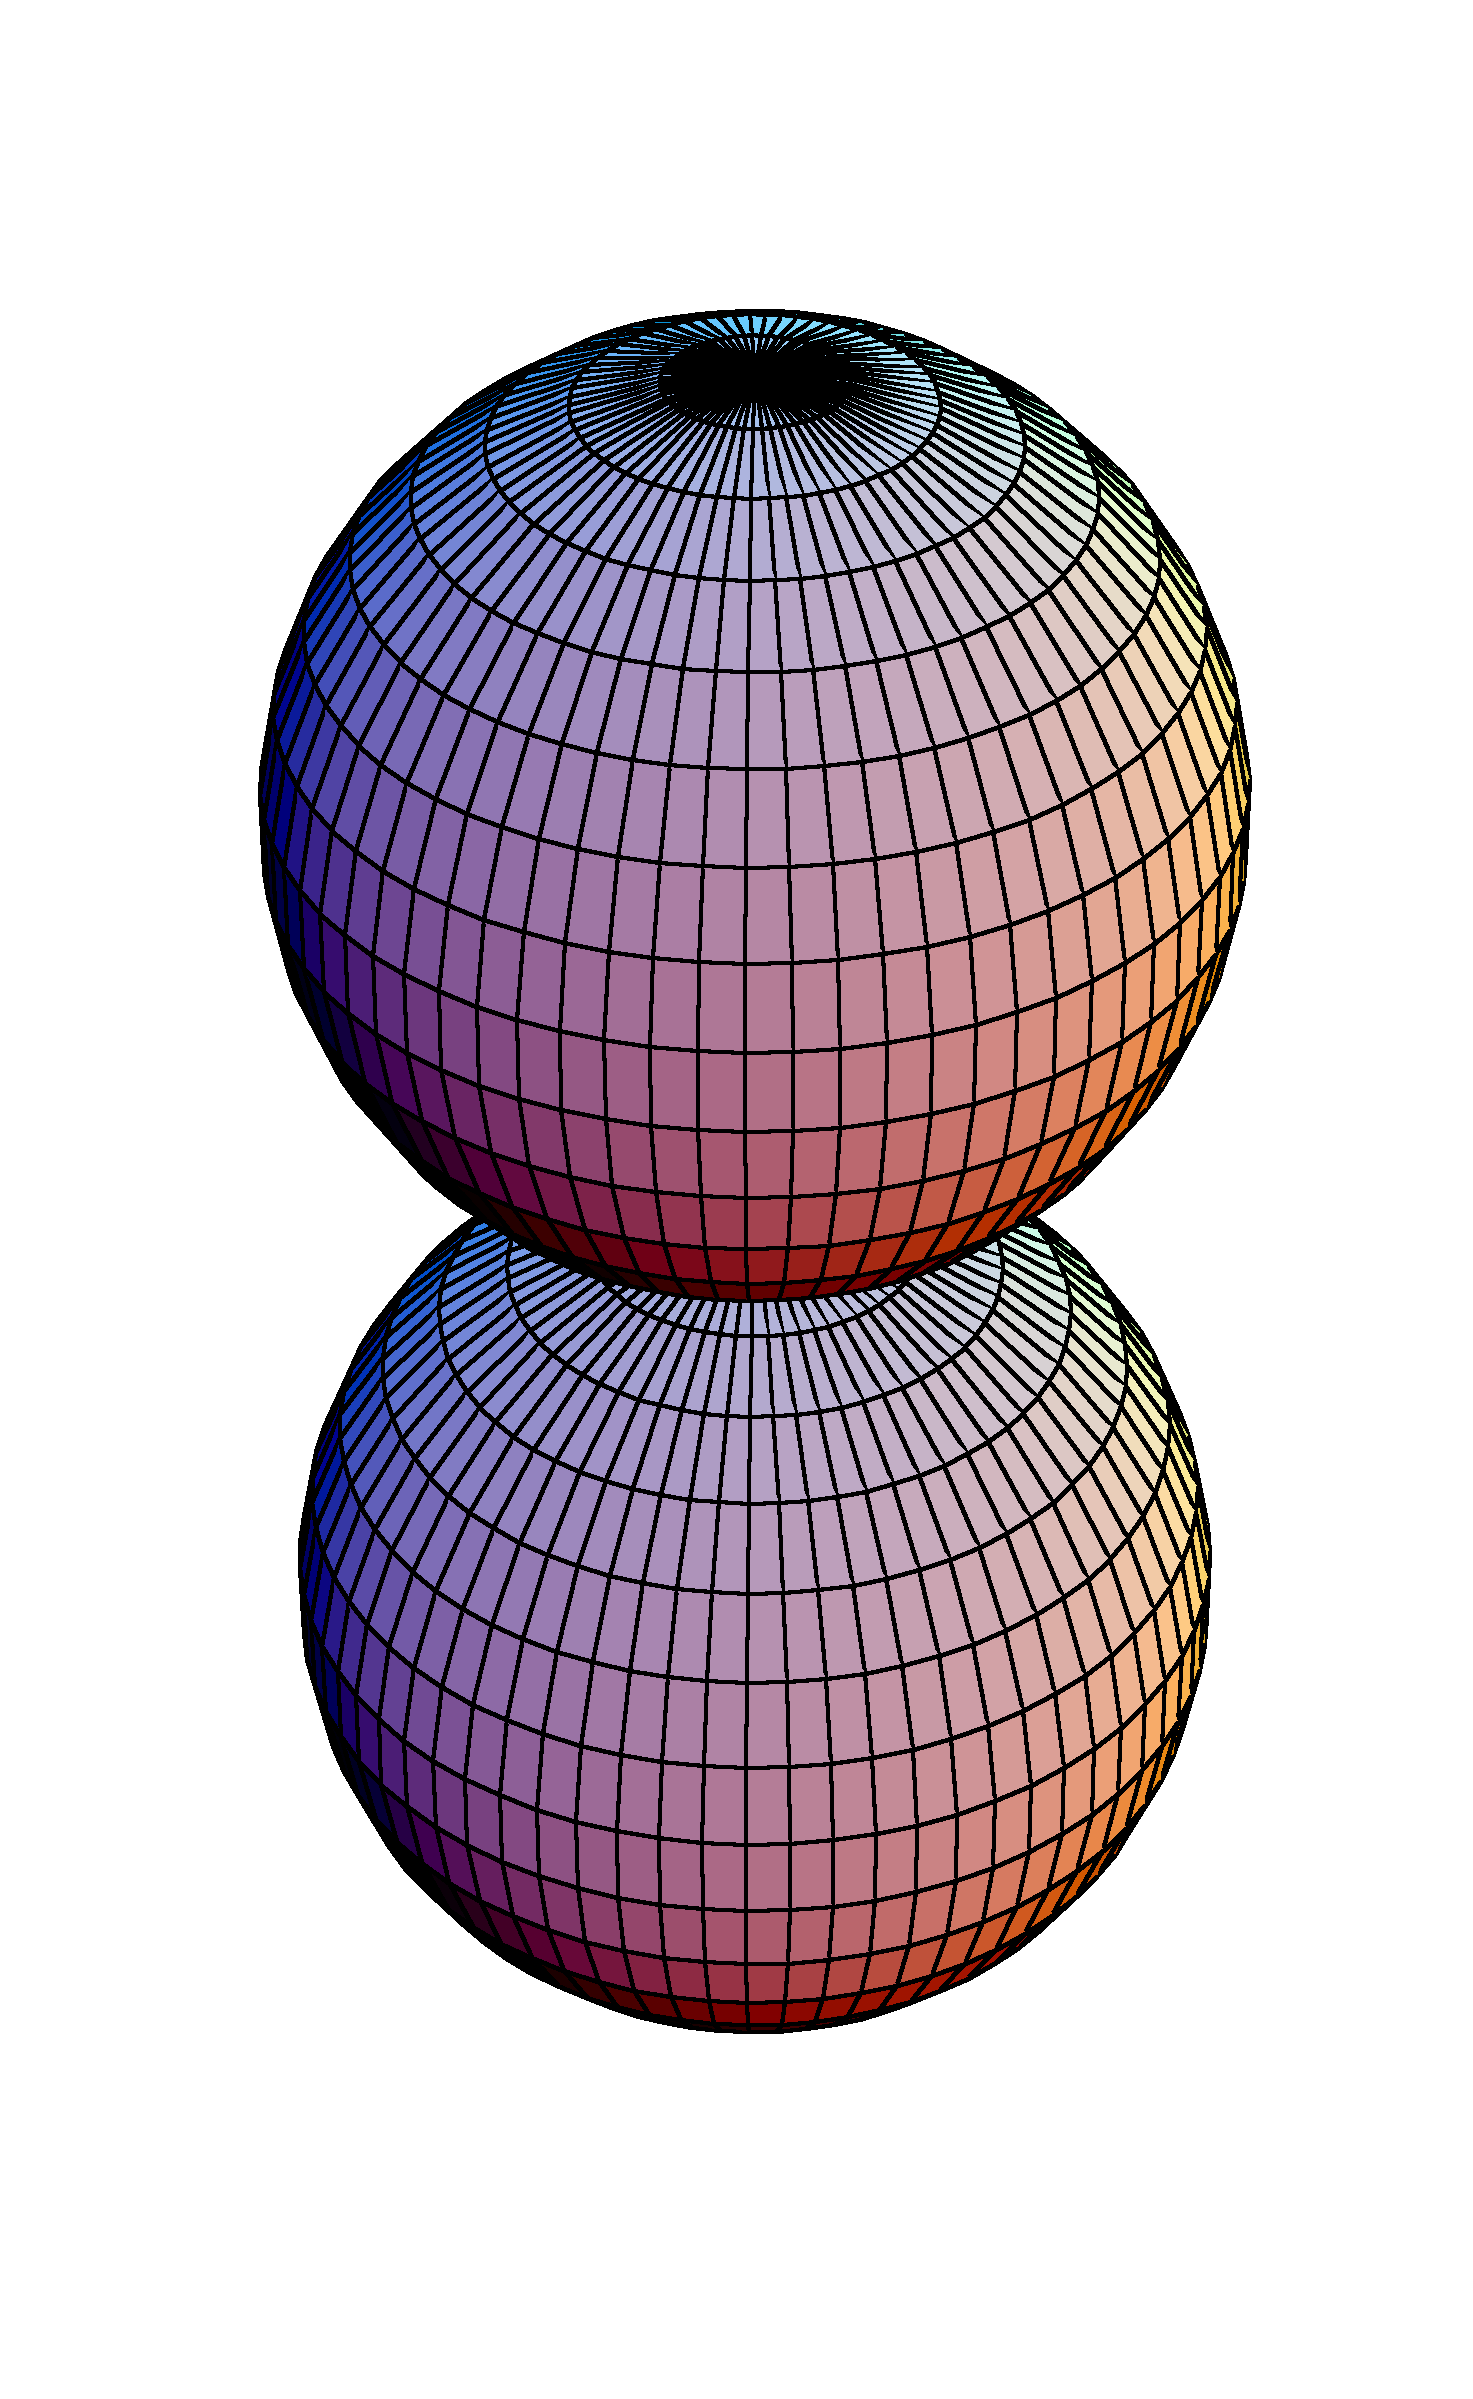
\includegraphics[width=0.3\textwidth]{images/sh_1_0.png}}\\
   \subfigure[$\abs{Y_{1}^{1}}$]
     {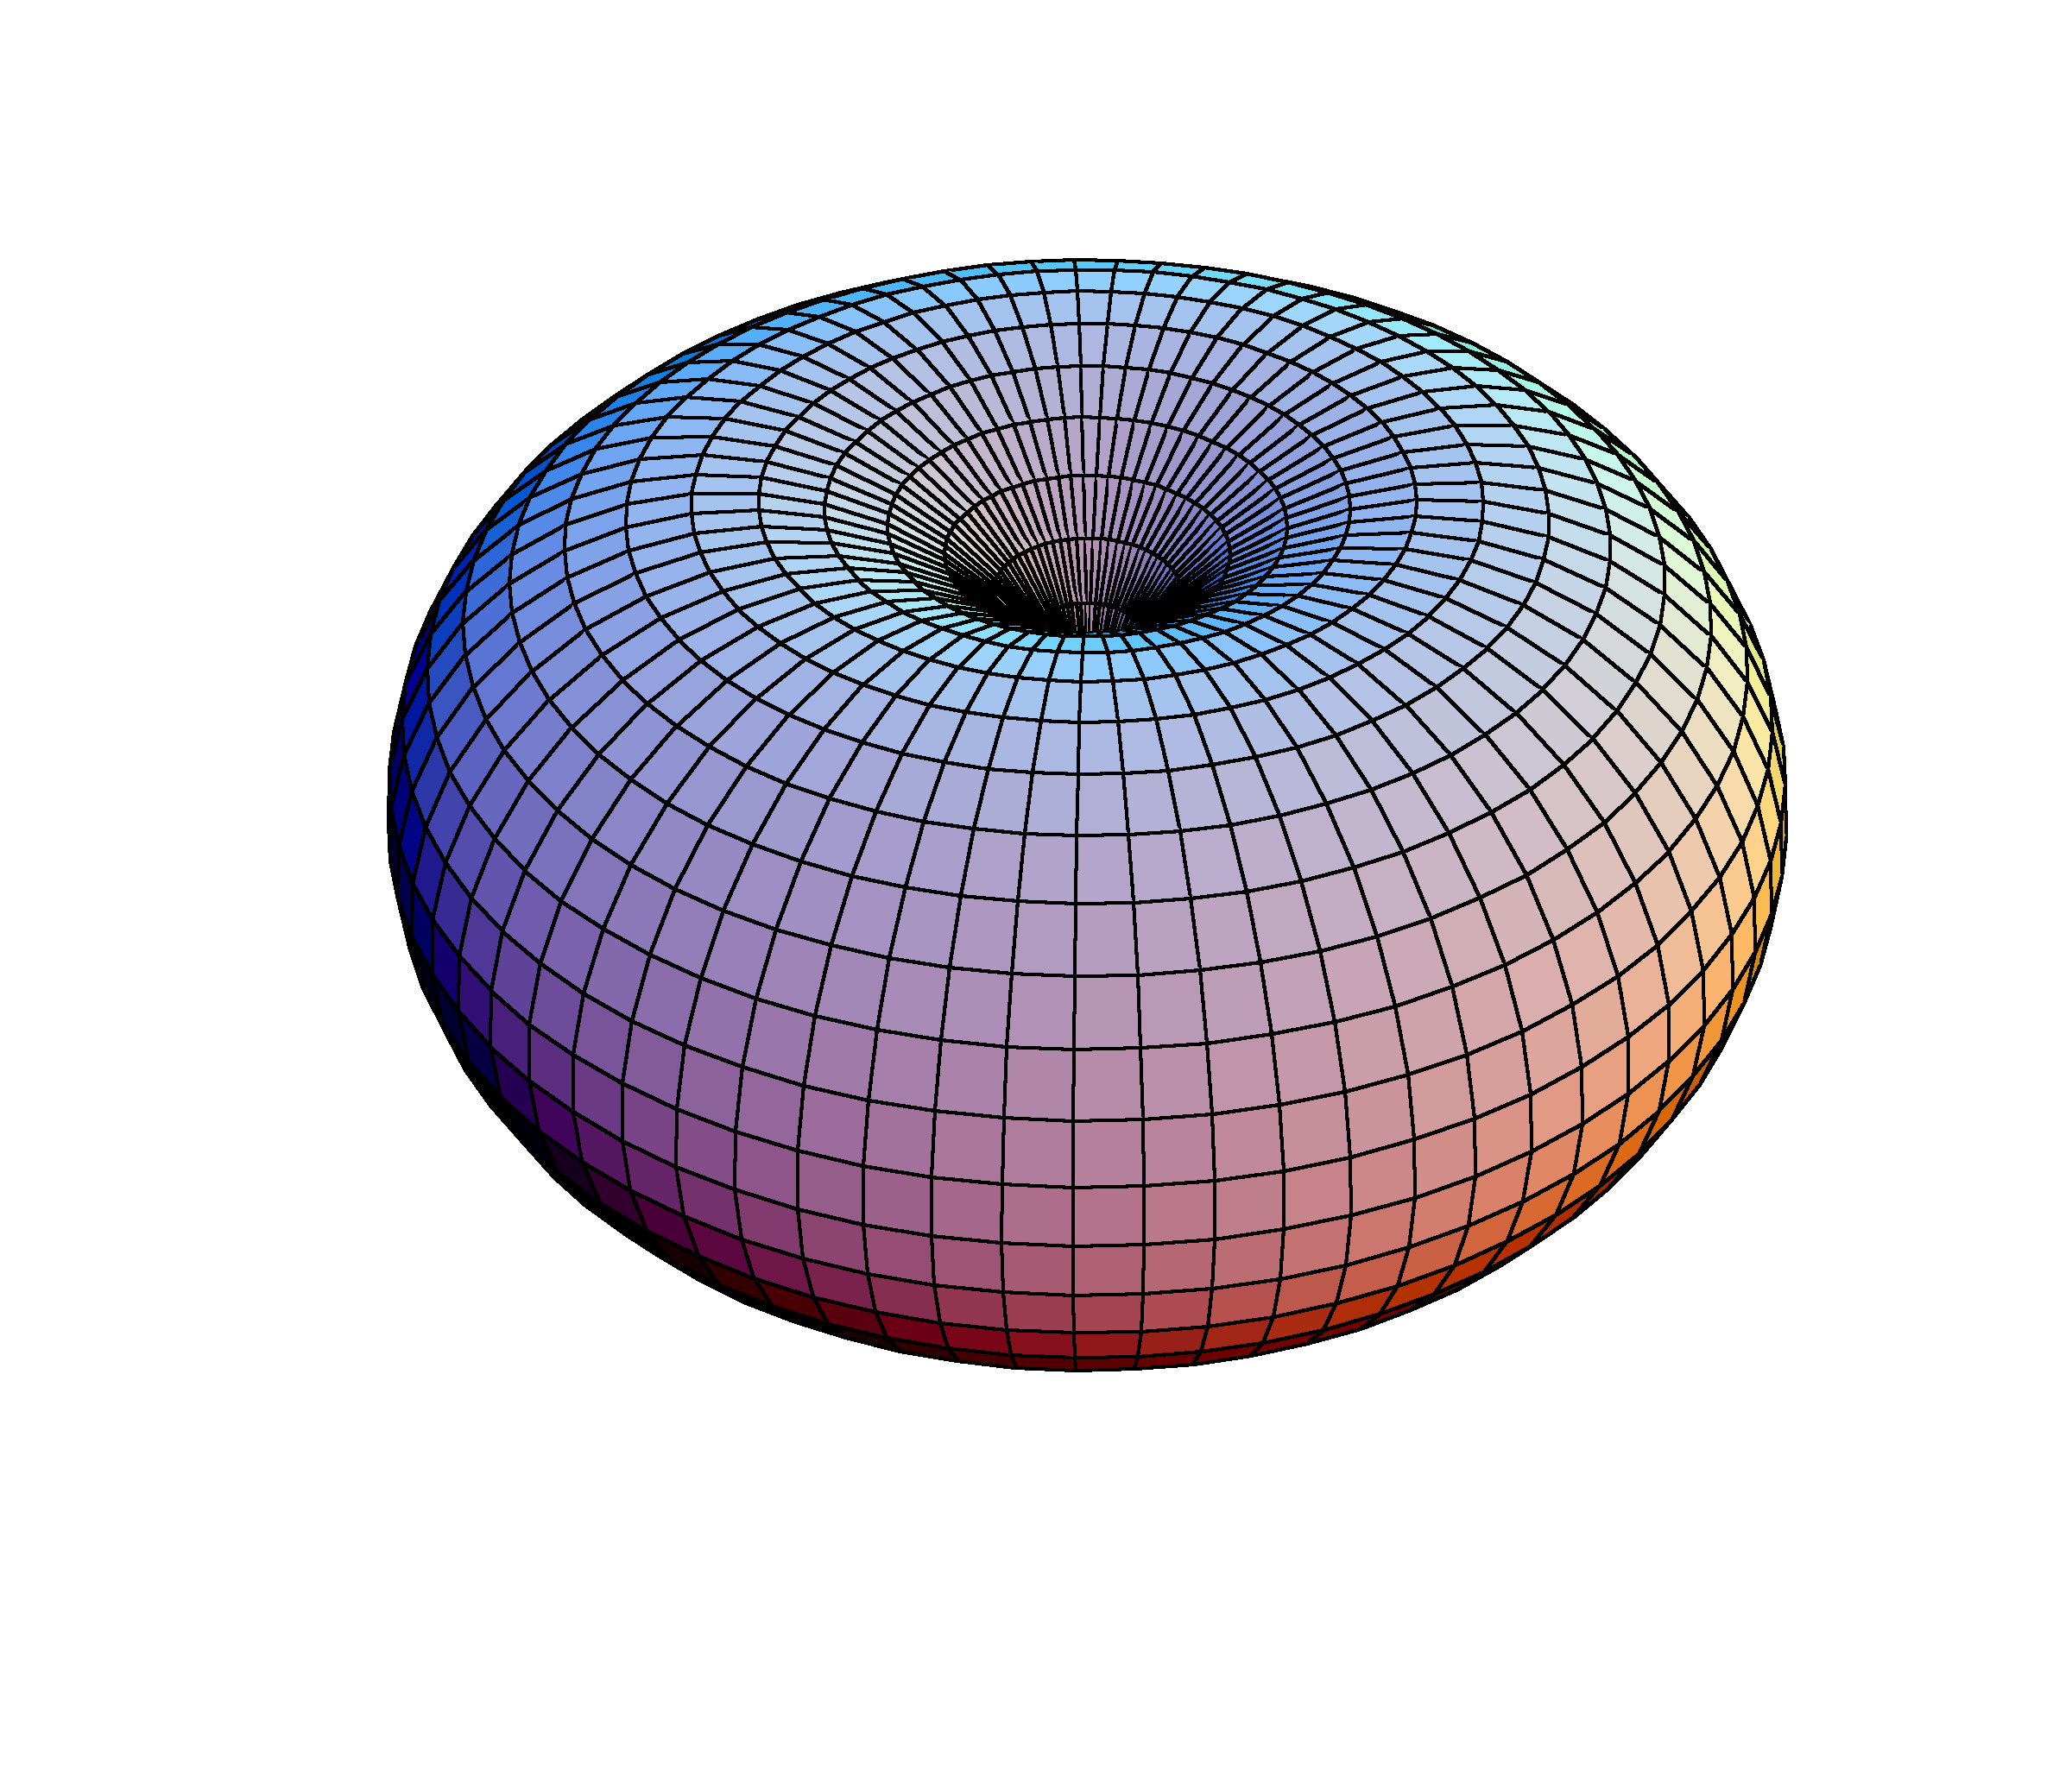
\includegraphics[width=0.3\textwidth]{images/sh_1_1.png}}\hfill
   \subfigure[$\abs{Y_{2}^{-2}}$]
     {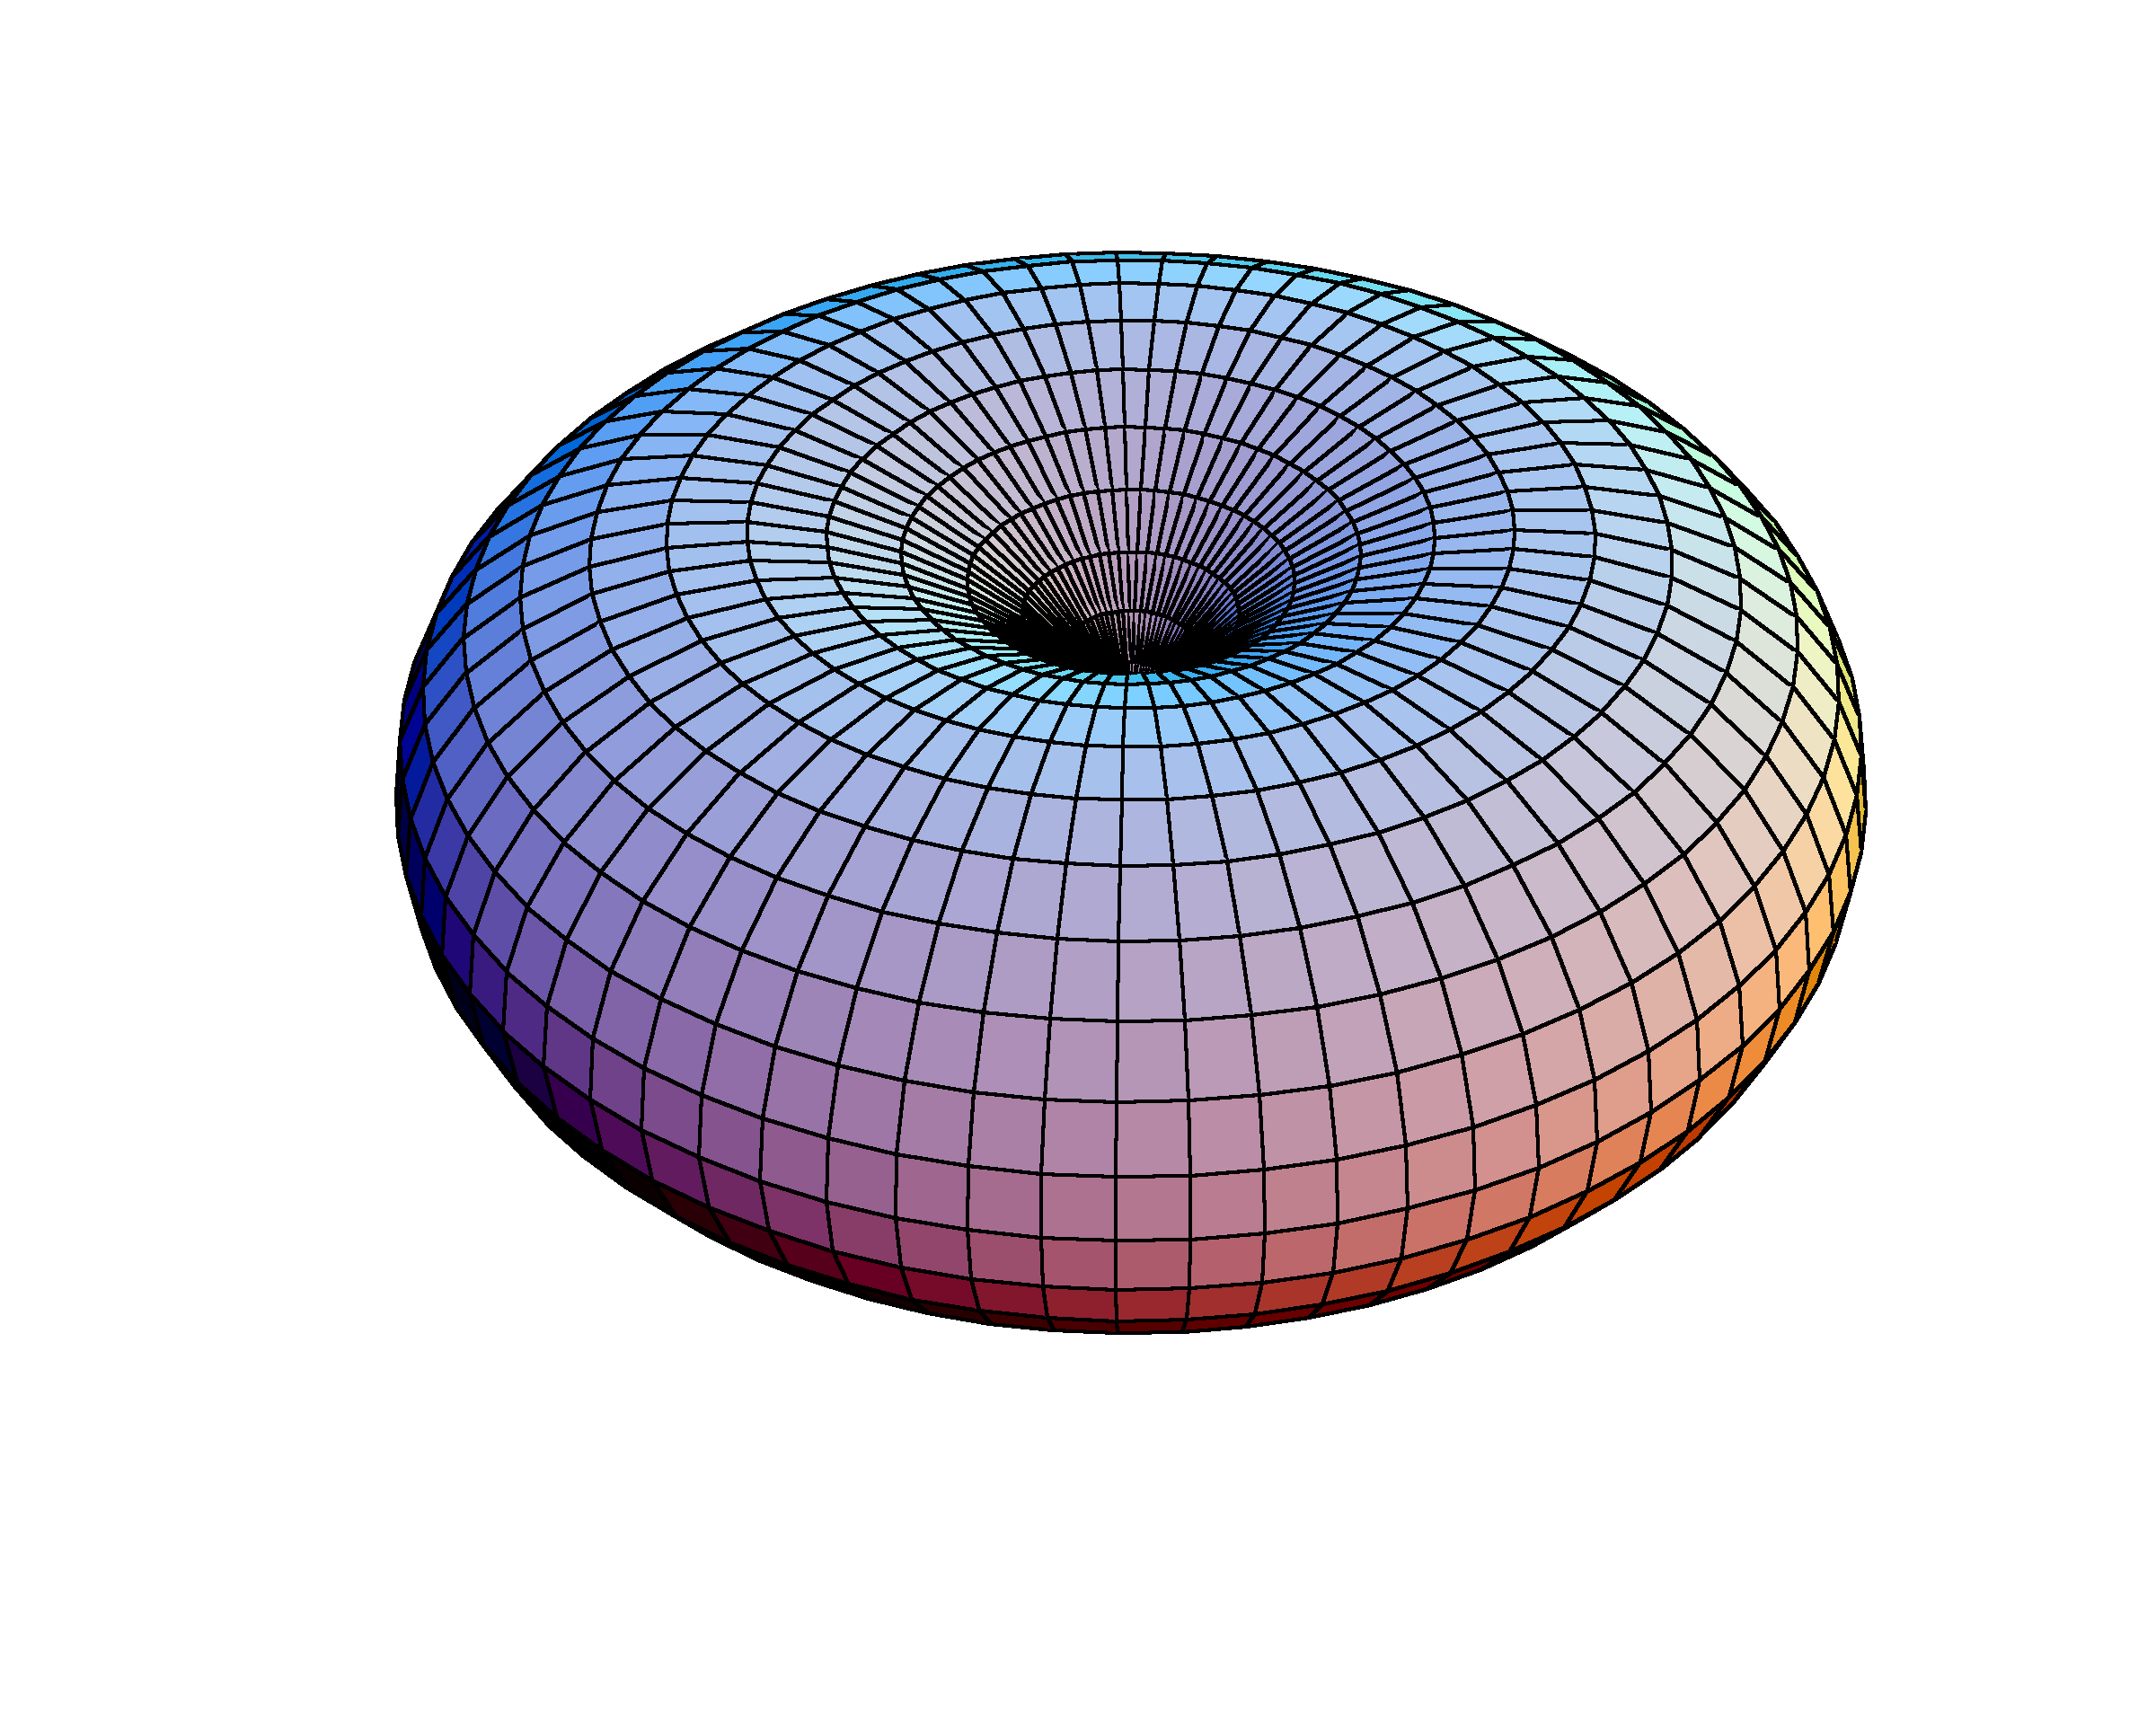
\includegraphics[width=0.3\textwidth]{images/sh_2_-2.png}}\hfill
   \subfigure[$\abs{Y_{2}^{-1}}$]
     {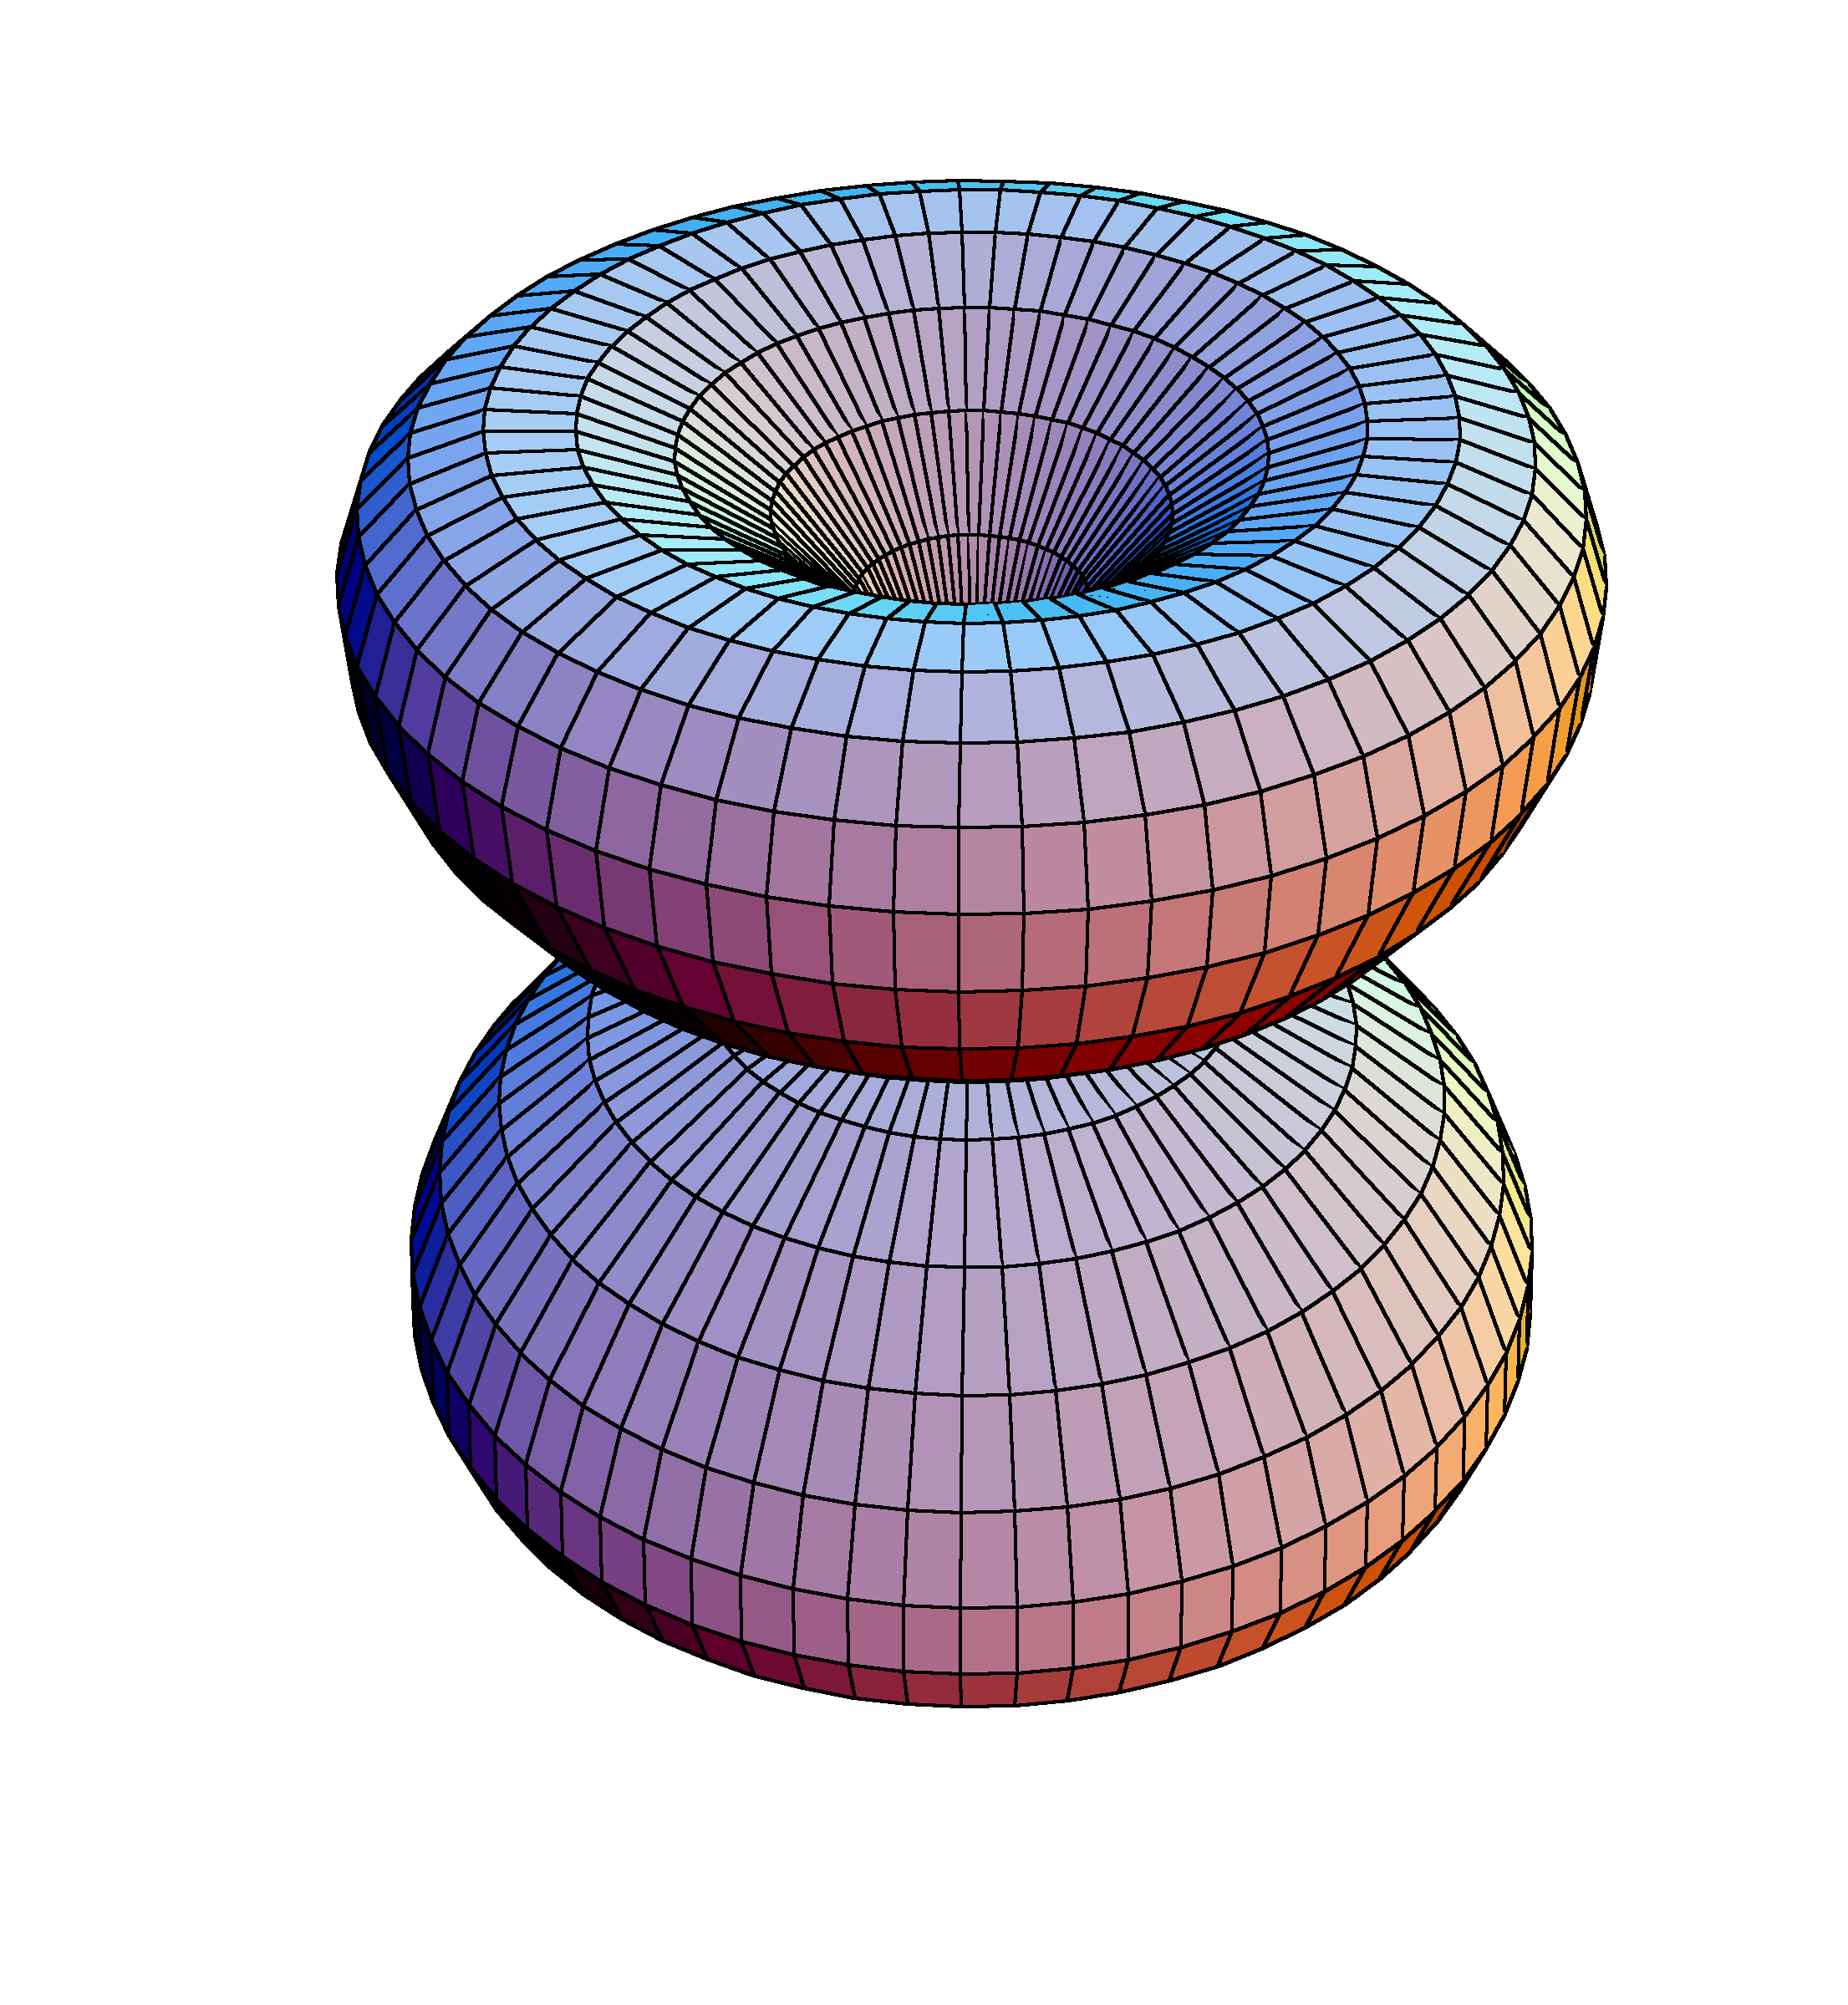
\includegraphics[width=0.3\textwidth]{images/sh_2_-1.png}}\\
   \subfigure[$\abs{Y_{2}^{0}}$]
     {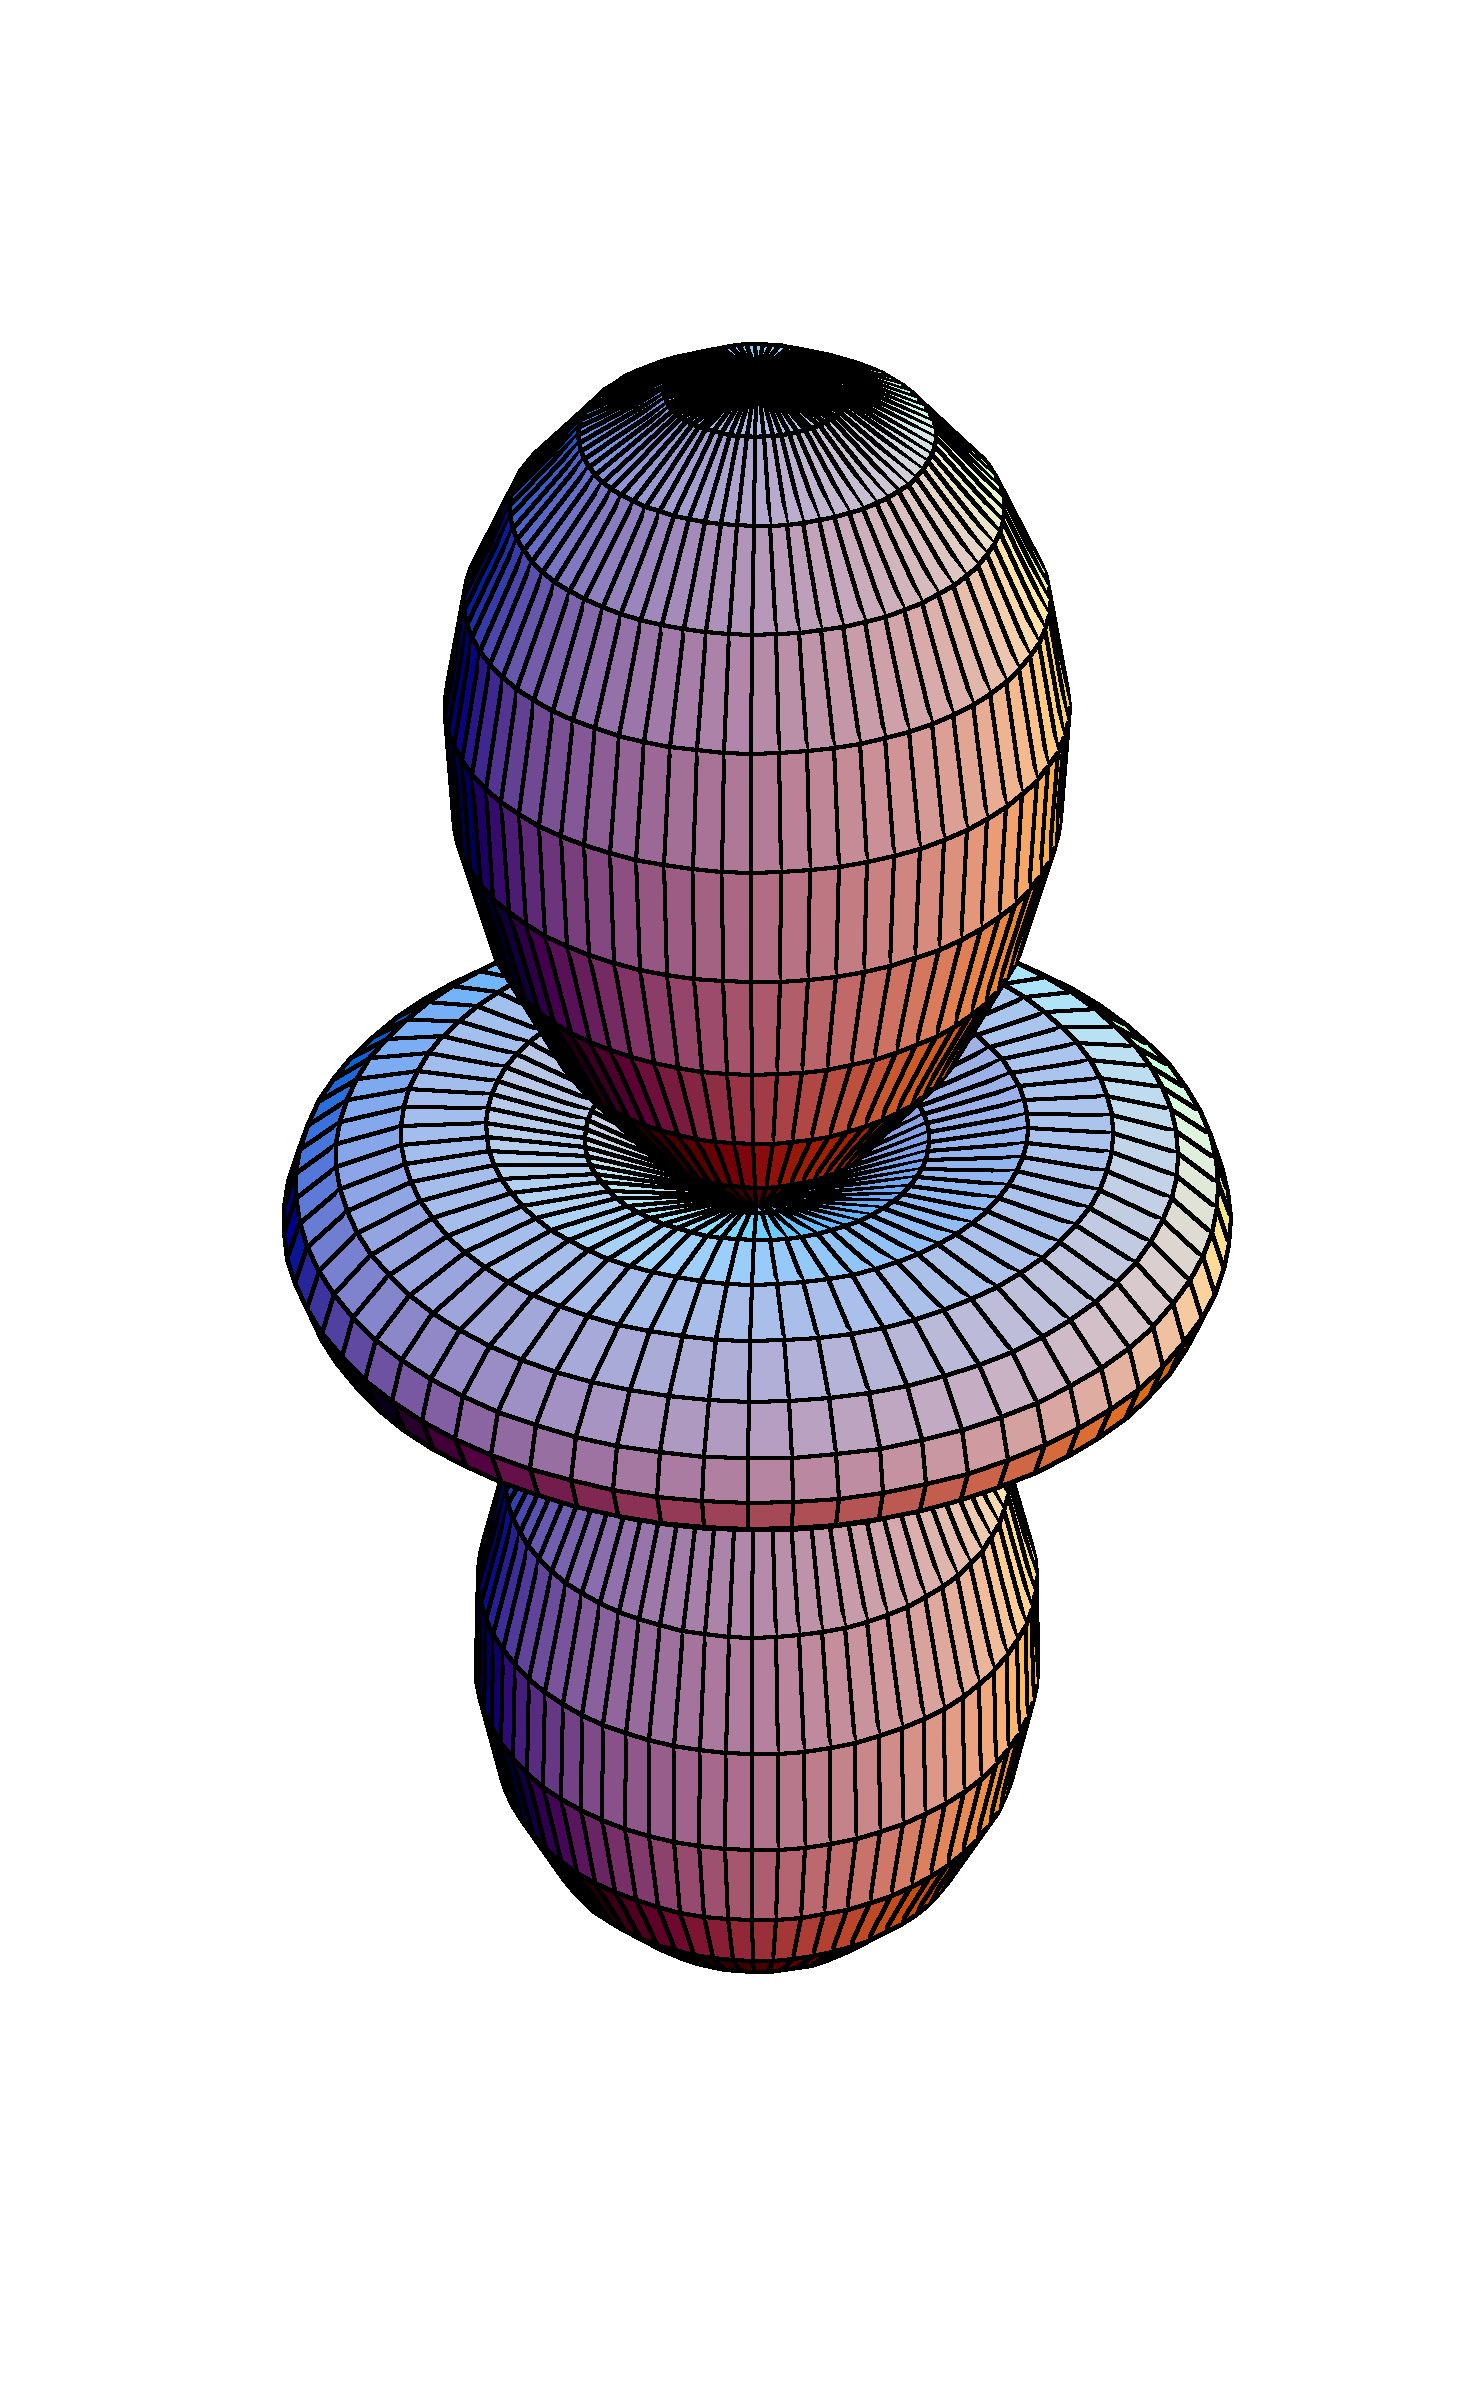
\includegraphics[width=0.3\textwidth]{images/sh_2_0.png}}\hfill
   \subfigure[$\abs{Y_{2}^{1}}$]
     {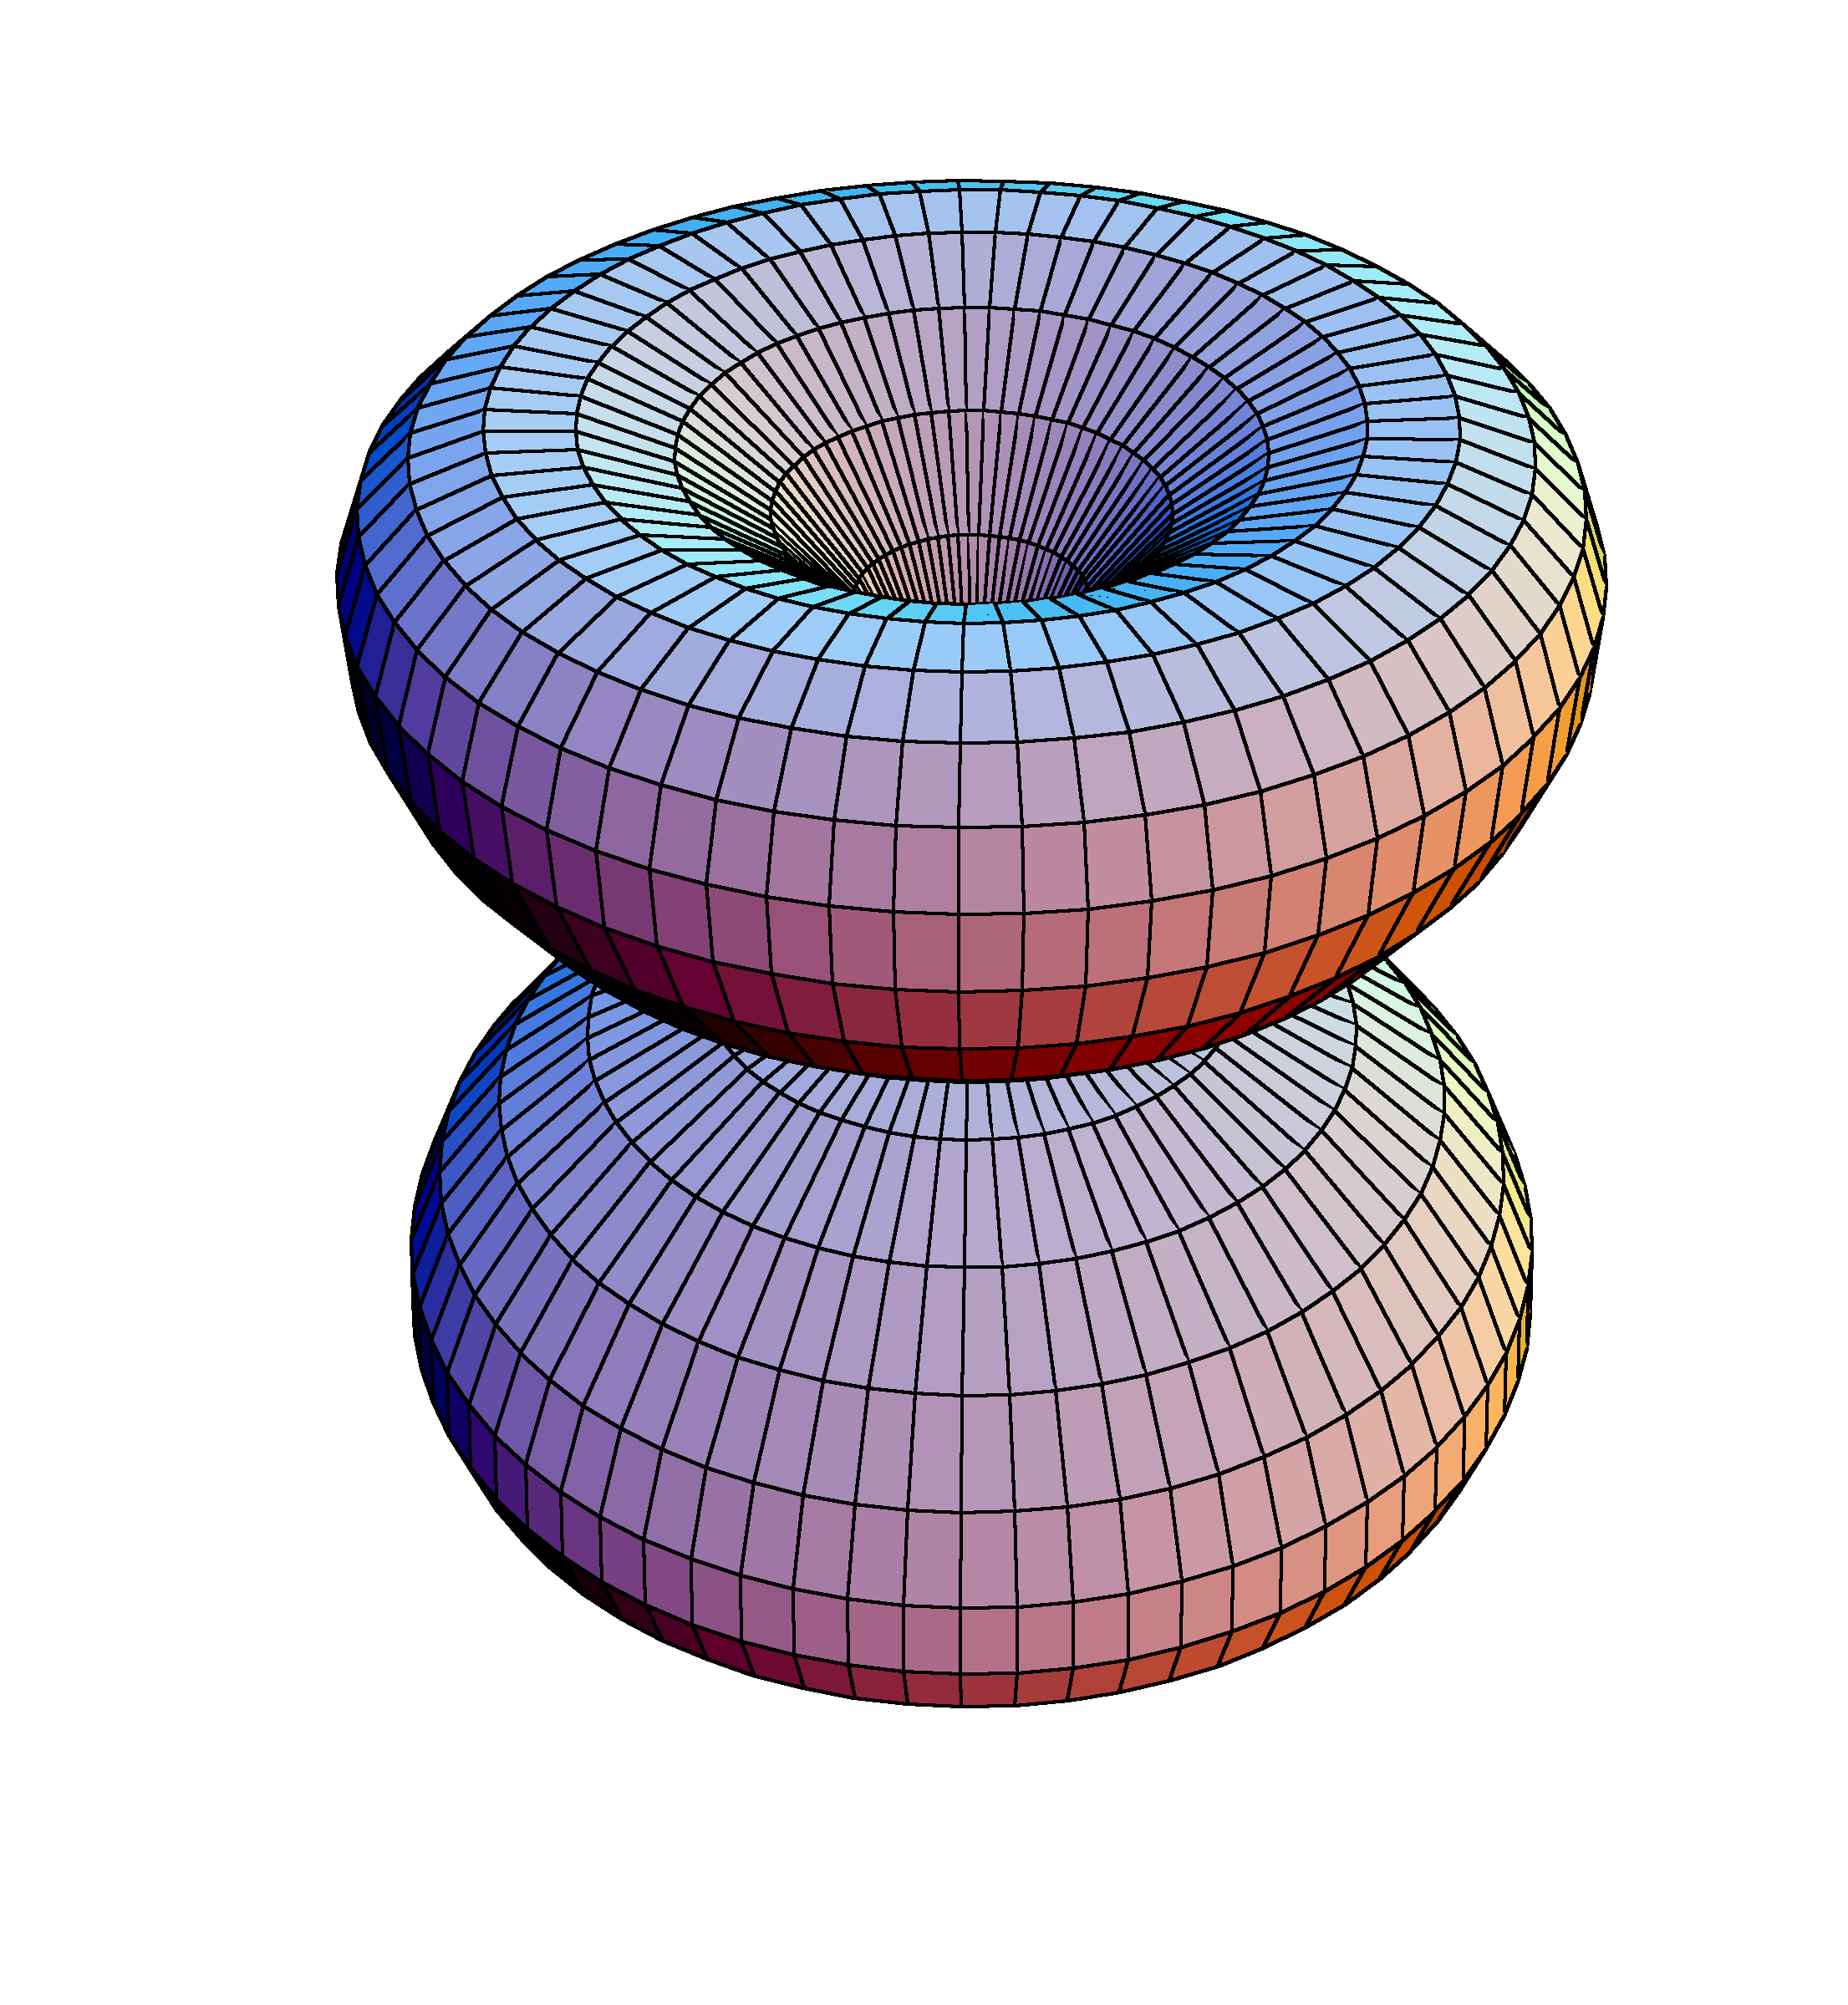
\includegraphics[width=0.3\textwidth]{images/sh_2_1.png}}\hfill
   \subfigure[$\abs{Y_{2}^{2}}$]
     {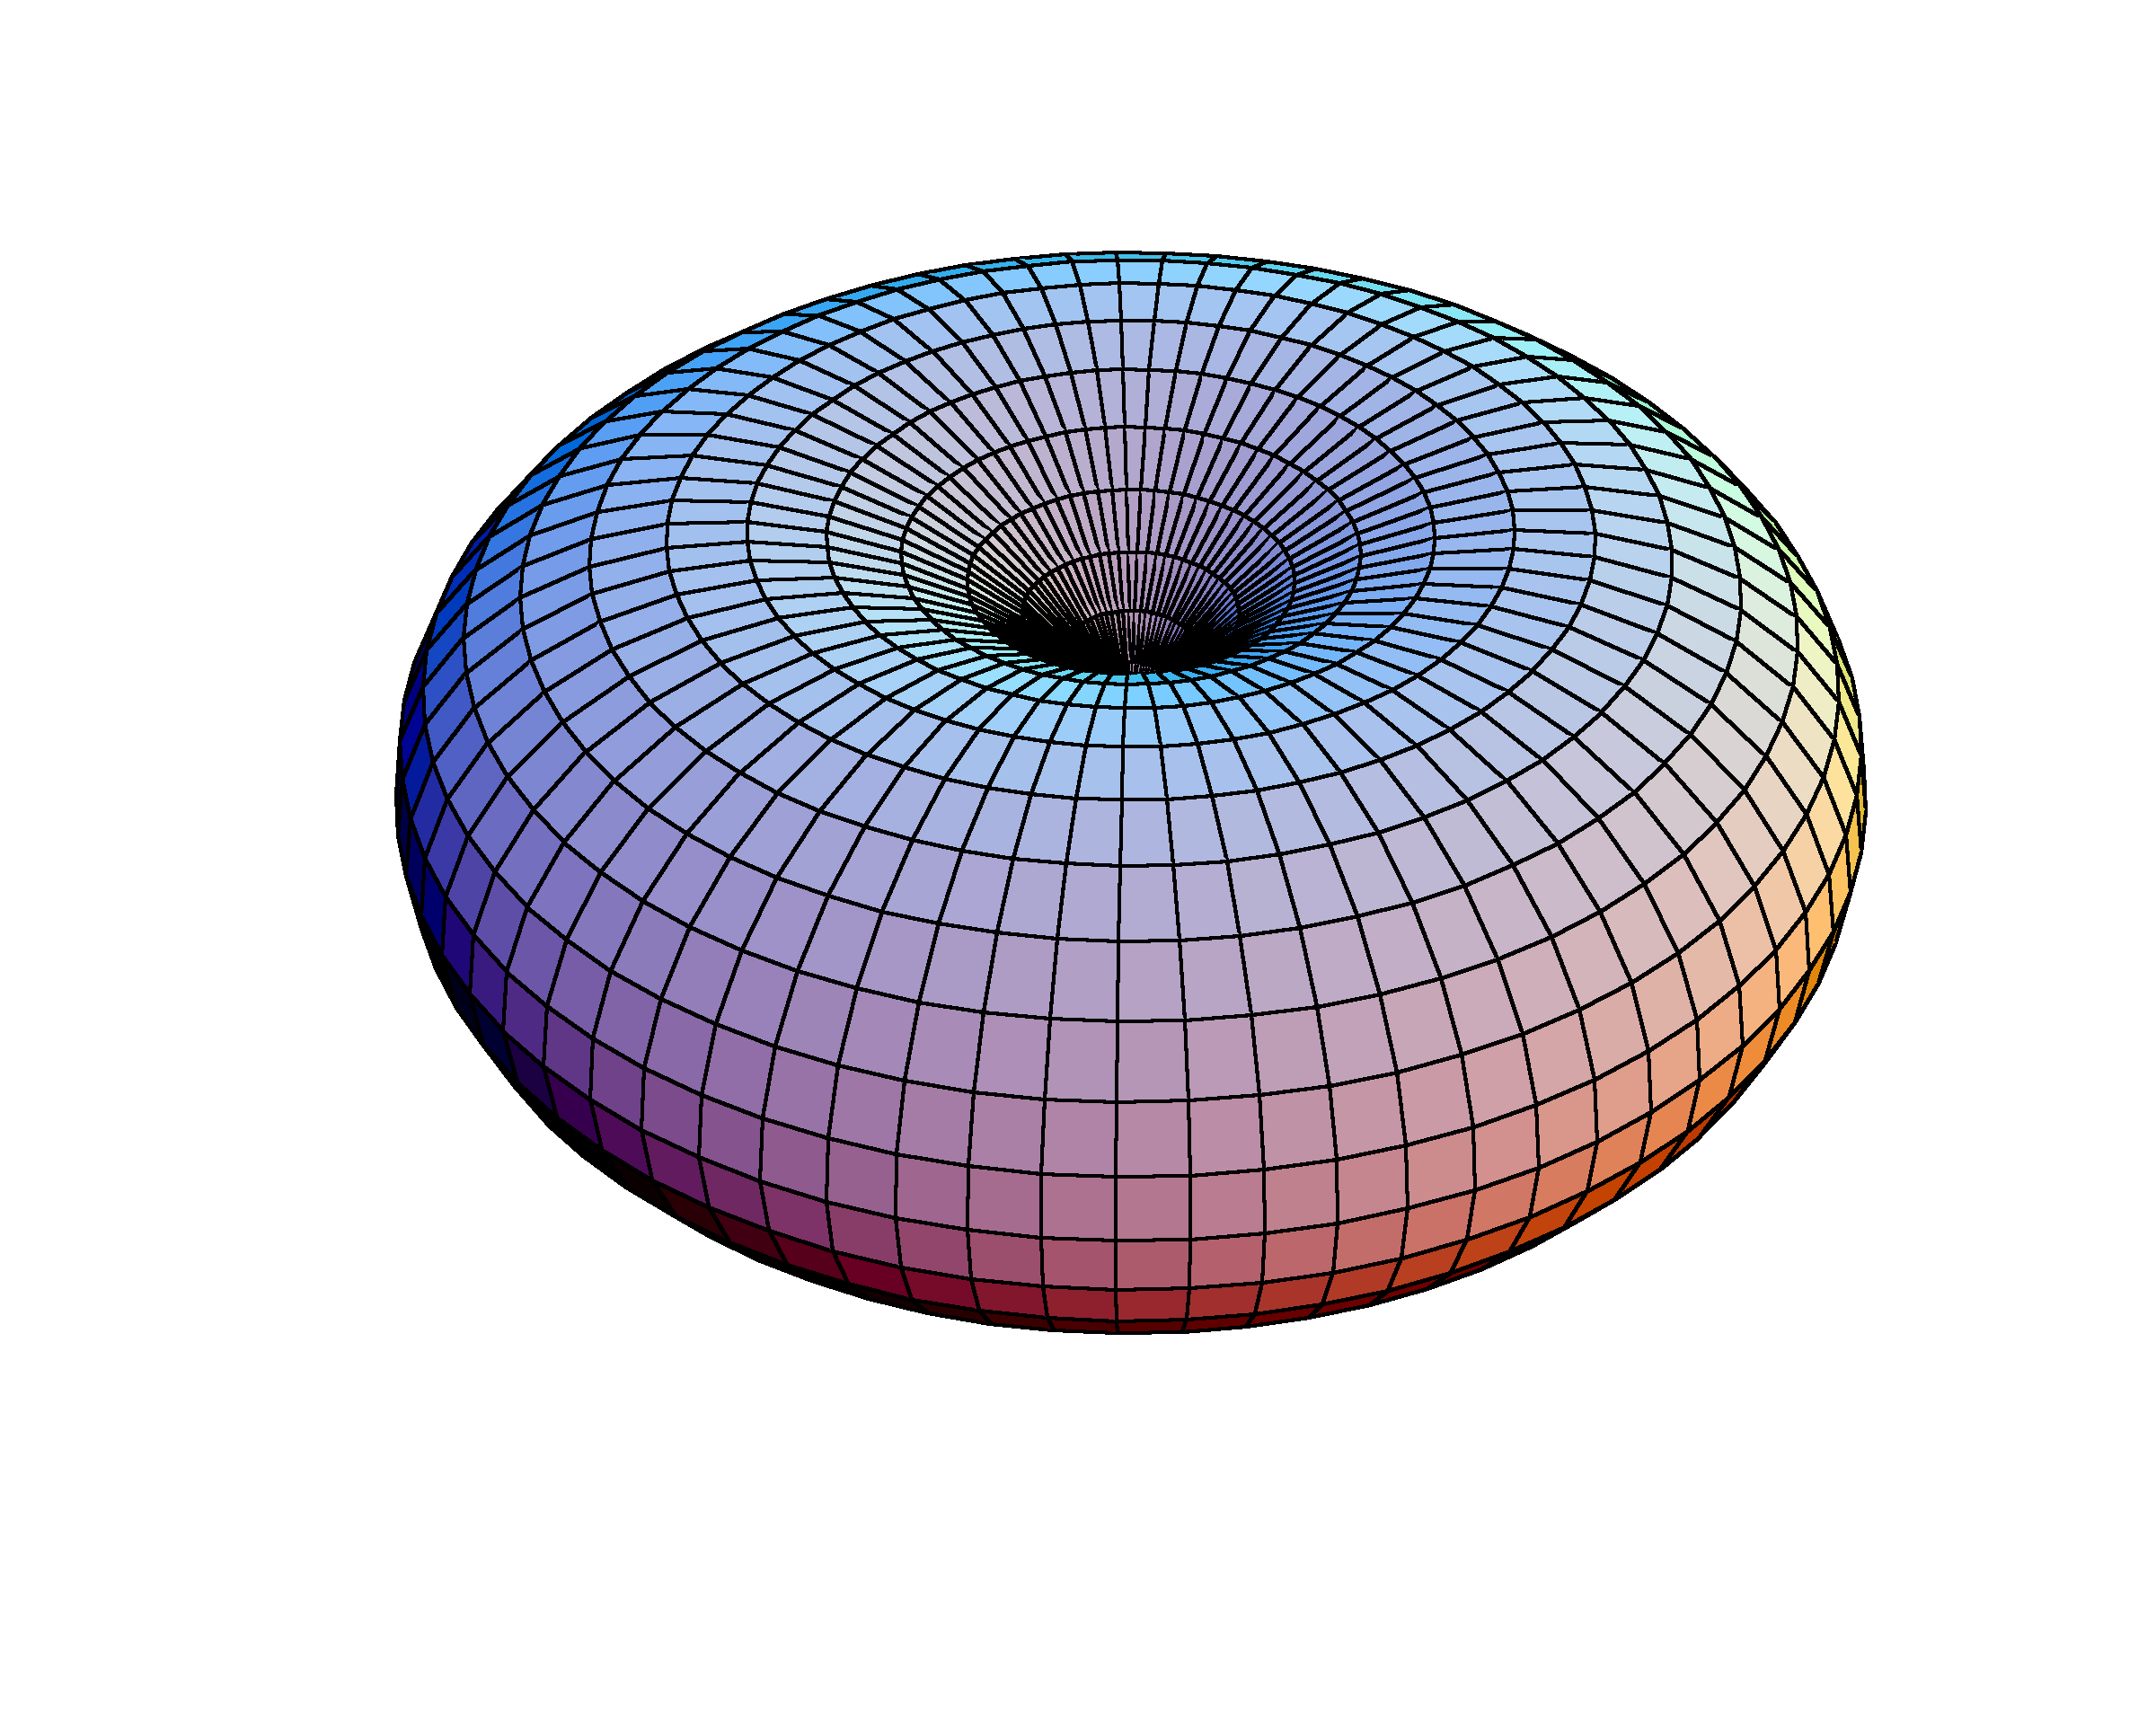
\includegraphics[width=0.3\textwidth]{images/sh_2_2.png}}\\
  \caption{To be written...}
\end{figure}

Finally, we mention the well known addition theorem for spherical harmonics 
that relates functions $Y_k^n$ forming an orthonormal basis of $\mathcal{H}_n$ 
to the Legendre polynomials. It particularly holds for the basis as given above but
generally is also applicable to every orthonormal basis.

\begin{proposition}[Addition Theorem]
  \label{AdditionTheorem}
  For every $\fun{L^2}{\twosphere}$ orthonormal basis 
  $\set{Y_{n,k}}_{k=-n}^{n}$ of $\mathcal{H}_n$, it holds
  \begin{equation}
    \nonumber
    \sum_{n=-k}^{k} \fun{Y_{k}^n}{\V{\xi}} \overline{\fun{Y_{k}^n}{\V{\eta}}} =
    \frac{2k+1}{4\pi}\fun{P_k}{\scalarproduct{\V{\xi}}{\V{\eta}}_{\twosphere}}.
  \end{equation}
\end{proposition}

\section{Radial Spherical Kernels}
A \emph{radial spherical kernel} is a radial symmetric function defined on the sphere. 
Generally, one starts with a continuous function $G: \interv{[}{-1}{1}{]} \rightarrow \C$ and defines 
for a fixed $\V{\eta} \in \twosphere$ a kernel function $K_{\V{\eta}}: \twosphere \rightarrow \C$ by
$$ \fun{K_{\V{\eta}}}{\cdot} := \fun{G}{\scalarproduct{\eta}{\V{\cdot}}_{\twosphere}}.$$
The function $G$ can be developed into a series of Legendre polynomials
$$ \fun{G}{x} = \sum_{k = 0}^{\infty} a_k \fun{P_k}{x}$$
where the coefficients $a_k$ are the scalar products
$$ a_k = \int_{-1}^{1} \fun{G}{x} \fun{P_k}{x} \dx x.$$
Applying the Addition Theorem from Proposition \ref{AdditionTheorem}, one gets the kernel 
representation
$$\fun{K_{\V{\eta}}}{\cdot} = \sum_{k = 0}^{\infty} a_k \fun{P_k}{\scalarproduct{\V{\eta}}{\cdot}_{\twosphere}} =  
\sum_{k = 0}^{\infty} a_k \frac{4\pi}{2k+1} \sum_{n=-k}^k \fun{Y_{k}^n}{\V{\xi}} \overline{\fun{Y_{k}^n}{\V{\eta}}}.$$
One is often interested in evaluating such an expansion on the sphere in a fast way when dealing with 
spherical convolution. As an application of the algorithms developed in this text, one can derive 
an algorithm based on the discrete spherical Fourier transform, as shown in Chapter \ref{}.

As an example of a radial spherical kernel function, we consider the generating series of the Legendre polynomials
\begin{equation}
  \label{GeneratingFunction}
  \fun{\phi}{h} := \sum_{n = 0}^{\infty} \fun{P_n}{t} h^n,\ t \in
  \interv{[}{-1}{1}{]}
\end{equation}
which is absolutely and uniformly convergent for $h \in
\interv{(}{-1}{1}{)}$, it holds
\begin{equation}
  \label{Explicit}
    \sum_{n = 0}^{\infty} \fun{P_n}{t} h^n = \frac{1}{\sqrt{1-2ht+h^2}}.
\end{equation}
This follows from the ordinary differential equation
\begin{equation}
\label{DifferentialEquation}
  \paren{1+h^2-2ht}\fun{\phi'}{h} = \paren{t-h}\fun{\phi}{h}
\end{equation}
obtained by differentiation with respect to $h$ and comparing coefficients in line with Equation
\eqref{Explicit.LegendrePolynomials.PowerSeries}. Using the initial 
condition $\fun{\phi}{0}=1$ this yields the unique solution of Equation
\eqref{DifferentialEquation}.
From this result, the following identity follows easily:
\begin{equation}
  \nonumber
  \sum_{n=0}^{\infty} \paren{2n+1} \fun{P_n}{t} h^n =
  \frac{1-h^2}{\paren{1-2ht+h^2}^{3/2}}.
\end{equation}

When $h$ is restricted to $\interv{(}{0}{1}{)}$, the function
$G_h:\interv{[}{-1}{1}{]} \rightarrow \R$, with
\begin{equation}
  \label{PoissonKernel}
  \nonumber
  \fun{G_h}{t} := \frac{1-h^2}{\paren{1-2ht+h^2}^{3/2}},
\end{equation}
is called \emph{Poisson kernel}. We refer 
to Figure \ref{Basics.Poissonkernel}
for a visual impression and take notice of the fact that the parameter $h$
allows for controlling the concentration of the function's energy around
$t = 1$.

\begin{figure}[tb]
  \centering
  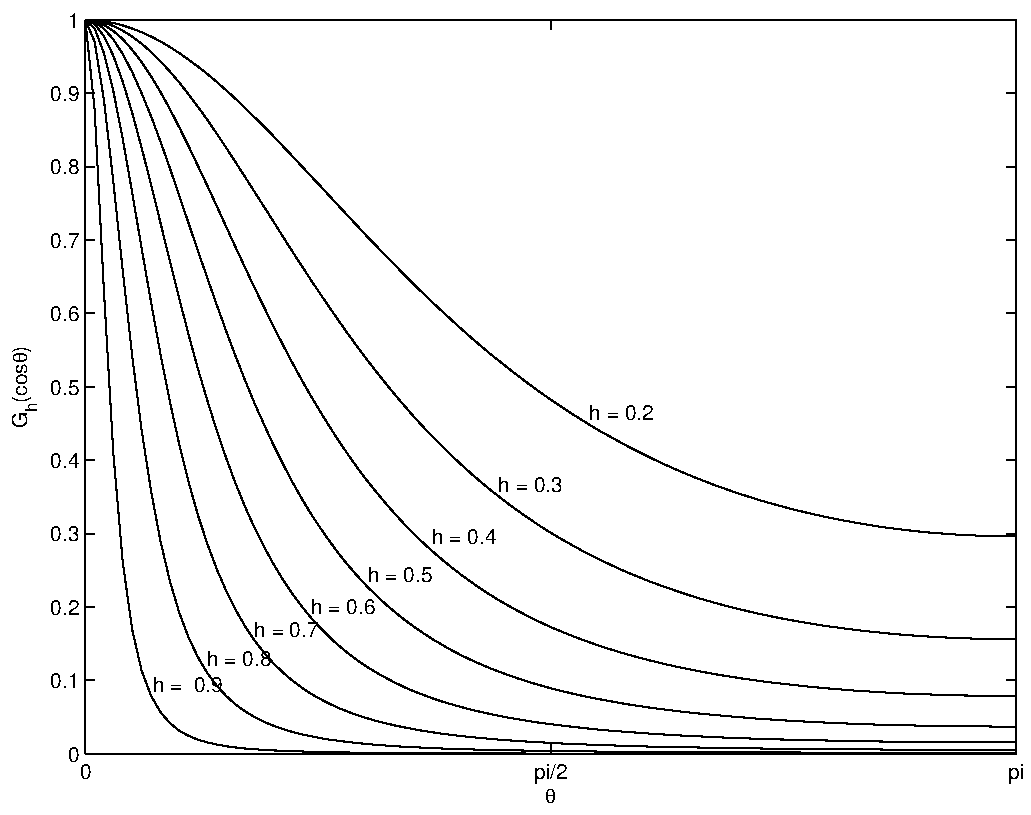
\includegraphics[height=9cm,width=12cm]{images/poisson}
  \caption{The Poisson kernel for different values of $h$. The $x$-axis is scaled
  linearly
  with respect to $\vtheta$ while the argument for the function is $t=\cos\vtheta$. Since the cosine
  function is monotone in the interval $\interv{[}{0}{\pi}{]}$, this yields a bijective mapping to
  the interval $\interv{[}{-1}{1}{]}$, where $\vtheta = 0$ and $\vtheta = \pi$ correspond to
  $t=1$ and $t=-1$. This is the fashion, this function will be used in further
  investigations. It can be seen clearly that the energy more and more concentrates around
  $\vtheta = 0$ as $h$ gets closer to 1.}
  \label{Basics.Poissonkernel}
\end{figure}


\label{Basics:SphericalKernels}

\section{Fast Polynomial Multiplication}
\label{Basics:FastPolynomialMultiplication}

\section{Nonuniform Fast Fourier Transform}
\label{Basics:NFFT}

\begin{savequote}[8cm]
  ``Suddenly, I felt like a big Nancy-boy in front of my wife. Ihad to do something to reclaim my manhood. I had to put a shelf in the closet.''
  \qauthor{Dan Zevin}
\end{savequote}
\makeatletter
\chapter{Nonequispaced Discrete Spherical Fourier Transform}
\label{DSFT}

Let in this chapter $M \in \NZ$ be fixed, $N := 2^t$ be the 
next greater power of two with respect to $M$, i.e. $t := {\ceil{\log_2 M}}$, and $\mathcal{X} := \paren{\vtheta_d,\vphi_d}_{d=0}^{D-1}$ for $D \in \N$ be
a set of nodes on $\twosphere$ called the \emph{sampling set}. As a special case, a \emph{spherical grid} 
$\mathcal{X}$ is defined by a Cartesian product 
$$
  \mathcal{X} := \pset{\vtheta_{l}}{|}{l=0,\ldots,L-1} \times \pset{\vphi_{j}}{|}{j=0,\ldots,J-1} \quad \paren{J,L \in \N}
$$
with colatitudes $\vtheta_{l} \in \interv{[}{0}{\pi}{]}$ and longitudes $\vphi_{j} \in \interv{[}{0}{2\pi}{)}$.

Given a function $f: \twosphere \rightarrow \C$, $f \in \fun{\Pol_{M}}{\twosphere}$ with Fourier expansion
\begin{equation}
  \label{NFSFT:FourierExpansion} 
  f = \sum_{\paren{k,n} \in\mathcal{I}^M} \fun{a_k^n}{f} Y_{k}^n = \sum_{k=0}^M \sum_{n=-k}^k \fun{a_k^n}{f} Y_{k}^n = \sum_{n=-M}^M \sum_{k=\abs{n}}^M \fun{a_k^n}{f} Y_{k}^n,
\end{equation}  
where 
$$\mathcal{I}^M := \pset{\paren{k,n}}{|}{k=0,\ldots,M;n=-k,\ldots,k},$$
the \emph{nonequispaced discrete spherical Fourier transform (NDSFT)} maps the coefficients $\paren{\fun{a_k^n}{f}}_{(k,n) \in \mathcal{I}^M}$ to the function values $\fun{f}{\mathcal{X}}$ on the sampling set $\mathcal{X}$.
We call $M$ the \emph{bandwidth} of $f$ and $a_{k}^n = \fun{a_{k}^n}{f}$ are the \emph{spherical Fourier coefficients} of $f$ with respect to the 
orthonormal basis of spherical harmonics $\set{Y_{k}^n}_{\paren{k,n} \in\mathcal{I}^M}$ of $\fun{\Pol_{M}}{\twosphere}$. The index $k$ will always denote the degree and $n$ always the order of $Y_{k}^n$. The Fourier coeffcients $a_{k}^n$ may be ordered 
in different ways: We refer to the \emph{degree-major order} when the Fourier coefficents are sorted first by degree $k$ and then by order $n$ in ascending order, hence
$$ a_{0}^0,\: a_{1}^{-1},\: a_{1}^{0},\: a_{1}^{1},\: a_{2}^{-2},\: \ldots,\: a_{M}^{M-1},\: a_{M}^{M}.$$ 
Analogously, the \emph{order-major order} corresponds to reversed precedence, i.e.
$$ a_{M}^{-M},\: a_{M-1}^{-(M-1)},\: a_{M}^{-(M-1)},\: a_{M-2}^{-(M-2)},\: \ldots,\: a_{M-1}^{M-1},\: a_{M}^{M-1},\: a_{M}^{M}.$$ 
From a linear algebra point of view, evaluating $f$ on $\mathcal{X}$ corresponds to a matrix-vector product
$$ \fun{\V{f}}{\mathcal{X}} = \fun{\V{Y}}{\mathcal{X}} \; \V{a}$$
with
\begin{equation}
  \nonumber
  \begin{split}
    \fun{\V{f}}{\mathcal{X}} & := \paren{f_d}_{d=0}^{D-1} \in \C^{D},\ f_{d} := \fun{f}{\vtheta_{d},\vphi_{d}},\\
    \fun{\V{Y}}{\mathcal{X}} & := \paren{\fun{Y_k^n}{\vtheta_d,\vphi_d}}_{d=0,\ldots,D-1; \paren{k,n} \in \mathcal{I}^M} \in \C^{D \times \paren{M+1}^2},\\
    \V{a} & := \paren{a_k^n}_{\paren{k,n} \in \mathcal{I}^M} \in \C^{\paren{M+1}^2}.
  \end{split}
\end{equation}
If not specified otherwise, $\V{a}$ contains the Fourier coeffcients $a_{k}^n$ in degree-mayor order and the columns of $\fun{\V{Y}}{\mathcal{X}}$ 
are ordered accordingly. 
%We drop the indices $\mathcal{X}$ and $M$ where appropriate, i.e. where they could be chosen arbitrarily or are obvious from the 
%context and write $\V{f} = \V{Y} \; \V{a}$ instead. 
Furthermore, we introduce the denotation
\begin{align*}
    \V{a}_{k} & := \paren{a_{k}^{n}}_{n=-k,\ldots,k} \in \C^{2k+1} & \paren{k=0,\ldots,M},\\
    \V{a}^{n} & := \paren{a_{k}^{n}}_{k=\abs{n},\ldots,M} \in \C^{M-\abs{n}+1} & \paren{n=-M,\ldots,M}
\end{align*} 
for subvectors of $\V{a}$. If $\mathcal{X}$ is a spherical grid, the standard order is first by colatitude $\vtheta_{l}$ and then by longitude $\vphi_{j}$. 
We use double subscripts $l,j$ to denote $\V{f}_{l,j} := \fun{f}{\vtheta_{l},\vphi_{j}}$.

A first "naive" approach to evaluating $f$ on $\mathcal{X}$ according to \eqref{NFSFT:FourierExpansion} would be to compute first all $D\:(M+1)^2$
entries of $\V{Y}$ and then perform the matrix-vector multiplication $\fun{\V{Y}}{\mathcal{X}} \: \V{a}$ the standard way. This would lead to an $\bigo{M^3 \: D}$
algorithm, since the evaluation of a function $Y_{k}^n$ at a single node already requires $\bigo{M}$ \emph{floating-point operations (flops)}.
But one can do better. Algorithm \ref{NFSFT:directDSFT} referred to as \emph{direct NDSFT} computes 
for every $\paren{\vtheta_{d},\vphi_{d}} \in \mathcal{X}$ first the sums 
\begin{equation}
  \label{NFSFT:directDSFT:firstSum}
  b^{n}_{d} := \sum_{k=\abs{n}}^M a_{k}^n \fun{P_{k}^{\abs{n}}}{\cos\vtheta_{d}} \quad \paren{n=-M,\ldots,M}. 
\end{equation}
Here one can employ the \emph{Clenshaw algorithm} (see for example \cite{prtevefl} and Algorithm \ref{NFSFT:Algorithm:Clenshaw}) the three-term recurrence 
for the associated Legendre functions from \eqref{Basics:AssociatedLegendreDefinition}. We finally compute
\begin{equation}
  \label{NFSFT:directNDSFT:secondSum}
  \fun{f}{\vtheta_{d},\vphi_{d}} = \sum_{n=-M}^M b^{n}_d \e^{\im n \vphi_{d}}
\end{equation}
directly.
\begin{algorithm}[htb]
  \caption{Clenshaw Algorithm for \eqref{NFSFT:directDSFT:firstSum}}
  \label{NFSFT:Algorithm:Clenshaw}    
  \begin{algorithmic}
    \STATE  Input: $M \in \NZ$, $n \in \Z$ with $\abs{n} \le M$, $\V{a}^n$, $x := \cos\vtheta_{d} \in \interv{[}{-1}{1}{]}$
    \STATE
    \FOR {$k=M,\ldots,\abs{n}+2$} 
      \STATE $a_{k-1}^n := a_{k-1}^n + \paren{\alpha_{k}^{|n|} x + \beta_{k}^{|n|}} a_{k}^n$
      \STATE $a_{k-2}^n := a_{k-2}^n + \gamma_{k}^{|n|} a_{k}^n$
    \ENDFOR
    \STATE $a_{\abs{n}}^n := a_{\abs{n}}^n + \paren{\alpha_{\abs{n}+1}^{|n|} x + \beta_{\abs{n}+1}^{|n|}} a_{\abs{n}+1}^n$\\[1ex]
    \STATE $b_{d}^n := \frac{((2|n|)!)}{2^{|n|} |n|!}^{1/2} \paren{1-x^2}^{|n|/2} a_{\abs{n}}^n$
    \STATE
    \STATE Output: $b_{d}^n$
\end{algorithmic}
\end{algorithm}
\begin{algorithm}[htb]
  \caption{Direct DSFT}
  \label{NFSFT:directDSFT}    
  \begin{algorithmic}
    \STATE  Input: $M \in \NZ$, $D \in \N$, $\V{a}$, $\mathcal{X}$ %$\paren{a_{k}^n}_{\paren{k,n} \in I^M}$
    \STATE
    \FOR {$d=0,\ldots,D-1$} 
      \STATE $f_{d} := 0$
      \FOR {$n=-M,\ldots,M$} 
        \STATE Compute $b^{n}_d$ by Algorithm \ref{NFSFT:Algorithm:Clenshaw} (Clenshaw algorithm),
        \STATE $f_{d} := f_{d} + b^n_d \e^{\im n \vphi_{d}}$
      \ENDFOR
    \ENDFOR
    \STATE
    \STATE Output: $\fun{\V{f}}{\mathcal{X}}$
\end{algorithmic}
\end{algorithm}
Each application of the Clenshaw algorithm for \eqref{NFSFT:directDSFT:firstSum} needs $\bigo{M}$ 
flops summing up to $\bigo{M^2}$ flops for the complete inner loop. In 
total we have an $\bigo{M^2\:D}$ algorithm for the evaluation of $f$ on $\mathcal{X}$ and gained an order of complexity with respect to $M$. 
For special sampling sets one can exploit the grid 
structure and employ FFT techniques for the sums \eqref{NFSFT:directNDSFT:secondSum} if the nodes $$\varphi_{d}$$ are equispaced 
(see \cite{drhe}, \cite{postta97} and \cite{kupo02}). 

%\citelist{\cite{Mo99} \cite{postta97} \cite{roty} \cite{suta}}

\section{Computing Fourier Coeffcients from Function Samples}
A \emph{discrete Fourier transform (DFT)} on the torus $\mathbb{T} := \pset{x \in \R}{|}{0 \le x < 2\pi}$ of length $M \in \NZ$ can be represented 
as a maxtrix-vector product
$$
  \V{f} = \V{F} \: \V{\hat{f}}
$$
with
$$
 \V{F} := \paren{\e^{2 \pi i j \frac{k}{M}}}_{j,k = 0}^{M-1} \in \C^{M \times M},\ \V{\hat{f}},\:\V{f} \in \C^{M},
$$
as well. The Fourier matrix $\V{F}$ is unitary yielding the inversion formula
\begin{equation}
  \label{NFSFT:DFTInversion}
  \V{\hat{f}} = \V{F}^{\h} \: \V{f}
\end{equation}
immediately. The DFT evaluates a trigonometric polynomial 
$$
  f := \sum_{k=0}^{M-1} \fun{\hat{f}}{k} \e^{2 \pi \im k x}
$$
at equidistant nodes $\paren{x_{d}}_{d=0}^{M-1}$ with $x_{d} := \frac{d}{M} \in \mathbb{T}$. 
For an arbitrary sampling set $\mathcal{Y}$ the associated Fourier matrix $\fun{\V{F}}{\mathcal{Y}}$ is in general no longer unitary. 
Depending on the number of Fourier coefficients and the number of nodes,
$\fun{\V{F}}{\mathcal{Y}}$ is moreover no longer square.

Having defined the NDSFT as the evaluation of a bandlimited function $f$ on a sampling set $\mathcal{X}$ on $\twosphere$, arises the question 
whether there exist sets $\mathcal{X}$ allowing for an inversion formula similar to \eqref{NFSFT:DFTInversion}.
The answer is affirmative but in general the number of nodes needed exceeds the number of Fourier coefficients to be computed, 
i.e. $\fun{\V{Y}}{\mathcal{X}}$ is not square.

We want to recover the Fourier coefficients $a_{k^n}$ from samples $\fun{\V{f}}{\mathcal{X}}$ at certain nodes $\mathcal{X}$. They 
are given by the scalar products
$$
  a_{k}^n = \scalarproduct{f}{Y_{k}^n}_{\twosphere} = \int_{0}^{2\pi} \int_{0}^{\pi} \fun{f}{\vtheta,\vphi} \overline{\fun{Y_{k}^n}{\vtheta,\vphi}} \sin \vtheta \; \dx \vtheta \; \dx \vphi \quad \paren{\paren{k,n} \in \mathcal{I}^M}.
$$
By seperating the integrand with respect to the integration variables, we obtain
\begin{eqnarray*}
  a_{k}^n & = & \int_{0}^{2\pi} \int_{0}^{\pi} \fun{f}{\vtheta,\vphi} \fun{P_{k}^{\abs{n}}}{\cos \vtheta} \e^{-\im n \vphi} \sin \vtheta \; \dx \vtheta \; \dx \vphi\\
          & = & \int_{0}^{\pi} \fun{P_{k}^{\abs{n}}}{\cos \vtheta} \sin \vtheta \; \int_{0}^{2\pi} \fun{f}{\vtheta,\vphi} \e^{-\im n \vphi} \; \dx \vphi \; \dx \vtheta.
\end{eqnarray*}
For the integrals
$$
  \fun{f_{n}}{\vtheta} := \int_{0}^{2\pi} \fun{f}{\vtheta,\vphi} \e^{-\im n \vphi} \; \dx \vphi
$$
we have the quadrature rule
$$ \fun{f_{n}}{\vtheta} = \frac{1}{2(M+1)} \sum_{j=0}^{2M+1} \fun{f}{\vtheta,\vphi_{j}} \e^{-\im n \vphi_{j}}$$
where
$$ \vphi_{j} := \frac{j\pi}{N} \quad \paren{j=0,\ldots,2M+1}. $$
This holds due to the Sampling Theorem by taking into account that for fixed $\vtheta$ the function
\begin{eqnarray*}
  \fun{f}{\vtheta,\vphi} & = & \sum_{n=-M}^{M} \left(\sum_{k=\abs{n}}^M a_{k}^n \fun{P_{k}^{\abs{n}}}{\cos \vtheta}\right) \e^{-\im n \vphi}\\
\end{eqnarray*}
is a trigonometric polynomial of degree $M$ in $\vphi$ with Fourier coefficients
$$
  c_{n} := \sum_{k=\abs{n}}^M a_{k}^n \fun{P_{k}^{\abs{n}}}{\cos \vtheta}.
$$
It remains to compute
$$
  a_{k}^n = \int_{0}^{\pi} \fun{P_{k}^{\abs{n}}}{\cos \vtheta} \fun{f_{n}}{\vtheta} \sin \vtheta \; \dx \vtheta = 
  \int_{-1}^1 \fun{P_{k}^{\abs{n}}}{x} \fun{f_{n}}{\arccos x} \; \dx x.
$$
By verifying that $\fun{P_{k}^{\abs{n}}}{x} \fun{f_{n}}{\arccos x}$ is an algebraic polynomial of degree at most $2M+1$, 
we can use various types of quadrature rules. We first mention the \emph{Gauss-Legendre} quadrature rule
$$
  \int_{0}^{\pi} \fun{P_{k}^{\abs{n}}}{\cos \vtheta} \fun{f_{n}}{\vtheta} \sin \vtheta \; \dx \vtheta = \sum_{l=0}^{M} w_{l}^{\gl} \fun{P_{k}^{\abs{n}}}{\cos \vtheta_{l}^{\gl}} \fun{f_{n}}{\vtheta_{l}} 
$$
with nodes $\paren{\vtheta_{l}^{\gl}}_{l=0}^M$ and weights $\paren{w_{l}^{\gl}}_{l=0}^M$ as described for example in \cite{boehme02}. 
We notice that the $M+1$ nodes $\paren{\vtheta_{l}^{\gl}}_{l=0}^{M}$ can be computed as the eigenvalues of the \emph{Jacobi matrix} for the orthogonal 
Legendre polynomials. The weights $\paren{w_{l}}_{l=0}^{M}$ are obtained from the corresponding eigenvectors.

A second idea is to employ a Clenshaw-Curtis quadrature rule (see \cite{dara}, pp. 86)
$$
  \int_{0}^{\pi} \fun{P_{k}^{\abs{n}}}{\cos \vtheta} \fun{f_{n}}{\vtheta} \sin \vtheta \; \dx \vtheta = \sum_{l=0}^{2M} \varepsilon_{l}^{2M} w_{l}^{\cc} \fun{P_{k}^{\abs{n}}}{\cos \vtheta_{l}^{\cc}} \fun{f_{n}}{\vtheta_{l}}
$$
where $\varepsilon_{0}^{M} := \epsilon_{M}^M := \frac{1}{2}$, $\epsilon_{l}^M := 1$, $l=1,\dots,M-1$, and $\vtheta_{l}^{\cc} = \frac{l\pi}{2M}$ are the \emph{Chebyshev nodes}.
This quadrature rule uses almost twice as many points as the Gauss-Legendre quadrature rule but allows for an easy and fast online computation of the nodes $\vtheta_{l}^{\cc}$
and weights $w_{l}^{\gl}$. The weights are given by
$$ w_{l}^{\gl} := \frac{1}{2M} \sum_{j=0}^{M} \varepsilon_{j}^{M} \frac{-2}{4j^2-1} \cos\frac{lj\pi}{M}.$$
This finally yields for the Fourier coeffcients $a_{k}^n$ the identities 
\begin{equation}
  \label{NFSFT:iDSFT}
  \begin{split}
    a_{k}^n & = \frac{1}{2(M+1)} \sum_{j=0}^{2(M+1)-1} \sum_{l=0}^{M} w_{l}^{\gl} \fun{f}{\vtheta_{l}^{\gl},\vphi_{j}} \overline{\fun{Y_{k}^n}{\vtheta_{l}^{\gl},\vphi_{j}}},\\
    a_{k}^n & = \frac{1}{2(M+1)} \sum_{j=0}^{2(M+1)-1} \sum_{l=0}^{2M} \varepsilon_{l}^{2M} w_{l}^{\cc} \fun{f}{\vtheta_{l}^{\cc},\vphi_{j}} 
  \overline{\fun{Y_{k}^n}{\vtheta_{l}^{\cc},\vphi_{j}}}.
  \end{split}
\end{equation}
Associated with this quadrature formulae, we define the sampling sets
\begin{eqnarray*}
  \mathcal{X}^{\gl} & := & \paren{\vtheta_{l}^{\gl},\vphi_{j}}_{j=0,\dots,2(M+1)-1;l=0,\dots,M},\\
  \mathcal{X}^{\cc} & := & \paren{\vtheta_{l}^{\cc},\vphi_{j}}_{j=0,\dots,2(M+1)-1;l=0,\dots,2M}
\end{eqnarray*}
and refer to $\mathcal{X}^{\gl}$ as the \emph{Gauss-Legendre sampling set of degree M} and to $\mathcal{X}^{\cc}$ as the 
\emph{Clenshaw-Curtis sampling set of degree M}. These two types of sampling sets are illustrated in Figure \ref{quadrature}.
\begin{figure}[tb]
  \centering
  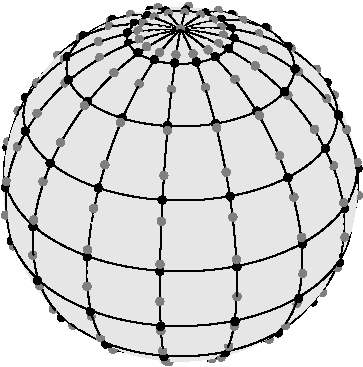
\includegraphics[width=12cm]{images/quadrature}
  \caption{The sample sets $\mathcal{X}^{\gl}$ (red dots) and $\mathcal{X}^{\cc}$ (green dots) for $M=7$.}
  \label{quadrature}
\end{figure}
We now immediately obtain the corresponding inversion formulae
\begin{equation}
  \label{NFSFT:InversionFormula}
  \begin{split}
    \V{a} & = \fun{\V{Y}}{\mathcal{X}^{\gl}}^{\h} \: \V{W}^{\gl} \: \fun{\V{f}}{\mathcal{X}^{\gl}},\quad \V{W}^{\gl} := \V{I}_{2M+2} \otimes \diag\paren{w_{l}^{\gl}}_{l=0}^M,\\
    %\label{NFSFT:InversionFormulaCC}
    \V{a} & = \fun{\V{Y}}{\mathcal{X}^{\cc}}^{\h} \: \V{W}^{\cc} \: \fun{\V{f}}{\mathcal{X}^{\cc}},\quad \V{W}^{\cc} := \V{I}_{2M+2} \otimes \diag\paren{\varepsilon_{l}^{2M}w_{l}^{\cc}}_{l=0}^M.
  \end{split}  
\end{equation}  
An algorithm for the multiplication with the adjoint matrix $\V{Y}^{\h}$ is the key for an implementation according to \eqref{NFSFT:InversionFormula}. Evaluating the matrix-vector product the standard way, i.e. row-wise for $\V{Y}^{\h}$, a first approach would be to compute the Fourier coefficients $a_{k}^n$ by \eqref{NFSFT:iDSFT} for all $\paren{k,n} \in \mathcal{I}^M$ employing the Clenshaw algorithm for the evaluation of the functions $Y_{k}^n$. But this would again lead to an $\bigo{M^3 \: D}$ algorithm. This is due to the fact, that the Clenshaw algorithm would now be applied to each function $Y_{k}^n$ seperately instead of evaluating a linear combination for fixed $n$ and $k = \abs{n},\dots,M$ as in Algorithm \ref{NFSFT:directDSFT}. If we recall that we would end up with a $\bigo{M^3 \: D}$ algorithm for the NDSFT, too, if we evaluated the matrix $\V{Y}$ componentwise and then performed the matrix-vector multiplication as usual, we notice that Algorithm \ref{NFSFT:directDSFT} implies a factorization of $\V{Y}$ into a product of sparse matrices therefore allowing us to save one order of $M$. Furthermore, by taking the adjoint factorization, we obtain a corresponding factorization of $\V{Y}^{\h}$ immediately. This allows for the derivation of an algorithm of exactly the same asymptotic complexity for computing the adjoint product, too.

\section{A Factorization of the Fourier Matrix}

In order to abtain an $\bigo{M^2 \: D}$ algorithm for the adjoint product, we first derive the factorization of $\V{Y}$ according to Algorithm \ref{NFSFT:directDSFT}. The matrix $\V{Y}$ can be written as
$$
  \V{Y} = 
    \left[\begin{array}{c}
      \V{E}_{0}\\
      \V{E}_{1}\\
      \vdots\\
      \V{E}_{D-1}
    \end{array}\right], \quad \V{E}_{d} \in \C^{1 \times (M+1)^2} \quad \paren{d=0,\ldots,D-1}.
$$
Each matrix $\V{E}_{d}$ evaluates $f$ at $\paren{\vtheta_{d},\vphi_{d}}$ according to 
$$
  \fun{f}{\vtheta_{d},\vphi_{d}} = \sum_{n=-M}^M \sum_{k=\abs{n}}^M a_k^n \fun{Y_{k}^n}{\vtheta_{d},\vphi_{d}}.
$$
So let $d$ be fixed. The algorithms begins by evaluating the sums
$$
  b^{n}_{d} = \sum_{k=\abs{n}}^M a_{k}^n \fun{P_{k}^{\abs{n}}}{\cos\vtheta_{d}} \quad \paren{n=-M,\ldots,M}. 
$$
which corresponds to computing
$$
  \left(\begin{array}{c}
    b^{-M}_{d}\\
    b^{-(M-1)}_{d}\\
    \vdots\\
    b^{M}_{d}
  \end{array}\right)
  =
  \left[\begin{array}{cccc}
    \V{C}^{-M}_{d} &                    &        &               \\
                   & \V{C}^{-(M-1)}_{d} &        &               \\
                   &                    & \ddots &               \\
                   &                    &        & \V{C}^{M}_{d} 
  \end{array}\right]
  \:
  \left[\begin{array}{c}
    \V{a}^{-M}\\
    \V{a}^{-(M-1)}\\
    \vdots\\
    \V{a}^{M}
  \end{array}\right]
$$
where each matrix $\V{C}^{n}_{d} \in \R^{1 \times (M-n+1)}$ for $n = -M,\ldots,M$ realizes the Clenshaw algorithm \ref{NFSFT:Algorithm:Clenshaw} acting on the subvector $\V{a}^n$ of $\V{a}$.
They can be further decomposed corresponding to the number of steps in the Clenshaw algorithm by
\begin{eqnarray*}
  \V{C}^{n}_{d}       & := & \frac{((2|n|)!)}{2^{|n|} |n|!}^{1/2} \paren{1-\cos^2\vtheta_{d}}^{|n|/2} \V{C}_{d,1}^{n} \: \V{C}_{d,2}^{n} \: \ldots \: \V{C}_{d,M-\abs{n}}^{n},\\
  \V{C}_{d,l}^{n}     & := & \encl{[}{\V{I}_{l}, \V{\tilde{e}}_{d,l}}{]} \in \R^{l \times (l+1)},\\
  \V{\tilde{e}}_{d,l} & := & \paren{0,0,\ldots,\gamma_{k}^n,\alpha_{k}^n \vtheta_{d} + \beta_{k}^n}^{\transp} \in \R^{l} \quad \paren{l=1,\ldots,M-\abs{n}}.
\end{eqnarray*}
Finally, we compute the sum
$$
  f_{d} = \sum_{n=-M}^M b^{n}_{d} \e^{\im n \vphi_{d}}
$$
by the scalar product
$$
  f_{d} 
  = 
%  \V{E}_{d}
%  \:
%  \V{a}
%  =
  \paren{\e^{\im (-M) \vphi_{d}},\e^{\im (-(M-1)) \vphi_{d}},\ldots,\e^{\im M \vphi_{d}}}
  \:   
  \left(\begin{array}{c}
    b^{-M}_{d}\\
    b^{-(M-1)}_{d}\\
    \vdots\\
    b^{M}_{d}
  \end{array}\right).
$$
This gives the representation
$$
  \V{E}_{d} = \paren{\e^{\im (-M) \vphi_{d}},\e^{\im (-(M-1)) \vphi_{d}},\ldots,\e^{\im M \vphi_{d}}} \:  
  \left[\begin{array}{cccc}
    \V{C}^{-M}_{d} &                    &        &               \\
                   & \V{C}^{-(M-1)}_{d} &        &               \\
                   &                    & \ddots &               \\
                   &                    &        & \V{C}^{M}_{d} 
  \end{array}\right].
$$

\section{Adjoint and Inverse DSFT}

We obtain the sought algorithm for the adjoint transform directly from the factorization given in the last section. We have to evaluate
$$
  \V{\tilde{a}}
  :=
  \V{Y}^{\h} \V{f}
  = 
  \encl{[}{
    \V{E}_{0}^{\h},
    \V{E}_{1}^{\h},
    \ldots,
    \V{E}_{D-1}^{\h}
  }{]}
  \:
  \left(\begin{array}{c}
    f_{0}\\
    f_{1}\\
    \vdots\\
    f_{D-1}
  \end{array}\right). 
$$
This decomposition implies the evaluation of the matrix-vector product in a nonstandard way by traversing the 
matrix column-wise instead of row-wise. After each column $\V{E}_{d}^{\h}$, the result vector is updated with the portion due 
to the product $\V{\tilde{a}}_{d} := \V{E}^{\h}_{d} \: f_{d}$. We obtain
\begin{equation}
  \nonumber
  \V{\tilde{a}} = \V{\tilde{a}}_{0} + \V{\tilde{a}}_{1} + \ldots + \V{\tilde{a}}_{D-1}
\end{equation}
and
\begin{equation}
  \label{NFSFT:adjointNDSFTFactorization}
  \V{\tilde{a}}_{d}
  =
  \left[\begin{array}{cccc}
    {\V{C}^{-M}_{d}}^{\transp} &                               &        &                           \\
                              & {\V{C}^{-(M-1)}_{d}}^{\transp} &        &                           \\
                              &                                & \ddots &                           \\
                              &                                &        & {\V{C}^{M}_{d}}^{\transp} 
  \end{array}\right]
  \:
  \left(\begin{array}{c}
    \e^{\im M \vphi_{d}}\\
    \e^{\im (M-1) \vphi_{d}}\\
    \vdots\\
    \e^{\im (-M) \vphi_{d}}
  \end{array}\right)
  \:
  f_{d}.
\end{equation}
A multiplication with a transposed matrix ${\V{C}^{n}_{d}}^{\transp}$ realizes a \emph{"transposed" Clenshaw algorithm} summarized in Algorithm \ref{NFSFT:transposedClenshaw}. The complete algorithm can be obtained from \eqref{NFSFT:adjointNDSFTFactorization} directly and is given in Algorithm \ref{NFSFT:adjointDSFT}.
\begin{algorithm}[htb]
  \caption{Transposed Clenshaw Algorithm}
  \label{NFSFT:transposedClenshaw}    
  \begin{algorithmic}
    \STATE  Input: $M \in \NZ$, $n \in \NZ$ with $\abs{n} \le M$, $\tilde{b}^n_{d}$, $x := \cos\vtheta_{d} \in \interv{[}{-1}{1}{]}$
    \STATE
    \STATE $\tilde{a}_{d,\abs{n}-1}^n := 0$
    \STATE $\tilde{a}_{d,\abs{n}}^n := \frac{((2|n|)!)}{2^{|n|} |n|!}^{1/2} \paren{1-x^2}^{|n|/2} \tilde{b}^n_{d}$
    \FOR {$k=\abs{n}+1,\ldots,M$} 
      \STATE $\tilde{a}_{d,k}^n := \paren{\alpha_{k}^n\vtheta_{d} + \beta_{k}^n}\tilde{a}_{d,k-1}^n + \gamma_{k}^n \tilde{a}_{d,k-2}^n$
    \ENDFOR
    \STATE
    \STATE Output: $\V{\tilde{a}}^n_{d}$
\end{algorithmic}
\end{algorithm}
\begin{algorithm}[htb]
  \caption{Adjoint DSFT}
  \label{NFSFT:adjointDSFT}    
  \begin{algorithmic}
    \STATE  Input: $M \in \NZ$, $D \in \N$, $\mathcal{X}$, $\fun{\V{f}}{\mathcal{X}}$
    \STATE
    \FOR {$n=-M,\ldots,M$} 
      \FOR {$k=\abs{n},\ldots,M$} 
        \STATE $\tilde{a}_{k}^n := 0;$
      \ENDFOR
    \ENDFOR
    \FOR {$d=0,\ldots,D-1$} 
      \FOR {$n=-M,\ldots,M$} 
        \STATE $\tilde{b}^n_{d} := f_{d} \: \e^{\im n \vphi_{d}}$
        \STATE Compute $\V{\tilde{a}}^n_{d}$ by the transposed Clenshaw algorithm
        \STATE $\V{\tilde{a}}^n := \V{\tilde{a}}^n + \V{\tilde{a}}^n_{d}$
      \ENDFOR
    \ENDFOR
    \STATE
    \STATE Output: $\V{\tilde{a}}$
\end{algorithmic}
\end{algorithm}

We have now obtained an $\bigo{M^2\:D}$ algorithm for the multiplication with $\V{Y}^{\h}$. Based on \ref{NFSFT:InversionFormula} and algorithm \ref{NFSFT:adjointDSFT} we obtain $\bigo{M^4}$ algorithms \ref{NFSFT:directIDSFTGL} and \ref{NFSFT:directIDSFTCC} for computing the Fourier coeffcients $a_{k}^n$ from the function samples $\fun{\V{f}}{\mathcal{X}^{\gl}}$ and $\fun{\V{f}}{\mathcal{X}^{\cc}}$. We refer to these algorithms as the \emph{direct inverse discrete spherical Fourier transform} of \emph{Gauss-Legendre type (iDSFT-GL)} and \emph{Clenshaw-Curtis type (iDSFT-CC)}, respectively.

\begin{algorithm}[htb]
  \caption{Direct iDSFT-GL}
  \label{NFSFT:directIDSFTGL}    
  \begin{algorithmic}
    \STATE Input: $M \in \NZ$, $\fun{\V{f}}{\mathcal{X}^{\gl}}$
    \STATE
    \FOR {$j = 0,\ldots,2M+1$}
      \FOR {$l = 0,\ldots,M$}
        \STATE $f_{j,l} = w^{\gl}_{l} f_{j,l}$ 
      \ENDFOR
    \ENDFOR
    \STATE Compute $\V{a}$ by an adjoint DSFT
    \STATE
    \STATE Output: $\V{a}$
  \end{algorithmic}
\end{algorithm}
\begin{algorithm}[htb]
  \caption{Direct iDSFT-CC}
  \label{NFSFT:directIDSFTCC}    
  \begin{algorithmic}
    \STATE Input: $M \in \NZ$, $\fun{\V{f}}{\mathcal{X}^{\cc}}$
    \STATE
    \FOR {$j = 0,\ldots,2M+1$}
      \FOR {$l = 0,\ldots,2M$}
        \STATE $f_{j,l} = \varepsilon_{l}^{2M} w^{\cc}_{l} f_{j,l}$ 
      \ENDFOR
    \ENDFOR
    \STATE Compute $\V{a}$ by an adjoint DSFT
    \STATE
    \STATE Output: $\V{a}$
  \end{algorithmic}
\end{algorithm}

The algorithms for the computation of the products $\fun{\V{f}}{\mathcal{X}} = \fun{\V{Y}}{\mathcal{X}} \: \V{a}$ and $\V{\tilde{a}} = \fun{\V{Y}}{\mathcal{X}}^{\h} \: \fun{\V{f}}{\mathcal{X}}$ presented so far have both computational complexity $\bigo{M^2\:D}$ making computations for most applications impracticably slow. We already mentioned that FFT techniques may be applied to sums of the form
$$
  f_{d} := \sum_{n = -M}^M b^n_d \e^{\im n \vphi_{d}} \quad \paren{d = 0,\ldots,D}
$$
if the nodes $\vphi_d$ are distributed uniformly. For a nonuniform distribution one may apply the NFFT algorithm from Section \ref{Basics:NFFT}. In the following section we present a fast algorithm for the evaluation of the sums $b^{n}_{d}$ from \eqref{NFSFT:directDSFT:firstSum} first mentioned in \cite{postta97}. To be more precise, the algorithm performs for a fixed $n$ a change of basis independent of the nodes to transform a sum of the form
\begin{equation}
  \label{NFSFT:LegendreSum}
  \sum_{k=\abs{n}}^M a_{k}^n \fun{P_{k}^n}{x}
\end{equation}
into a representation by Chebyshev polynomials. This is possible since the associated Legendre functions $P_{k}^n$ are (up to a factor $\frac{1}{\sqrt{1-x^2}}$ for odd $n$) polynomials of degree at most $M$. Once obtained this representation and taking into account that the argument $x$ takes the form $\cos \vtheta$, one may rewrite the sum again as an ordinary Fourier sum that can be evaluated by the NFFT algorithm at nonequispaced nodes in a fast way, too. In total this results in an approximative $\bigo{M^2 \log^2 M + mD}$ algorithm, where $m$ is a constant depending on the desired accuracy. 

%This holds only in the case of equispaced nodes. If one leaves 
%In this chapter, we first derive an algorithm for the fast evaluation of a bandlimited function $f$ at arbitrary nodes. Due to the separability 
%of the basis functions $Y_k^n$, evaluating the sum in \eqref{NFSFT:FourierExpansion} can be split up in ordinary discrete Fourier transforms for nonequispaced 
%data in colatitudinal direction and \emph{discrete Legendre function transforms} for the latitudinal part. The basic idea of the approach 
%presented here is to perform a change of basis from Legendre functions to complex exponentials in latitudinal direction to get the 
%representation
%$$ \fun{f}{\vtheta,\vphi} = \sum_{n=-M}^{M} \sum_{k=-M}^M c_k^n e^{ik\vtheta} e^{in\vphi}.$$
%The computation of the function values $f_j := \fun{f}{\vtheta_j,\vphi_j}$ can now be performed 
%using a two-dimensional NFFT. 

%Once derived a fast algorithm for this product, which implies a factorization of $\V{Y}$ into a product of sparse matrices,
%one also immediately gets from the theoretical point of view a fast algorithm for the adjoint product 
%$$\V{a} = \V{Y}^{\h} \; \V{f}.$$

\section{Fast Legendre Function Transform}
\label{DSFT:FLFT}

In this and the following section, we assume $n \ge 0$ without loss of generality. We consider polynomials of the form
\begin{equation}
  \label{NFSFT:GnEven}
 \fun{g^n}{x} := \sum_{k=n}^M a_k^n \fun{P_k^n}{x} \in \Pol_M
 \end{equation}
for even $n$ and
\begin{equation}
  \label{NFSFT:GnOdd}
  \fun{g^n}{x} := \frac{1}{\sqrt{1-x^2}} \sum_{k=n}^M a_k^n \fun{P_k^n}{x} \in \Pol_{M-1}
\end{equation}
for odd $n$ with given complex coefficients $a_k^n$.
The \emph{fast Legendre tunction transform (FLFT)} performes a change of basis and computes the 
coefficients $b_k^n$ of the Chebyshev representation
$$ \fun{g^n}{x} = \sum_{k=0}^M b_k^n \fun{T_k}{x}$$
for even $n$ and
$$\fun{g^n}{x} = \sum_{k=0}^{M-1} b_k^n \fun{T_k}{x}$$
for odd $n$.

Lemma \ref{Basics:AssociatedLegendreRecurrence} implies
\begin{equation}
  \label{NFSFT:U}
  \left(\begin{array}{c}
    P_{c+k}^{n} \\ P_{c+k+1}^{n}
  \end{array}\right)
  =
  \fun{U_{k}^{n}}{\cdot,c}^{\transp}\;
  \left(\begin{array}{c}
    P_{c-1}^{n} \\ P_{c}^{n}
  \end{array}\right)
\end{equation}
where
$$
  \fun{U_{k}^{n}}{\cdot,c}^{\transp} :=
  \left(\begin{array}{cc}
    \gamma_c^{n} \fun{P_{k-1}^{n}}{\cdot,c+1} & \gamma_c^{n} \fun{P_{k}^{n}}{\cdot,c+1} \\
                 \fun{P_{k}^{n}}{\cdot,c}     &              \fun{P_{k+1}^{n}}{\cdot,c}
  \end{array}\right).   
$$
We set $a_k^n := 0$ for $k < n$ or $k > M$. In a first step, we use Lemma 
\ref{Basics:AssociatedLegendreRecurrence} to write
$$ g^n = \sum_{k = n}^{N-1} a_{k}^{(0)} P_k^{n}$$
with
\begin{eqnarray*}
  \fun{a_k^{(0)}}{x}     & := & a_k^n \quad (k = 0,\ldots,N-3),\\
  \fun{a_{N-2}^{(0)}}{x} & := & a_{N-2}^n + \gamma_{N-1}^{n} a_N^n,\\
  \fun{a_{N-1}^{(0)}}{x} & := & a_{N-1}^n + \paren{\alpha_{N-1}^{n}x + \beta_{N-1}^{n}} a_N^n.
\end{eqnarray*}
We now set 
$$\tilde{n} := \fun{\min}{n,N-2}, \quad \tilde{M} := \left\{\begin{array}{l@{\quad \text{if} \quad}l} M & M < N, \\ M-1 & M = N.\end{array}\right.$$
and obtain
$$
  g^n = \sum_{l = \floor{\frac{\tilde{n}}{4}}}^{\ceil{\frac{\tilde{M}+1}{4}}-1} \paren{\sum_{k=0}^{3} a_{4l+k}^{(0)} P_{4l+k}^{n}}.
$$

Notice that $a_k^{(0)}$ are polynomials of 
degree at most $1$ and that one immediately has their corresponding Chebyshev coefficients.

From \eqref{NFSFT:U} with $k = 1$ and $c = l+1$ it follows that
$$
\left(\begin{array}{c}
  P_{4l+2}^{n}, 
  P_{4l+3}^{n}
\end{array}\right)
\left(\begin{array}{c}
  a_{4l+2}^{(0)}\\
  a_{4l+3}^{(0)} 
\end{array}\right)
=
\left(\begin{array}{c}
  P_{4l}^{n},
  P_{4l+1}^{n}
\end{array}\right)
{\mathbf{U}_{1}^{n}\left(\cdot,4l+1\right)}
\left(\begin{array}{c}
  a_{4l+2}^{(0)}\\
  a_{4l+3}^{(0)} 
\end{array}\right)
$$
and therefore
$$ g^n = \sum_{l = \floor{\frac{\tilde{n}}{4}}}^{\ceil{\frac{\tilde{M}+1}{4}}-1} a_{4l}^{(1)} \paren{P_{4l}^{n} + a_{4l+1}^{(1)} P_{4l+1}^{n}} $$
with
\begin{equation}
\label{NFSFT:FirstStep}
  \left(\begin{array}{c}
    a_{4l}^{(1)}\\
    a_{4l+1}^{(1)} 
  \end{array}\right)
  =
  \left(\begin{array}{c}
    a_{4l}^{(0)}\\
    a_{4l+1}^{(0)} 
  \end{array}\right)
  + {\mathbf{U}_{1}^{n}\left(\cdot,4l+1\right)}
  \left(\begin{array}{c}
    a_{4l+2}^{(0)}\\
    a_{4l+3}^{(0)} 
  \end{array}\right).
\end{equation}
We can use Algorithm \ref{Basics:Algorithm:FastPolynomialMultiplication} with $K=2$ to compute 
the polynomial products in \eqref{NFSFT:FirstStep}. Applying this idea repeatedly leads to a cascade 
summation with steps $\tau=1,\ldots,t-1$ as illustrated in Figure \ref{NFSFT:Figure:CascadeSummation}. 
In step $\tau$ we compute
\begin{equation}
  \label{NFSFT:GeneralStep}
  \left(\begin{array}{c}
    a_{2^{\tau+1}l}^{(\tau)}\\
    a_{2^{\tau+1}l+1}^{(\tau)} 
  \end{array}\right)
  =
  \left(\begin{array}{c}
    a_{2^{\tau+1}l}^{(\tau-1)}\\
    a_{2^{\tau+1}l+1}^{(\tau-1)} 
  \end{array}\right)
  + {\fun{\V{U}_{2^{\tau}-1}^{n}}{\cdot,2^{\tau+1}l+1}}
  \left(\begin{array}{c}
    a_{2^{\tau+1}l+2^{\tau}}^{(\tau-1)}\\
    a_{2^{\tau+1}l+2^{\tau}+1}^{(\tau-1)} 
  \end{array}\right)
\end{equation}
for $\paren{l=\floor{\frac{\tilde{n}}{2^{\tau+1}}},\ldots,\ceil{\frac{\tilde{M}+1}{2^{\tau+1}}}-1}$
by applying Algorithm \ref{Basics:Algorithm:FastPolynomialMultiplication} with $N=2^{\tau}$. It can be shown that
$a_{2^{\tau+1}l}^{(\tau)} = a_{2^{\tau+1}l+1}^{(\tau)} \equiv 0$ for $l < \floor{\frac{\tilde{n}}{2^{\tau+1}}}$ and 
$l > \ceil{\frac{\tilde{M+1}}{2^{\tau+1}}}-1$.
After step $\tau = t-1$ we arrive at
\begin{equation}
  \nonumber
  g^n = a_{0}^{(t-1)} P_{0}^{n} + a_{1}^{(t-1)} P_{1}^{n}.
\end{equation}
Since 
\begin{equation}
  \nonumber
  \fun{P_{0}^n}{x} = \frac{\left( \left( 2n \right) ! \right)^{1/2}}{2^n n!},\ \fun{P_{1}^n}{x} = \left(\alpha_{0}^nx + \beta_{0}^n\right)\fun{P_{0}^n}{x}
\end{equation} 
we get
\begin{equation}
  \label{NFSFT:LastStep}
  g^n = \frac{\left( \left( 2n \right) ! \right)^{1/2}}{2^n n!} a_{0}^{(t-1)} + a_{1}^{(t-1)} \left(\alpha_{0}^nx + \beta_{0}^n\right)\fun{P_{0}^n}{x}
\end{equation}
Using 
\begin{equation}
  \nonumber
  xT_{0}(x) = T_{1}(x),\ xT_{k}(x) = \frac{1}{2}\left( T_{k+1}(x) + T_{k-1}(x) \right)
\end{equation}
we finally obtain the sought Chebyshev coeffcients $b_{k}^n$ of $g^n$ from \eqref{NFSFT:LastStep} by
applying elementary vector operations on the vectors of Chebyshev coefficients of $a_{0}^{(t-1)}$ and $a_{1}^{(t-1)}$ 
(see Section \ref{NFSFT:LinearAlgebra:LastStep}).

In total, the FLFT consists of $t+1 = \bigo{\log M}$ steps. The first and the last step clearly have computational complexity $\bigo{M}$. The rest of the steps is the cascade summation. Each step has computational complexity $\bigo{M \log M}$ due to the DCT applications in Algorithm \ref{Basics:Algorithm:FastPolynomialMultiplication} used for the multiplication with the matrices $U$. In total this accumulates to $\bigo{M \log^2 M}$ for the whole algorithm.

\begin{figure}
  \label{NFSFT:Figure:CascadeSummation}
  % Cascade summation
  \unitlength0.87cm
    \begin{picture}(14,14)
      % setze 6 Boxen
      \multiput(0,0)(0,2.5){6}{\framebox(14,1)[lb]}
      % schreibe in die 1. Box
      \multiput(1.64,12.5)(1.64,0){8}{\line(0,1){1}}
      %\put(14.4,12.8){\large $\in \mathbb R$}
      \put(0.3,12.8){\large $0$}
      \put(1.0,12.8){\large $0$}
      \put(1.94,12.8){\large $0$}
      \put(2.64,12.8){\large $0$}
      \put(3.59,12.8){\large $a_4^4$}
      \put(4.29,12.8){\large $a_5^4$}
      \put(5.24,12.8){\large $a_6^4$}
      \put(5.94,12.8){\large $a_7^4$}
      \put(6.88,12.8){\large $a_8^4$}
      \put(7.58,12.8){\large $a_9^4$}
      \put(8.45,12.8){\large $a_{10}^4$}
      \put(9.15,12.8){\large $a_{11}^4$}
      \put(10.1,12.8){\large $a_{12}^4$}
      \put(10.8,12.8){\large $a_{13}^4$}
      \put(11.75,12.8){\large $a_{14}^4$}
      \put(12.4,12.8){\large $a_{15}^4$}
      \put(13.3,12.8){\large $a_{16}^4$}
      % schreibe zwischen 2. und 3. Box
      \multiput(12.2,11.5)(1.3,0){2}{\line(0,1){1}}
      \put(12.2,11.5){\line(1,0){1.3}}
      \put(12.7,11){\line(0,1){0.5}}
      %\multiput(0.82,11)(1.64,0){7}{\line(0,1){1.5}}
      \multiput(4.12,11)(1.64,0){5}{\line(0,1){1.5}}
      % schreibe in die 2. Box
      \multiput(1.64,10)(1.64,0){7}{\line(0,1){1}}
      %\put(14.4,10.3){\large $\in \Pi_1$}
      \put(0.3,10.3){\large $0$}
      \put(1.0,10.3){\large $0$}
      \put(1.94,10.3){\large $0$}
      \put(2.64,10.3){\large $0$}
      \put(3.5,10.3){\large $a_4^{(0)}$}
      \put(4.2,10.3){\large $a_5^{(0)}$}
      \put(5.1,10.3){\large $a_6^{(0)}$}
      \put(5.8,10.3){\large $a_7^{(0)}$}
      \put(6.75,10.3){\large $a_8^{(0)}$}
      \put(7.45,10.3){\large $a_9^{(0)}$}
      \put(8.35,10.3){\large $a_{10}^{(0)}$}
      \put(9.05,10.3){\large $a_{11}^{(0)}$}
      \put(10.05,10.3){\large $a_{12}^{(0)}$}
      \put(10.7,10.3){\large $a_{13}^{(0)}$}
      \put(11.85,10.3){\large $a_{14}^{(0)}$}
      \put(13.00,10.3){\large $a_{15}^{(0)}$}
      % schreibe zwischen 2. und 3. Box
      %\multiput(0.82,9)(1.64,0){7}{\line(0,1){1}}
      \multiput(4.10,9)(1.64,0){5}{\line(0,1){1}}
      \put(12.8,9){\line(0,1){1}}
      %\multiput(0.82,9)(3.28,0){3}{\line(1,0){1.64}}
      \multiput(4.10,9)(3.28,0){2}{\line(1,0){1.64}}
      \put(10.66,9){\line(1,0){2.14}}
      %\multiput(1.64,8.5)(3.28,0){4}{\line(0,1){0.5}}
      \multiput(4.92,8.5)(3.28,0){3}{\line(0,1){0.5}}
      %\put(0.95,9.3){$ U_1^4(\, \cdot\, ,1)$}
      \put(4.23,9.3){$ U_1^4(\, \cdot\, ,5)$}
      \put(7.5,9.3){$ U_1^4(\, \cdot\, ,9)$}
      \put(10.9,9.3){$ U_1^4(\; \cdot\; ,13)$}
      % schreibe in die 3. Box
      \multiput(3.3,7.5)(3.3,0){3}{\line(0,1){1}}
      %\put(14.4,7.8){\large $\in \Pi_3$}
      \put(0.82,7.8){\large $0$}
      \put(2.2,7.8){\large $0$}
      \put(3.8,7.8){\large $a_4^{(1)}$}
      \put(5.5,7.8){\large $a_5^{(1)}$}
      \put(7,7.8){\large $a_8^{(1)}$}
      \put(8.8,7.8){\large $a_9^{(1)}$}
      \put(10.5,7.8){\large $a_{12}^{(1)}$}
      \put(12.5,7.8){\large $a_{13}^{(1)}$}
      % schreibe zwischen 3. und 4. Box
      \multiput(1.64,6.5)(3.28,0){4}{\line(0,1){1}}
      \put(1.64,6.5){\line(1,0){3.28}}
      \put(8.2,6.5){\line(1,0){3.28}}
      \multiput(3.3,6.0)(6.6,0){2}{\line(0,1){0.5}}
      \put(2.43,6.8){$ U_3^4(\; \cdot\; ,1)$}
      \put(9.07,6.8){$ U_3^4(\; \cdot\; ,9)$}
      % schreibe in die 4. Box
      %\put(14.4,5.5){\large $\in \Pi_7$}
      \put(6.5,5){\line(0,1){1}}
      \put(2,5.3){\large $a_0^{(2)}$}
      \put(4,5.3){\large $a_1^{(2)}$}
      \put(8.5,5.3){\large $a_8^{(2)}$}
      \put(10.5,5.3){\large $a_9^{(2)}$}
      % schreibe zwischen 4. und 5. Box
      \multiput(3.3,4.0)(6.6,0){2}{\line(0,1){1}}
      \put(3.3,4){\line(1,0){6.6}}
      \put(5.70,4.3){$ U_7^4(\; \cdot\; ,1)$}
      \put(6.5,3.5){\line(0,1){0.5}}
      \put(6.5,1){\line(0,1){1.5}}
      % schreibe in die 4. Box
      %\put(14.4,2.8){\large $\in \Pi_{15}$}
      %\put(14.4,0.3){\large $\in \Pi_{16}$}
      \put(3,2.8){\large $a_0^{(3)}$}
      \put(9.5,2.8){\large $a_1^{(3)}$}
      \put(5.85,0.3){\large $\paren{b_{k}^{n}}_{k=0}^{16}$}
    \end{picture}
  \caption{Schematic representation of the FLFT cascade summation for $M = 16$ and $n = 4$.}
\end{figure}

\begin{algorithm}[htb]
  \caption{Fast Legendre Function transform (unstabilized)}
  \label{NFSFT:Algorithm:FLFT_unstab}    
  \begin{algorithmic}
    \STATE Input:  $M \in \NZ$, $n \in \NZ$ $(n \le M)$, $\paren{a_k^n}_{k=n}^{M}$
    \STATE Precompute: $t$, $N$, $\tilde{n}$, $\tilde{M}$ as above and $$\fun{U_{2^{\tau}-1}^{n}}{\cos \frac{\paren{2s+1}\pi}{2^{\tau+2}}, 2^{\tau+1}l+1}$$ 
    \STATE \invisible{Precompute:} for $\tau = 1,\ldots,t-1$, $l = \floor{\frac{\tilde{n}}{2^{\tau+1}}},\ldots,\ceil{\frac{\tilde{M}+1}{2^{\tau+1}}}-1$ and $s = 0,\ldots,2^{\tau+1}$
    \STATE \invisible{Precompute:} 

    \STATE $a_{0}^{(t-1),\text{stab}} := a_{1}^{(t-1),\text{stab}} := 0$
    \STATE Compute $\paren{a_{k}^{(0)}}_{k=0}^{N-1}$ 
    \FOR {$\tau=1,\ldots,t$}
      \FOR {$l = \floor{\frac{\tilde{n}}{2^{\tau+1}}},\ldots,\ceil{\frac{\tilde{M}+1}{2^{\tau+1}}}-1$} 
        \STATE Compute $a_{2^{\tau+1}l}^{(\tau)}$ and $a_{2^{\tau+1}l+1}^{(\tau)}$ from $$a_{2^{\tau+1}l}^{(\tau-1)},\  
          a_{2^{\tau+1}l+1}^{(\tau-1)},\ a_{2^{\tau+1}l+2^{\tau}}^{(\tau-1)},\ a_{2^{\tau+1}l+2^{\tau}+1}^{(\tau-1)}$$ using 
          \eqref{NFSFT:GeneralStep} and Algorithm \ref{Basics:Algorithm:FastPolynomialMultiplication}
      \ENDFOR
    \ENDFOR
    \STATE Compute $a_{0}^{(t-1)} := a_{0}^{(t-1)} + a_{0}^{(t-1),\text{stab}}$, $a_{1}^{(t-1)} := a_{1}^{(t-1)} + a_{1}^{(t-1),\text{stab}}$
    \STATE Output: $\paren{c_{k}}_{k=0}^{2N-1}$
\end{algorithmic}
\end{algorithm}

\section{Stabilization}
\label{DSFT:Stabilization}
Algorithm \ref{NFSFT:Algorithm:FLFT_unstab} is exact in exact arithmetic. Unfortunately, it becomes unstable in finite precision for $n > 16$. The computation is subject to cancelations since the associated Legendre polynomials $\fun{P_{k}^n}{x,c}$ involved in the algorithm become very large for certain triples $\paren{k,n,c}$ and $\abs{x} \approx 1$ while at the same time the polynomials $a_{2^{\tau+1}l+2^{\tau}}^{(\tau-1)}$ and $a_{2^{\tau+1}l+2^{\tau}}^{(\tau-1)}$ exhibit arbitrary small values (see \cite{kupo02}). A simple but effective idea first developed in \cite{postta97} is to replace the ordinary multiplication steps by "stabilization" steps, whenever the values $\fun{P_{k}^n}{x,c}$ exceed a certain threshold. The multiplications with $\fun{U_{2^{\tau+1}}^n}{\cdot,2^{\tau+1}l+1}$ are replaced by multiplications with $\fun{U_{2^{\tau}(2l+1)-1}^n}{\cdot,1}$ fulfilling
$$
	\left(\begin{array}{c}
	  P_{2^{\tau+1}l+2^{\tau}}^{n}\\ 
	  P_{2^{\tau+1}l+2^{\tau}+1}^{n}
	\end{array}\right)
	=
	\V{U}_{2^{\tau}(2l+1)-1}^{n}\left(\cdot,1\right)^{\transp}
		\left(\begin{array}{c}
	  P_{0}^{n}\\
	  P_{1}^{n}
	\end{array}\right).
$$
This corresponds to taking the polynomials $a_{2^{\tau+1}l+2^{\tau}}^{(\tau-1)}$ and $a_{2^{\tau+1}l+2^{\tau}+1}^{(\tau-1)}$ out of the cascade and updating
\begin{equation}
  \label{NFSFT:StabilizationStep}
	\left(\begin{array}{c}
	  a_{0}^{(t-1)}\\
	  a_{1}^{(t-1)}
	\end{array}\right)^{\text{stab}}
	:=
	\left(\begin{array}{c}
	  a_{0}^{(t-1)}\\
	  a_{1}^{(t-1)}
	\end{array}\right)^{\text{old}}
  +
	\V{U}_{2^{\tau}(2l+1)-1}^{n}\left(\cdot,1\right)
	\left(\begin{array}{c}
	  a_{2^{\tau+1}l+2^{\tau}}^{(\tau-1)}\\
	  a_{2^{\tau+1}l+2^{\tau}+1}^{(\tau-1)}
	\end{array}\right)  
\end{equation}
after the cascade summation is completed. Clearly, each "stabilization" step can be implemented using Algorithm \ref{Basics:Algorithm:FastPolynomialMultiplication} 
again with $K = N$. Therefore, these steps are costly compared to the cascade summation without stabilization. We sacrifice runtime efficiency for accuracy. 
Unfortunately, an upper bound for the number $s$ of stabilization steps with respect to $M$ for a given threshold is not known yet. However, if $s = \bigo{\log M} $, 
we still have an $\bigo{M \log^2 M}$ algorithm. Our computations for $M$ up to $1024$ and various thresholds show (see Figure \ref{NFSFT:figure:stabilization}) 
that this might be indeed the case. 
\begin{figure}[htb]
  \centering
   \subfigure
     {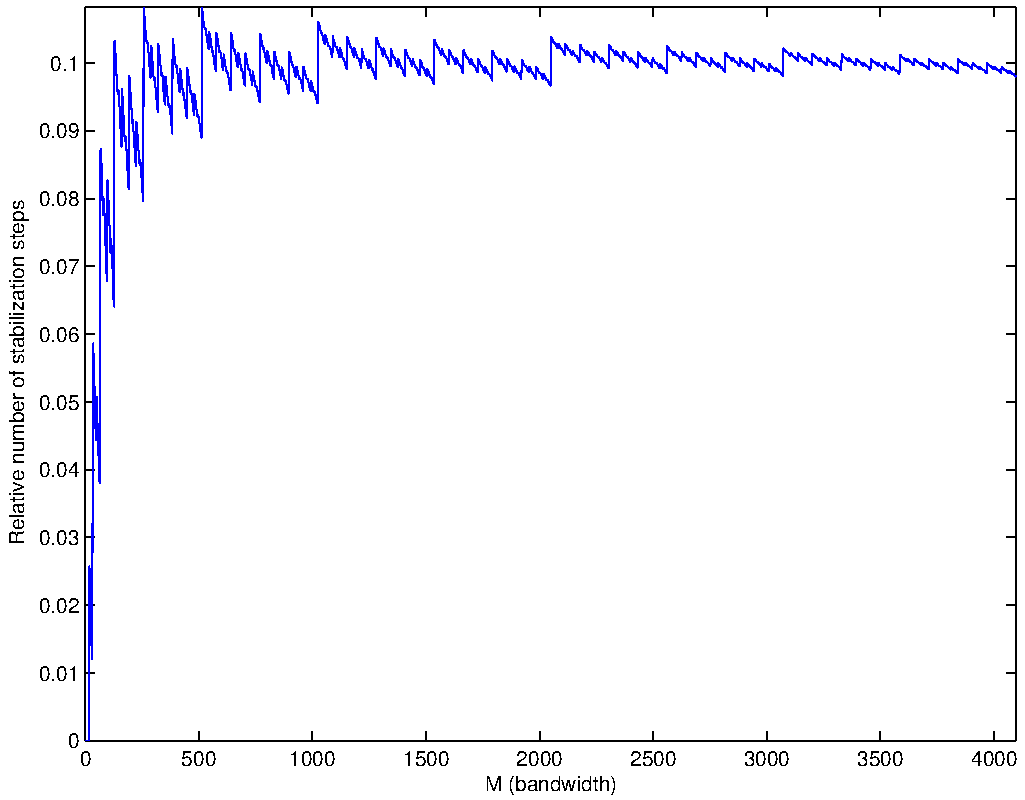
\includegraphics[width=0.5\textwidth]{images/stabilization1000}}\hfill
   \subfigure
     {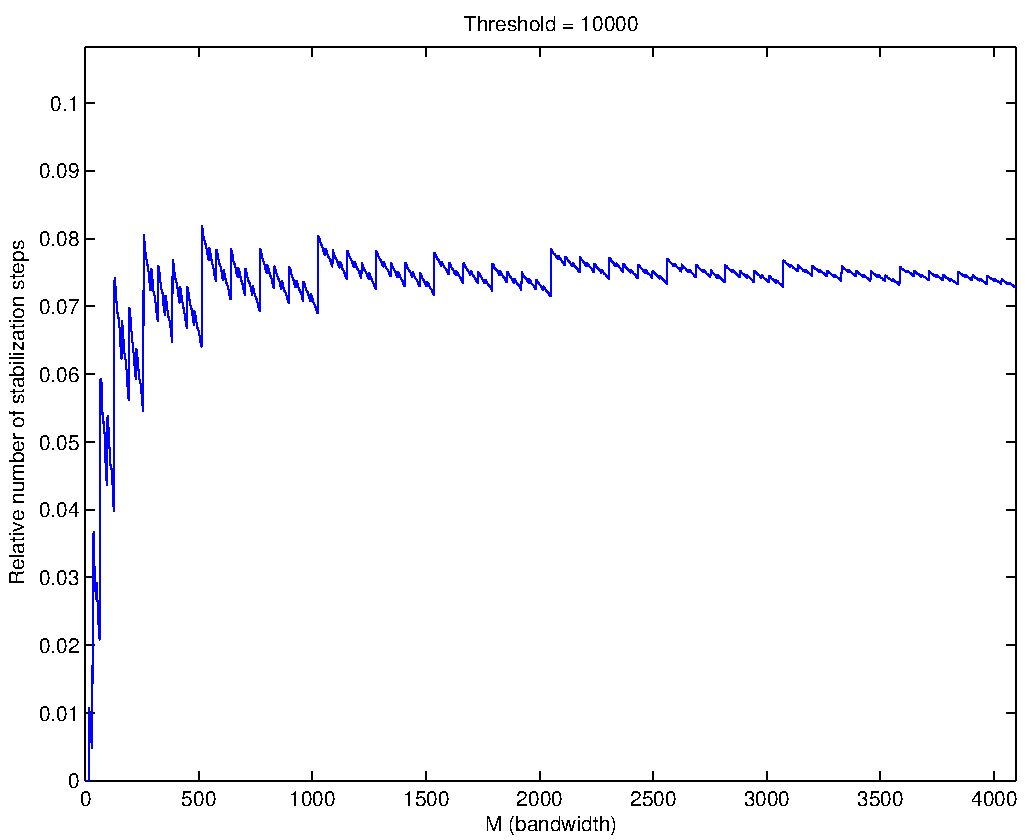
\includegraphics[width=0.5\textwidth]{images/stabilization10000}}\\
   \subfigure
     {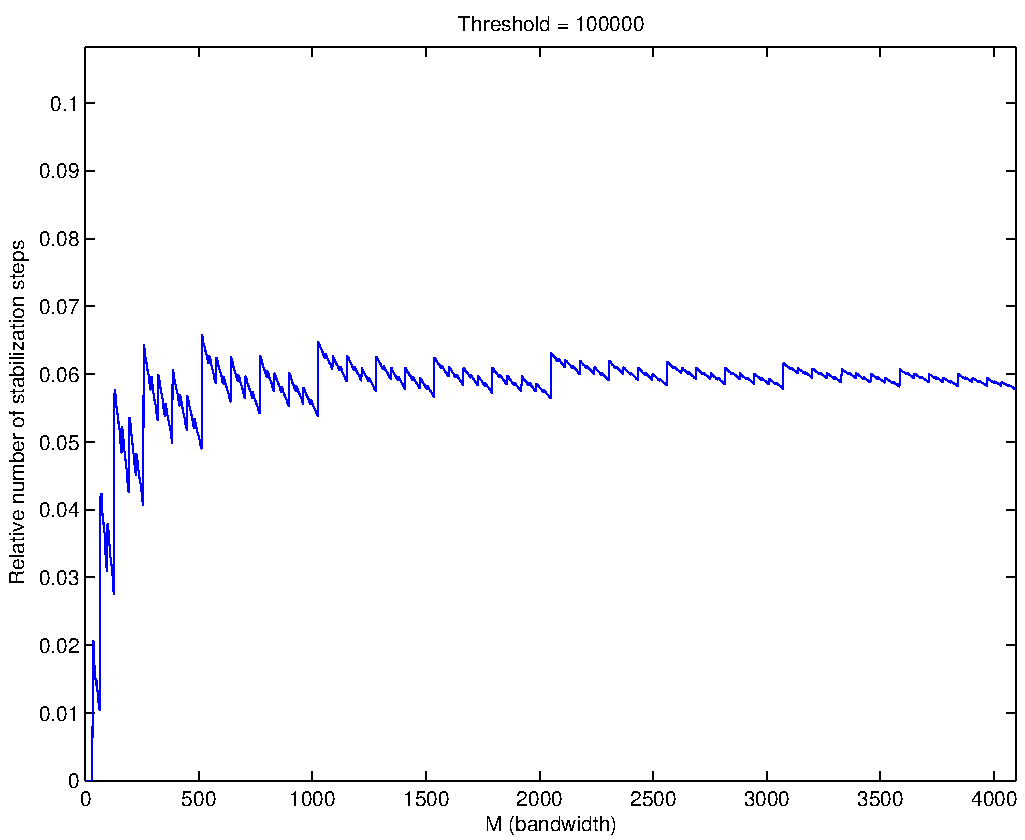
\includegraphics[width=0.5\textwidth]{images/stabilization100000}}\hfill
   \subfigure
     {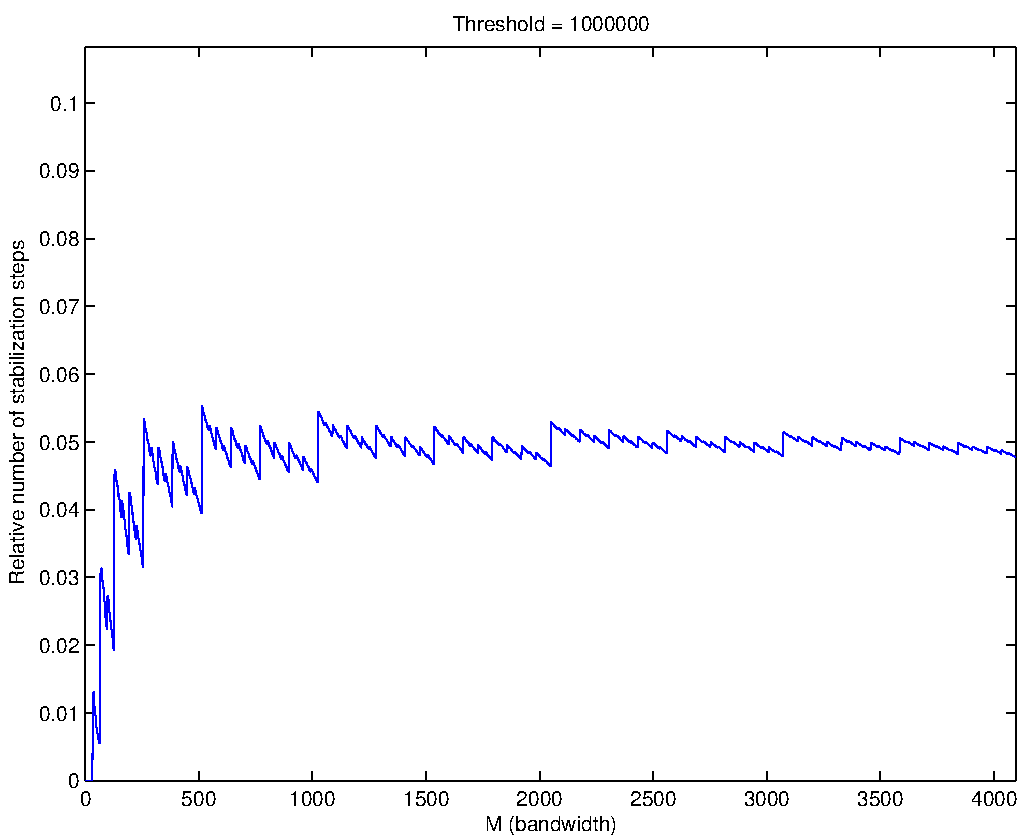
\includegraphics[width=0.5\textwidth]{images/stabilization1000000}}\\
  \caption{The relative number of stabilization steps for thresholds $1000, 10000, 100000$ and $1000000$ and bandwidth $M$ up to $4096$.}
  \label{NFSFT:figure:stabilization}
\end{figure}
Algorithm \ref{NFSFT:Algorithm:FLFT_stab} summarizes the complete algorithm with stabilization.
\begin{algorithm}[htb]
  \caption{Fast Legendre Function transform (stabilized)}
  \label{NFSFT:Algorithm:FLFT_stab}    
  \begin{algorithmic}
    \STATE Input:  $M \in \NZ$, $n \in \NZ$ $(n \le M)$, $\paren{a_k^n}_{k=n}^{M}$
    \STATE Precompute: $t$, $N$, $\tilde{n}$, $\tilde{M}$ as above and $$\fun{U_{2^{\tau}-1}^{n}}{\cos \frac{\paren{2s+1}\pi}{2^{\tau+2}}, 2^{\tau+1}l+1}$$ 
    \STATE \invisible{Precompute:} for $\tau = 1,\ldots,t-1$, $l = \floor{\frac{\tilde{n}}{2^{\tau+1}}},\ldots,\ceil{\frac{\tilde{M}+1}{2^{\tau+1}}}-1$, 
    \STATE \invisible{Precompute:} $s = 0,\ldots,2^{\tau+1}$ and the stabilization steps.
    \STATE $a_{0}^{(t-1),\text{stab}} := a_{1}^{(t-1),\text{stab}} := 0$
    \STATE Compute $\paren{a_{k}^{(0)}}_{k=0}^{N-1}$ 
    \FOR {$\tau=1,\ldots,t$}
      \FOR {$l = \floor{\frac{\tilde{n}}{2^{\tau+1}}},\ldots,\ceil{\frac{\tilde{M}+1}{2^{\tau+1}}}-1$} 
        \IF {multiplication with \fun{U_{2^{\tau}-1}^{\abs{n}}}{\cos \frac{\paren{2s+1}\pi}{2^{\tau+2}}, 2^{\tau+1}l+1} is stable}
          \STATE Compute $a_{2^{\tau+1}l}^{(\tau)}$ and $a_{2^{\tau+1}l+1}^{(\tau)}$ from $$a_{2^{\tau+1}l}^{(\tau-1)},\  
            a_{2^{\tau+1}l+1}^{(\tau-1)},\ a_{2^{\tau+1}l+2^{\tau}}^{(\tau-1)},\ a_{2^{\tau+1}l+2^{\tau}+1}^{(\tau-1)}$$ using 
            \eqref{NFSFT:GeneralStep} and Algorithm \ref{Basics:Algorithm:FastPolynomialMultiplication}
        \ELSE
          \STATE Update $a_{0}^{(t-1),\text{stab}}$ and $a_{1}^{(t-1),\text{stab}}$ from
            $$ 
              a_{2^{\tau+1}l+2^{\tau}}^{(\tau-1)},\ a_{2^{\tau+1}l+2^{\tau}+1}^{(\tau-1)}
            $$ 
            using \eqref{NFSFT:StabilizationStep} and Algorithm \ref{Basics:Algorithm:FastPolynomialMultiplication}
          \STATE Update $a_{2^{\tau+1}l^{(\tau)}} := a_{2^{\tau+1}l^{(\tau-1)}}$, $a_{2^{\tau+1}l+1}^{(\tau)} := a_{2^{\tau+1}l+1}^{(\tau-1)}$
        \ENDIF
      \ENDFOR
    \ENDFOR
    \STATE Compute $a_{0}^{(t-1)} := a_{0}^{(t-1)} + a_{0}^{(t-1),\text{stab}}$, $a_{1}^{(t-1)} := a_{1}^{(t-1)} + a_{1}^{(t-1),\text{stab}}$
    \STATE Output: $\paren{c_{k}}_{k=0}^{2N-1}$
\end{algorithmic}
\end{algorithm}

\section{A Linear Algebra Approach}
\label{DSFT:LinearAlgebra}

In this section we represent the FLFT algorithm as a linear mapping acting on a vector of Fourier coefficients $\V{a}^n$, hence a matrix. 
%Let again $n$ with $\abs{n} \le M$ be fixed. 
The FLFT can be represented as a matrix $\V{T} \in \R^{(N+1) \times (N+1)}$ that multiplied with a vector $\V{a}^n = \left(a_0^n,a_1^n,\dots,a_N^n\right)^T \in \C^{N+1}$ of Fourier coefficients gives a vector $\V{b}^n := \left(b_0^n,b_1^n,\dots,b_{2N-1}^n\right)^{\transp} \in \C^{2N}$ containing the Chebyshev coefficients $b_{k}^n$ of the polynomial $\fun{g^n}{x}$ from \eqref{NFSFT:GnEven} or \eqref{NFSFT:GnOdd}, respectively: 
$$\V{b}^{n} = \V{T} \; \V{a}^n.$$ 
For the sake of simplicity we omit the fact that $a_{k}^n = 0$ for $k < n$ or $k > M$ exploited in Algorithm \ref{NFSFT:Algorithm:FLFT_stab} in order to save some computational steps.

The algorithm implies a factorization of $\V{T}$ into sparse matrices that can be derived directly.
%from the algorithm already presented 
We will use this fact to obtain an algorithm for the transposed problem. In general, the FLFT consists of $t+1$ steps such that $\V{T}$ can be written as 
$$
  \V{T} = \V{T}^{(t)} \: \cdot \:  \V{T}^{(t-1)} \: \cdot \: \dots \: \cdot \: \V{T}^{(1)} \: \cdot \:  \V{T}^{(0)},
$$
with
$$
 \V{T}^{(\tau)} \in \left\{\begin{array}{l@{\quad \text{if} \quad}l} \R^{2N \times (N+1)} & \tau = 0, \\ \R^{2N \times 2N} & 1 \le \tau < t, \\ \R^{(N+1) \times 2N} & \tau = t. \end{array}\right.
$$

\subsection{The First Step}

The first step converts each Fourier coefficent $a_{k}^n$ into a polynomial of degree at most 1 in Chebyshev representation $\V{a}_{k}^{(0)} \in \C^2$. The result 
$$
  \V{a^{(0)}} := 
    \left[\begin{array}{c}
      \V{a}_{0}^{(0)}\\
      \vdots\\
      \V{a}_{N-1}^{(0)}
    \end{array}\right] 
    \in \C^{2N}
$$ 
is a vector of length $2N$, hence 
$$ 
  \V{a}_{k}^{(0)} = \V{e} \: a_{k}^n,\quad \text{with } \V{e} := \left(\begin{array}{l}1\\0\end{array}\right) \quad \paren{k = 0,\ldots,N-3}.
$$
The last polynomial $a_{N}^{(0)}$ is mapped to the preceeding two polynomials by means of the three-term recurrence for associated Legendre Functions, 
i.e. 
$$
  a_{N}^{(0)} = \left(\alpha x + \beta\right)a_{N-1}^{(0)} + \gamma a_{N-2}^{(0)}.
$$
Following this, $\V{T}^{(0)}$ can be written as 
$$
  \V{T}^{(0)} = \encl{[}{\V{I}_{N} \otimes \V{e},\;\V{\tilde{e}}}{]},
$$
with $\V{\tilde{e}} := \left(0,0,\dots,0,\gamma, 0, \beta,\alpha\right)^{\transp} \in \R^{2N}$.

\subsection[Cascade Summation]{Steps $\tau = 1,\ldots,t-1$ (Cascade Summation)}
These steps represent the cascade summation applied to associated Legendre functions. In each round, half of the the functions is eliminated by mapping them to the remaining functions. Therefore, the vector $\V{a}^{(\tau-1)}$ is divided into consecutive blocks of four polynomials
$$
  \V{a}^{(\tau-1)} = 
    \left[\begin{array}{c}
      \V{a}^{(\tau-1)}_{0}\\
      \vdots\\
      \V{a}^{(\tau-1)}_{\frac{N}{2^{\tau+1}}-1}
    \end{array}\right]  \in \C^{2N},
$$
with
\begin{equation}
  \nonumber
  \V{a}^{(\tau-1)}_{l} := 
    \left[\begin{array}{l}
      \V{a}^{(\tau-1)}_{2^{\tau+1}l}\\[1ex]
      \V{a}^{(\tau-1)}_{2^{\tau+1}l+1}\\[1ex]
      \V{a}^{(\tau-1)}_{2^{\tau+1}l+2^{\tau}}\\[1ex]
      \V{a}^{(\tau-1)}_{2^{\tau+1}l+2^{\tau}+1}
    \end{array}\right] \in \C^{2^{\tau+2}} \quad \paren{l=0,\ldots,\frac{N}{2^{\tau+1}}-1},
\end{equation}
where $\V{a}^{(\tau-1)}_{2^{\tau+1}l+j} \in \C^{2^{\tau}}$ for $j = 0,1,2^{\tau},2^{\tau}+1$, representing the polynomial factors in front of each remaining function $P_{k}^n$. Each polynomial is represented by its vector of Chebyshev coefficients of length $2^{\tau}$. In every block, the first and the second polynomial, $a^{(\tau-1)}_{2^{\tau+1}l}$
and $a^{(\tau-1)}_{2^{\tau+1}l+1}$ remain unchanged. The third and the fourth polynomial, $a^{(\tau-1)}_{2^{\tau+1}l+2^{\tau}}$ and $a^{(\tau-1)}_{2^{\tau+1}l+2^{\tau}+1}$, are multiplied with the matrix $\fun{\V{U}_{2^{\tau}-1}^{n}}{\cdot,2^{\tau+1}l+1}$ which transforms them into a representation in terms of the first two functions. Following this, the output contains only half of the polynomials, but due to the multiplication with $\fun{\V{U}_{2^{\tau}-1}^{n}}{\cdot,2^{\tau+1}l+1}$ the degree might double each time so that twice the space is needed to store the Chebyshev coefficients. In total, the result vector still has length $2N$. 
%For each step $1 \le \tau < t$ and for each block $$\mb{\tilde{a}}_{l}^{(\tau-1)} := \left(\mb{a}_{4l}^{(\tau-1)},\mb{a}_{4l+1}^{(\tau-1)},\mb{a}_{4l+2}^{(\tau
%-1)},\mb{a}_{4l+3}^{(\tau-1)}\right)^T \text{, where } 0 \le l < 2^{t-\tau-1},$$ 
We need to keep the first two polynomials, but with their vectors zero-padded to twice the length. Furthermore, we have to add the coefficients due to the multiplication of the third and fourth polynomial with the matrix $\fun{\V{U}_{2^{\tau}-1}^{n}}{\cdot,2^{\tau+1}l+1}$.
Correspondingly, each block $\V{a}_{l}^{(\tau-1)}$ is multiplied by a matrix $\V{V}^{(\tau)}_l := \left[\V{Z^{(\tau)}},\V{U}^{(\tau)}_l\right]$, with
$$\V{Z}^{(\tau)} := \left(\begin{array}{cccc} \V{I}_{2^{\tau}} & 0\\ 0 & 0 \\ 0 & \V{I}_{2^{\tau}} \\ 0 & 0 \end{array}\right) \in \R^{2^{\tau+2} \times 2^{\tau+1}},\ \V{U}^{(\tau)}_l \in \R^{2^{\tau+2} \times 2^{\tau+1}}.$$
%Correspondingly, this can be written as the product 
%$$\mb{ZP}_{\tau} \; \mb{\tilde{a}}_{l}^{\tau-1} \text{, with } \mb{ZP}_{\tau} := \left(\begin{array}{cccc} \mb{I}_{2^{\tau}} & 0 & 0 & 0\\ 0 & 0 & 0 & 0 \\ 0 & \mb{I}_{2^{\tau}} & 0 & 0 \\ 0 & 0 & 0 & 0 \end{array}\right) \in \R^{2^{\tau+2} \times 2^{\tau+2}}.$$ 
%The multiplication with the matrix $\mb{U}$ that acts on the third and fourth polynomial is written as $\mb{U}_{\tau}^l \; \mb{\tilde{a}}_{l}^{\tau-1}$ where the matrix can be factorized as follows:
The matrix $\V{U}^{(\tau)}_l \in \R^{2^{\tau+2} \times 2^{\tau+1}}$ can be factorized as follows:
\begin{equation} 
  \label{NFSFT:LinearAlgebra:Factorization}
  \V{U}^{(\tau)}_l := \V{D}^{(\tau)}_{\text{II}} \; \cdot \; \V{S}^{(\tau)} \; \cdot \; \fun{\V{P}^{(\tau)}}{2^{\tau + 1}l+1} \; \cdot \; \V{D}^{(\tau)}_{\text{III}}
\end{equation}
where we define
\begin{align*}
  \V{D}^{(\tau)}_{\text{II}} & := \V{I}_{2} \otimes \left(\V{D}_{2^{\tau+1}} \V{C}_{2^{\tau+1}}\right) & \in \R^{2^{\tau+2} \times 2^{\tau+2}},\\
  \V{S}^{(\tau)} & := \V{I}_2 \otimes \left[\begin{array}{cc}\V{I}_{2^{\tau+1}},\V{I}_{2^{\tau+1}}\end{array}\right] & \in \R^{2^{\tau+2} \times 2^{\tau+3}},\\
  \fun{\V{P}^{(\tau)}}{c} & := \text{diag}\left(\gamma_{c}^n \fun{\V{P}_{2^{\tau}-2}^n}{c+1},\gamma_{c}^n \fun{\V{P}_{2^{\tau}-1}^n}{c+1},\right.\\
    & \left. \hspace{9ex} \fun{\V{P}_{2^{\tau}-1}^n}{c}, \fun{\V{P}_{2^{\tau}}^n}{c}\right) & \in \R^{2^{\tau+3} \times 2^{\tau+3}},\\
  \V{D}^{(\tau)}_{\text{III}} & := \V{I}_{2} \otimes \left(\left(\V{I}_{2} \otimes \V{C}^{\transp}_{2^{\tau+1}}\right)\V{Z}^{(\tau)}\right) & \in \R^{2^{\tau+3} \times 2^{\tau+1}}.
\end{align*}   
This follows directly from Algorithm \ref{NFSFT:Algorithm:FLFT_unstab}. The matrix $\V{D}^{(\tau)}_{\text{III}}$ realizes first the zero-padding ($\V{Z}^{(\tau)}$)
of the two polynomials $a^{(\tau-1)}_{2^{\tau+1}l+2^{\tau}}$ and $a^{(\tau-1)}_{2^{\tau+1}l+2^{\tau}+1}$, second the evaluation at the Chebyshev nodes ($\V{\tilde{C}}^{\transp}$) and finally a duplication of the result vector in order to permit multiplication with two different associated Legendre polynomials for each polynomial. The matrix $\fun{\V{P}^{(\tau)}}{2^{\tau+1}l+1}$ contains on its main diagonal the associated Legendre polynomials of the matrix $\fun{\V{U}_{2^{\tau}-1}^n}{\cdot,2^{\tau+1}l+1}$ evaluated at the Chebyshev nodes. It realizes therefore a pointwise multiplication with the zero-padded and evaluated polynomials $a^{(\tau-1)}_{2^{\tau+1}l+2^{\tau}}$ and $a^{(\tau-1)}_{2^{\tau+1}l+2^{\tau}+1}$. The matrix $\V{S}^{(\tau)}$ forms the sums for the two rows of the result and finally the $\V{D}^{(\tau)}_{\text{II}}$ transforms the new obtained polynomials $a^{(\tau)}_{2^{\tau+1}l}$ and $a^{(\tau-1)}_{2^{\tau+1}l+1}$ back into Chebyshev representation.

From the factorization in \eqref{NFSFT:LinearAlgebra:Factorization} the more compact representation
\begin{equation}
\label{UCompact}
\V{U}^{(\tau)}_l = 
\left(\begin{array}{lclrcr}
  \V{D}_{2^{\tau+1}} \V{C}_{2^{\tau+1}} & \gamma_{c}^n & \left(\right. & \fun{\V{P}_{2^{\tau}-2}^n}{c+1} \V{C}^{\transp}_{2^{\tau+1}} \V{Z}_{1} & + & 
  \fun{\V{P}_{2^{\tau}-1}^n}{c+1} \V{C}^{\transp}_{2^{\tau+1}} \V{Z}_{2} \left.\right) \\
  \V{D}_{2^{\tau+1}} \V{C}_{2^{\tau+1}} & & \left(\right. & \fun{\V{P}_{2^{\tau}-1}^n}{c} \V{C}^{\transp}_{2^{\tau+1}} \V{Z}_{1} & + & 
  \fun{\V{P}_{2^{\tau}}^n}{c} \V{C}^{\transp}_{2^{\tau+1}} \V{Z}_{2} \left.\right)
\end{array}\right)
\end{equation}
is obtained.
%So for each block $l$, a multiplication with a matrix $\mb{V}_{\tau}^l  \in \R^{2^{\tau+2} \times 2^{\tau+2}}$ is applied where
%$$ \mb{V}_{\tau}^l = \left[\mb{ZP},\mb{U}_{\tau}^l\right].$$ 
The complete step can finally be represented as $$\V{T}^{(\tau)} = \text{diag}\left(\V{V}^{(\tau)}_0,\V{V}^{(\tau)}_1,\dots,\V{V}^{(\tau)}_{2^{t-\tau-1}-1}\right).$$

\subsection{The Last Step}
\label{NFSFT:LinearAlgebra:LastStep}
The last step consists in calculating the polynomial $g^{n} = a_{0}^{(t-1)} P_{0}^{n} + a_{1}^{(t-1)} P_{1}^{n}$ in Chebyshev representation. Since 
$$
  \fun{P_{0}^n}{x} = \frac{\left( \left( 2n \right) ! \right)^{1/2}}{2^n n!},\ \fun{P_{1}^n}{x} = \left(\alpha_{0}^n x + \beta_{0}^n\right)P_{0}^n(x),
$$ 
we can use 
$$
  xT_{0}(x) = T_{1}(x),\ xT_{k}(x) = \frac{1}{2}\left( T_{k+1}(x) + T_{k-1}(x) \right)
$$ 
to write
$$ 
  \V{g}^{n} = \gamma_{0}^n \left( \V{I}_{N+1} \V{a}_{0}^{(\tau-1)} + \left( \alpha_{0}^n\V{W}_{N+1} + \beta_{0}^n\V{I}_{N+1} \right) \V{a}_{1}^{(\tau-1)} \right).
$$
Here, we have defined
$$
\mb{W}_{k} :=
\left(
\begin{array}{ccccccc}
  0 & \frac{1}{2} &             &                           \\
  1 &           0 & \frac{1}{2} &                           \\
    & \frac{1}{2} &           0 & \ddots                    \\
    &             &      \ddots & \ddots      & \frac{1}{2} \\
    &             &             & \frac{1}{2} &           0
\end{array}
\right)
\in \R^{k \times k} \quad \paren{k \in \N}.
$$
Depending on $n \in \NZ$, we can distinguish three cases:
\begin{description}
  \item[n odd] In this case, $\alpha_{0}^n = 0$ and $\beta_{0}^n = 1$ so that $\V{T}^{(\tau)}$ is 
    $$
      \V{T}^{(\tau)} = \gamma_{0}^n \left[ \V{I}_{N+1}, \V{I}_{N+1} \right].
    $$
  \item[n = 0] Here it holds, $\alpha_{0}^n = 1$ and $\beta_{0}^n = 0$ and we get $$\V{T}^{(\tau)} = \gamma_{0}^n \left[ \V{I}_{N+1}, \V{W}_{N+1} \right].$$
  \item[n even, n > 0] Now $\alpha_{0}^n = -1$ and $\beta_{0}^n = 1$ which results in $$\V{T}^{(\tau)} = \gamma_{0}^n \left[ \V{I}_{N+1}, \V{I}_{N+1} - \mb{W}_{N+1} \right].$$
\end{description}

\section{Transposed FLFT}
Following the factorization of $\V{T}$ given in the previous section, one obtains easily the transposed factorization corresponding to $\V{T^{\transp}}$:
$$
  \V{T}^{\transp} = {\V{T}^{(0)}}^{\transp} \: \cdot \: {\V{T}^{(1)}}^{\transp} \: \cdot \: \ldots \: \cdot {\V{T}^{(t-1)}}^{\transp} \: \cdot \: {\V{T}^{(t)}}^{\transp}.
$$ 
For $\tau = 0$ and $\tau = t$ we obtain immediatly
$$
  {\V{T}^{(0)}}^{\transp} = 
     \left(\begin{array}{c} 
       \V{I}_{N} \otimes \V{e}_{1}^{\transp}\\ 
       \V{\tilde{e}}^{\transp} 
     \end{array}\right),\  
   {\V{T}^{(t)}}^{\transp} = \gamma_{0}^n 
     \left\{\begin{array}{l@{\quad \text{if} \quad}l} 
       \left[ \begin{array}{c} \V{I}_{N+1} \\ \V{I}_{N+1}                         \end{array} \right] & \text{$n$ odd},          \\[2ex]
       \left[ \begin{array}{c} \V{I}_{N+1} \\               \V{W}_{N+1}^{\transp} \end{array} \right] & \text{$n = 0$},          \\[2ex]
       \left[ \begin{array}{c} \V{I}_{N+1} \\ \V{I}_{N+1} - \V{W}_{N+1}^{\transp} \end{array} \right] & \text{$n$ even, $n$ > 0}.
     \end{array}\right.
$$
For the rest of the steps, i.e. $\tau = t-1,\ldots,1$, we have
\begin{eqnarray*}
 {\V{T}^{(\tau)}}^{\transp}   & = & \text{diag}\left({\V{V}^{(\tau)}_0}^{\transp},{\V{V}^{(\tau)}_1}^{\transp},\dots,{\V{V}^{(\tau)}_{2^{t-\tau-1}-1}}^{\transp}\right),\\
 {\V{V}^{(\tau)}_l}^{\transp} & = & \left[ \begin{array}{c} \V{Z}^{\transp},\\ 
 {\V{U}^{(\tau)}_l}^{\transp} \end{array} \right],\\
 {\V{U}^{(\tau)}_l}^{\transp} & = &
   \left(\begin{array}{rlllr}
     \gamma_{c}^n & \left(\right. \V{Z}_{1}^{\transp} \V{\tilde{C}}_{2^{\tau+1}} \fun{\V{P}_{2^{\tau}-2}^n}{c+1} & + & \V{Z}_{2}^T \V{\tilde{C}}_{2^{\tau+1}} \fun{\V{P}_{2^{\tau}-1}^n}{c+1}                  & \left.\right) \V{\tilde{C}}_{2^{\tau+1}}^{\transp} \\
                  & \left(\right. \V{Z}_{1}^{\transp} \V{\tilde{C}}_{2^{\tau+1}} \fun{\V{P}_{2^{\tau}-1}^n}{c} & + & \V{Z}_{2}^{\transp} \V{\tilde{C}}_{2^{\tau+1}} \fun{\V{P}_{2^{\tau}}^n}{c} & \left.\right) \V{\tilde{C}}_{2^{\tau+1}}^{\transp}
     \end{array}
   \right).
\end{eqnarray*}

%
%\begin{figure}[tb]
%  \centering
%  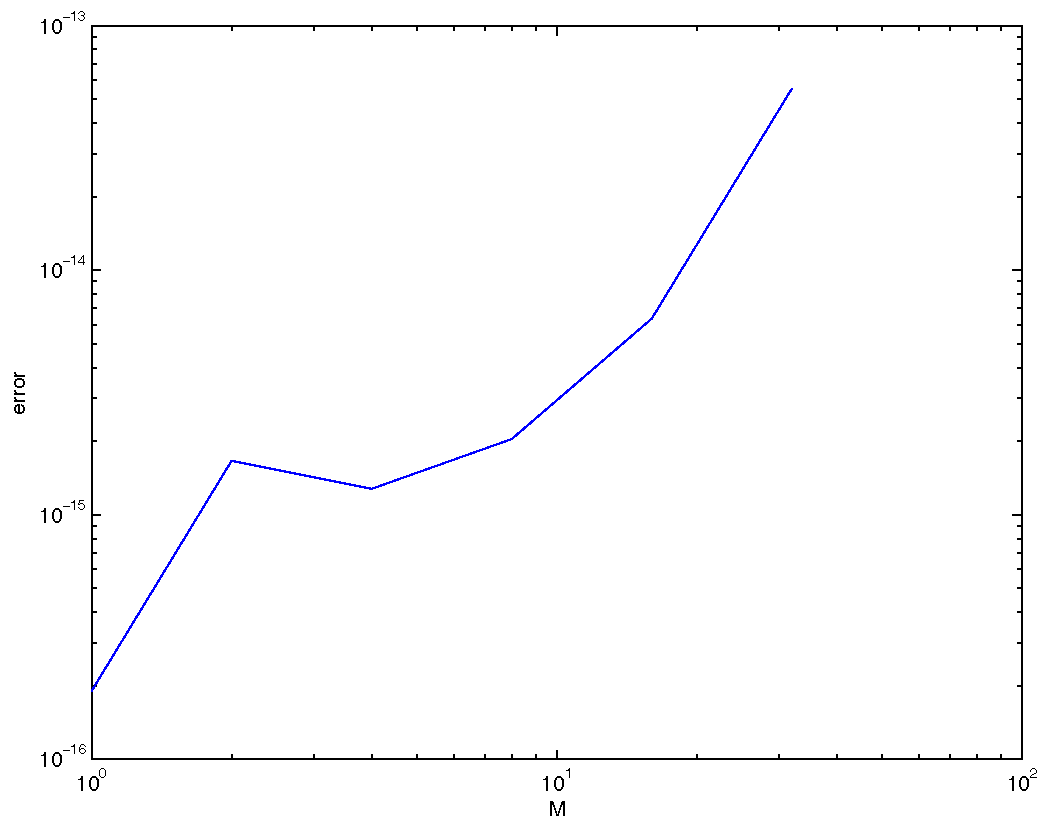
\includegraphics[height=9cm,width=12cm]{images/accuracy}
%  \caption{To be written...}
%  \label{NFSFT:Figure:Accuracy}
%\end{figure}


\section{Adjoint Fast Spherical Fourier Transform}
\label{DSFT:AdjointTransform}
\chapter{The Inverse Problem}
\label{iDSFT}

\section{}

\chapter{Numerical Results}
\label{NumericalResults}
\bibliographystyle{abbrv}
\bibliography{ref}



\backmatter

\end{document}  